\documentclass{book}


\usepackage{lipsum}
\usepackage{amsmath, amsthm, amssymb, amsfonts,mathrsfs}
\usepackage{thmtools}
\usepackage{graphicx}
\usepackage{setspace}
\usepackage{enumitem}
\usepackage{zhlipsum}
\usepackage{geometry}
\geometry{
  a4paper,
  top=25.4mm, bottom=25.4mm,
  left=20mm, right=20mm,
  headheight=2.17cm,
  headsep=4mm,
  footskip=12mm
}
\usepackage{float}
\usepackage{hyperref}
\usepackage[utf8]{inputenc}
\usepackage[english]{babel}
\usepackage{framed}
\usepackage[dvipsnames]{xcolor}
\usepackage{tikz-cd}
\usepackage[most]{tcolorbox}
\usepackage{ctex}
\usepackage{colortbl}
\usepackage{pifont}
\usepackage{framed}
\definecolor{shadecolor}{RGB}{241, 241, 255}
\newcounter{problemname}

\tcbuselibrary{theorems}
\tcbuselibrary{breakable}
\hypersetup{hidelinks,
	colorlinks=true,
	allcolors=black,
	pdfstartview=Fit,
	breaklinks=true
}

%定义颜色,可以根据需求自己修改
\definecolor{LightIndigo}{HTML}{E0FFFF}
\colorlet{LightGray}{White!90!Periwinkle}
\colorlet{LightOrange}{Orange!15}
\colorlet{LightGreen}{Green!15}
\colorlet{Lightblue}{Blue!15}
\colorlet{Lightpurple}{Purple!15}
\colorlet{LightRed}{Red!15}
\colorlet{LightYellow}{Yellow!15}
\colorlet{LightCyan}{Cyan!15}
%\colorlet{LightIndigo}{E0FFFF}

\newcommand{\HRule}[1]{\rule{\linewidth}{#1}}

\newtheorem{corollary}{Corollary}[section]
\newenvironment{solution}{{\noindent\it Solution.} }{\hfill $\square$\par}
\newenvironment{note}{\noindent\it Note.}{\par}

\declaretheoremstyle[name=Theorem,]{thmsty}
\declaretheorem[style=thmsty,numberwithin=chapter]{theorem}
\tcolorboxenvironment{theorem}{colback=LightGray,breakable,before upper app={\setlength{\parindent}{2em}}}

\declaretheoremstyle[name=Definition,]{thmsty}
\declaretheorem[style=thmsty,numberwithin=chapter]{definition}
\tcolorboxenvironment{definition}{colback=LightCyan,breakable,before upper app={\setlength{\parindent}{2em}}}

\declaretheoremstyle[name=Remark,]{thmsty}
\declaretheorem[style=thmsty,numberwithin=chapter]{remark}
\tcolorboxenvironment{remark}{colback=LightRed,breakable,before upper app={\setlength{\parindent}{2em}}}

\declaretheoremstyle[name=Lemma,]{thmsty}
\declaretheorem[style=thmsty,numberwithin=chapter]{lemma}
\tcolorboxenvironment{lemma}{colback=Lightblue,breakable,before upper app={\setlength{\parindent}{2em}}}

\declaretheoremstyle[name=Corollary,]{thmsty}
\declaretheorem[style=thmsty,numberwithin=chapter]{Corollary}
\tcolorboxenvironment{corollary}{colback=Lightpurple,breakable,before upper app={\setlength{\parindent}{2em}}}

\declaretheoremstyle[name=Proposition,]{prosty}
\declaretheorem[style=prosty,numberwithin=chapter]{proposition}
\tcolorboxenvironment{proposition}{colback=LightOrange,breakable,before upper app={\setlength{\parindent}{2em}}}

\declaretheoremstyle[name=Example,]{prosty}
\declaretheorem[style=prosty,numberwithin=chapter]{example}
\tcolorboxenvironment{example}{colback=LightGreen,breakable,before upper app={\setlength{\parindent}{2em}}}

\declaretheoremstyle[name=Exercise,]{prosty}
\declaretheorem[style=prosty,numberwithin=chapter]{exercise}
\tcolorboxenvironment{exercise}{colback=LightYellow,breakable,before upper app={\setlength{\parindent}{2em}}}

\setstretch{1.2}
\geometry{
    textheight=9in,
    textwidth=5.5in,
    top=1in,
    headheight=12pt,
    headsep=25pt,
    footskip=30pt
}
\usepackage{ulem}
\usepackage{pdfpages}
\usepackage{soul}
\usepackage{etoolbox}
\usepackage{graphicx}
\usepackage{multicol}
\usepackage{multirow}
\usepackage{amsmath}
\usepackage{amssymb}
\usepackage{hyperref}
\usepackage{cleveref}
\usepackage{annotate-equations}
\usepackage{enumitem}
\usepackage{zhlipsum}
\usepackage{enumitem}
\usepackage{zhlipsum}
\usepackage{enumitem}
\usepackage{amsmath}
\usepackage{amssymb}
\usepackage{hyperref}
\usepackage{accents}
\usepackage{cleveref}
\usepackage{annotate-equations}
\usepackage{bbm}
\usepackage{diagbox}
\usepackage{enumerate}
\definecolor{SwishLineColour}{HTML}{88AC0B}
\definecolor{MarkerColour}{HTML}{B6073F}
\usetikzlibrary{positioning}
%\newenvironment{procedure}
%{\begin{shaded}\par\noindent\textbf{procedure}\quad\par\noindent}{\end{shaded}\par}

\declaretheoremstyle[name=Procedure,]{prosty}
\declaretheorem[style=prosty,numberwithin=section]{procedure}
\tcolorboxenvironment{procedure}{colback=LightIndigo,breakable,before upper app={\setlength{\parindent}{2em}}}


\newcommand*\circled[1]{\tikz[baseline=(char.base)]{
            \node[shape=circle,draw,inner sep=2pt] (char) {#1};}}

\linespread{1.5}
\title{ \normalsize \textsc{Notes of Operation Research}
		\\ [2.0cm]
		\HRule{1.5pt} \\
		\LARGE \textbf{\uppercase{运筹学笔记}
		\HRule{2.0pt} \\ [0.6cm] \LARGE{Jinhua Wu} \vspace*{10\baselineskip}}
		}
\date{}
\author{}

\begin{document}
\maketitle
\tableofcontents 
\newpage
\setcounter{page}{1}
\chapter{Optimisation Theory}
\begin{center}
    \textbf{Assessment:} 70\% examination, 30\% homework
    
    Six assignments:

7\% the first three assignments and 3\% the last three assignments.
\end{center}
\section{Linear Programming}
LP in standard form: 
\begin{align}
    \max {} f & = \sum\limits_{j=1}^n c_j x_j \nonumber \\
    \sum\limits_{j=1}^n a_{ij}x_j & = b_i \text{, } 1\le i\le m \nonumber \\
    x_j & \ge 0 \text{, } 1\le j\le n \label{LP standard}
\end{align}

In matrix form: 
\begin{align}
    \max {} f &= C^T x \nonumber \\
    Ax &= b\nonumber \\
    x & \ge 0 \label{LP matrix}
\end{align}
where $A\in\mathbb{R}^{m\times n}$, $b\in\mathbb{R}^m$, $c\in\mathbb{R}^n$ are given, $x\in\mathbb{R}^n$ is the \textcolor{red}{\textbf{optimisation variable}}. $m<n$, $A$ has the full rank. That is $rank(A) = m$.

\begin{itemize}
    \item $f = C^T x$ is the objective function.
    \item $R = \left\lbrace x\in\mathbb{R}^n, Ax = b, x\ge 0 \right\rbrace$ is the feasible set. If $x\in R$, then $x$ is feasible. Thus $R$ is the intersection of a \textcolor{red}{plane} $Ax = b$ with the \textbf{positive quadrant} $x\ge 0$.
\end{itemize}

\subsection{Simplex Method}

Aim: we want an effective method to solve the LP problem.

Def: The LP(1.1) is non-degenerate if $b$ is not a linear combination of $<m$ columns of $A$. In other words, we can't have $Ax = b$ with $x$ having $<m$ non-zeros entries.

\textit{All our problems will be non-degenerate.}

\bigskip \noindent \textbf{Def} Give the LP(1.1), a basic solution $x\in\mathbb{R}^n$ is as follows. Let $B\in\mathbb{R}^{m\times m}$ be a sub-matrix of $A$ with full rank $m$. Suppose $B$ occupies columns $j_1<j_2<\cdots<j_m$. Let $y = B^{-1}b$. Then 
$$
    x_j = \left\lbrace 
    \begin{array}{ll}
        0 & \text{if } j\notin \left\lbrace j_1, j_2, \cdots, j_m \right\rbrace \\
        y_l & \text{if } j = j_l 
    \end{array}
    \right.
$$

Note that $Ax = by =b$. If also $x\ge 0$, then $x\in\mathbb{R}$, and $x$ is a basic feasible solution.\\

\subsection{Definition}
\begin{itemize}
    \item $S\subset \mathbf{R}^n$ is convex if $\forall x, y\in S$ is an extreme point if $\exists x,y\in S$, $x\neq y$ and $\lambda\in(0, 1)$, s.t. $z = (1-\lambda)x + \lambda y\in S$. Note that $S = \varnothing$ and $S = \left\lbrace x\right\rbrace$ are convex.
    \item If $S\subset \mathbb{R}^n$ is convex, then $z\in S$ is an extreme point if $ \nexists x,y\in S$, $x\neq y$ and $\lambda\in(0,1)$, s.t. $z = (1 -\lambda)x + \lambda y$.
\end{itemize}

\begin{figure}
    \centering
    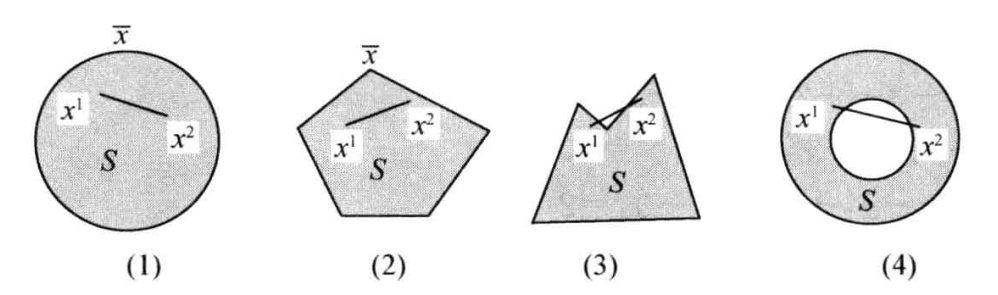
\includegraphics[scale=0.2]{picture_1.png}
    \caption{In this figure, the panel (1)-(2) are convex. Panel (3)-(4) are not convex.}
    \label{fig:enter-label}
\end{figure}

\subsection{Prop 1.1  }
\begin{proposition}
    In the LP (\ref{LP standard}), R is convex.
\end{proposition}

\textit{Proof: } Let $x, y\in R$ and $\lambda\in [0, 1]$. Then 
\begin{equation}
    A\left((1-\lambda)x + \lambda y\right) = (1-\lambda)Ax + \lambda Ay = b\nonumber
\end{equation}
and
\begin{equation*}
    (1-\lambda)x + \lambda y \ge 0
\end{equation*}
since $x, y \ge 0$ and $1-\lambda, \lambda\ge 0$. Thus, $(1-\lambda)x + \lambda y\in R$.

By Prop 1.1, $R$ is convex. Thus in 1.2, 1.3 below, we do have the notion of an extreme point of $R$.

\subsection{Th 1.2}\label{Th 1.2}
\begin{theorem}
    Suppose the LP (\ref{LP standard}) has an optimal solution. Then $R$ has an extreme point which is an optimal solution.
\end{theorem}

\begin{proof}
    Suppose $x^*\in R$ is optimal, but not extreme. Then we have $x^* = (1-\lambda)y + \lambda z$, for some $y, z\in R$, $y\neq z$ and $\lambda \in (0, 1)$. Now $c^Tx^* = (1-\lambda)c^Ty + \lambda c^T z\le (1-\lambda)c^Tx^* + \lambda c^T x^* = c^T x^*$. So $c^Tx^* = c^Ty = c^Tz$. Thus, $c^T\left( (1-\lambda')y+\lambda'z \right) = c^Tx^*$, $\forall \lambda'\in R$. That is, all feasible points on the line through $x^*, y, z$ are optimal.

Let $u = z-y$. Then $A(x^*+\mu u) = Ax^* + \mu Az - \mu Ay = b$. Since $u\neq 0$, assume $J = \left\lbrace 1\le j\le n: u_j <0 \right\rbrace$ satisfy $J\neq\varnothing$. (Otherwise consider $u = y-z$.) Then, we may choose $\mu'>0$ maximum such that $x^*+\mu'u \ge 0$, that $(x^* + \mu' u)_j = 0$ for some $j\in J$. Now, for $1\le j\le n$, $x^*_i = 0\Longrightarrow y_i = z_i = 0$. (since $x^*_i = (1-\lambda)y_i + \lambda z_i$ and $y_iz_i\ge 0$) That means that $\Longrightarrow u_i = 0\Longrightarrow (x^* +\mu'u)_i = 0$. Thus $i\notin J$ for such $i$. We see that $x^* + \mu' u\in R$ has more zero coordinates than $x^*$, and $x^* + \mu' u$ is also optimal.

Repeat this argument, we must stop since we can't have more that $n$ zeros. Upon termination, we have an extreme point of $R$, which is optimal.
\end{proof}

\subsection{Th 1.3}\label{Th 1.3}
\begin{theorem}
    Suppose the LP (\ref{LP standard}) is non-degenerate. Let $x\in R$, then $x$ is extreme $\Longleftrightarrow$ $x$ is a basic feasible solution.
\end{theorem}
\begin{proof}
    $\Longrightarrow$ Suppose $x\in R$ is extreme, but not a basic feasible solution. Let $J = \left\lbrace 1\le j\le n:x_j>0 \right\rbrace$. Suppose first that $|J|\le m$. Then either $|J|< m $ or $|J| = m$. And the columns of $A$ indexed by $J$ are linearly dependent. In either case, $b$ is a linear combination of less than $m$ columns of $A$, which contradicts non-degeneratecy.

    Now, let $|J|>m$. Them the columns of $A$ indexed by $J$ are linearly dependent. If $A'$ is the submatrix of $A$ with these columns, then $\exists v'\in \mathbb{R}^{|J|}\backslash \left\lbrace 0 \right\rbrace$ such that $A'v' = 0$. Extend $v'$ to $v\in \mathbb{R}\backslash\left\lbrace 0 \right\rbrace$ by adding zeros to the remaining coordinators (not indexed by $J$). Then $Av = 0$, and $x_i =0 \Longrightarrow v_i = 0$. Now, $x\pm \varepsilon v\in R$ if $\varepsilon > 0$ is small: $A(x\pm \varepsilon v) = Ax = b$, and $x\pm\varepsilon v\ge 0$ for $\varepsilon>0$ small (since $x_i = 0 \Longrightarrow v_i = 0$). Thus $x = \frac{1}{2}(x+\varepsilon v) + \frac{1}{2} (x - \varepsilon v)$, contradicting $x$ extreme.
\end{proof}

\medskip $\Longleftarrow$ Suppose $x\in R$ is a basic feasible solution, but not extreme. Then $x = (1-\lambda)y+\lambda z$ for some $y, z\in R$, $y\neq z$ and $\lambda\in(0, 1)$. Let $B\in \mathbb{R}^{m\times m}$ bet the submatrix of $A$ corresponding to $x$, and $J\subset\left\lbrace 1, 2, \cdots, n\right\rbrace$ be the index set of the columns of $B$. We have $|J| = m$ and $\text{rank}(B) = m$. For $i\notin J$, we have $x_i = 0\Rightarrow y_i = z_i = 0$(as in \textbf{Th 1.2}). Let $y', z'\in \mathbb{R}^m$ be obtained from $y, z$ by deleting the zeros corresponding to $\left\lbrace 1, 2, \cdots, n\right\rbrace\backslash J$. Then $b = Ay = By'$, $b = Az = Bz'\Rightarrow$$B(y'-z')=0$. But $y'-z'\neq 0$, so $\text{rank}(B) < m$, contradiction.

\subsection{Cor 1.4}\label{Cor 1.4}
\noindent Now \textbf{\ref{Th 1.2} and \ref{Th 1.3}}$\Longrightarrow$ 
\begin{corollary}
    Suppose the LP(\ref{LP standard}) has an optimal solution and is non-degenerate. Then $\exists$ basic feasible solution which is optimal.
\end{corollary}

\subsection{Simplex Method(单纯形法)}\label{Simplex Method}
Now we present the \textbf{simplex method} for solving the LP(\ref{LP standard}). By \textbf{\ref{Cor 1.4}}, to find the maximum of $f$, it suffices to check the value of f at basic feasible solutions. There are $\le \tbinom{n}{m}$ such points, since there are $\le \tbinom{n}{m}$ choices for the submatrix $B$ of $A$. But the idea is, we move from one basic feasible solution to another, and strictly increase $f$ each time. When this procedure stops, we either have an optimal solution, or conclude that there are none.

In (\ref{LP standard}), we treat $f$ as another variable. We have the system:

\begin{equation}
    \left\lbrace\begin{array}{r}
       Ax =b  \\
       -c^Tx + f=0\\
       x \ge0
    \end{array}   \right.\nonumber
\end{equation}

The system is the initial system of the LP \ref{LP standard}. We describe the simplex method, using Example 1.

\noindent \textbf{Example 1} Again consider Example 1. which has the standard from \ref{LP matrix}. The initial system is:
\begin{equation}
    \left\lbrace\begin{array}{ccccccc}
     x_1 &+x_2 & +s_1 &&&   &=6  \\
     2x_1 &+4x_2 &&+s_2&&& = 16\\
     &x_2&&&+s_3&&=3\\
     -3x_1&-4x_2&&&&+f&=0\\
       x_1,&x_2,&s_1,&s_2,&s_3&  &\ge 0
    \end{array}    \right.\nonumber
\end{equation}

We form the simplex table as follows:
\begin{center}
    \begin{tabular}{cccccc|c}
        $x_1$ & $x_2$ & $s_1$ & $s_2$ & $s_3$ & $f$ & \\
        \hline
        1 & 1 & 1 & 0 & 0 & 0 & 6\\
        2 & 4 & 0 & 1 & 0 & 0 & 16\\
        0 & 1 & 0 & 0 & 1 & 0 & 3\\
        \hline
        -3 & -4 & 0 & 0 & 0 & 1 & 0\\
        \hline
    \end{tabular}
\end{center}

Note that $(x_1, x_2, s_1, s_2, s_3) = (0, 0, 6, 16, 3)$ is a basic feasible solution,  and $f = 0$. We require that the entries on the right are $\ge =$. We choose an entry called the \textcolor{red}{\textbf{pivot}} as follows.

\ding{192} Choose the column containing the most negative entry in the bottom row, containing $-4$. We choose this since the objective function is $f = 3x_1 + 4x_2$, so increasing along $x_2$ is the most beneficial.

\ding{193} Next, for each positive entry in the chosen column, (expect for the bottom one), divide the number on the right by the entry. Choose the row with the minimum answer, which is the third row, with $3/1 = 3$. We choose this row so that all three equality constraints of \ref{LP matrix} can be satisfied when $x_2\le 3$. 

The \textbf{pivot} is the entry in the chosen column and row.

\ding{194} We now reduce by making the pivot 1(here, it already is) and all other entries in the second column 0. We do not switch rows.

\begin{center}
    \begin{tabular}{cccccc|c}
    $x_1$ & $x_2$ & $s_1$ & $s_2$ & $s_3$ & $f$ & \\
    \hline
    1 & 0 & 1 & 0 & -1 & 0 & 3\\
    2(pivot) & 0 & 0 & 1 & -4 & 0 & 4\\
    0 & 1 & 0 & 0 & 1 & 0 & 3\\
    \hline
    \textcolor{red}{-3} & 0 & 0 & 0 & -4 & 1 & 12\\
    \hline
\end{tabular}
\end{center}

We have now moved to the basic feasible solution $(x_1, x_2, s_1, s_2, s_3) = (0, 3, 3, 4, 0)$ and $f = 12$. The value of $f$ has increased.

If we still have negative entry in the entry in the bottom row, repeated the procedure. Continue until this ends.

\begin{center}
    \begin{tabular}{cccccc|c}
    $x_1$ & $x_2$ & $s_1$ & $s_2$ & $s_3$ & $f$ & \\
    \hline
    0 & 0 & 1 & -1/2 & 1 & 0 & 1\\
    1 & 0 & 0 & 1/2 & -2(pivot) & 0 & 2\\
    0 & 1 & 0 & 0 & 1 & 0 & 3\\
    \hline
    0 & 0 & 0 & 3/2 & \textcolor{red}{-2} & 1 & 18\\
    \hline
\end{tabular}
\end{center}

\begin{center}
    \begin{tabular}{cccccc|c}
    $x_1$ & $x_2$ & $s_1$ & $s_2$ & $s_3$ & $f$ & \\
    \hline
    0 & 0 & 1 & -1/2 & 1 & 0 & 1\\
    1 & 0 & 2 & 1/2 & 0 & 0 & 4\\
    0 & 1 & -1 & 0 & 0 & 0 & 2\\
    \hline
    0 & 0 & 0 & 2 & 1/2 & 1 & 20\\
    \hline
\end{tabular}
\end{center}

We end at this table since there are no more negative entries in the bottom row, which gives:
\begin{equation}
    f = 20-2s_2-\frac{1}{2}s_3\le 20
\end{equation}
We can read off the final, optimal solution as $(x_1, x_2, s_1, s_2, s_3) = (4, 2, 0, 0, 1)$ and $f=20$. This agrees with the answer in Example 1.

What happens if a LP has no optimal solution?

\begin{example}
    \begin{align*}
        \min&\quad f = -5x_1 + x_2 \\
        & \quad x_1 - x_2 \le 2\\
        & \quad -3x_1 + x_2 \le 0\\
        & \quad x_1, x_2 \ge 0
    \end{align*}
\end{example}
\begin{solution}
    We change the objective function to maximize $f^{\prime}=5x_1 - x_2$.

    Initial system: 
    \begin{equation*}
        \left\lbrace \begin{array}{ll}
          x_1 - x_2 + s_1   &= 2  \\
           -3x_1 +x_2 + s_2  &= 0 \\
           -5x_1 + x_2 + f' & =0 \\
           x_1, x_2, s_1, s_2 &\ge 0
        \end{array}\right.
    \end{equation*}

    Simplex table:

    \begin{center}
    \begin{tabular}{ccccc|c}
    $x_1$ & $x_2$ & $s_1$ & $s_2$ & $f$ & \\
    \hline
    1(pivot) & -1 & 1 & 0 & 0 & 2\\
    -3 & 1 & 0 & 1 & 0 & 0\\
    \hline
    \textcolor{red}{-5} & 1 & 0 & 0 & 1 & 0\\
    \hline
    \end{tabular}
    \end{center}

    \begin{center}
    \begin{tabular}{ccccc|c}
    $x_1$ & $x_2$ & $s_1$ & $s_2$ & $f$ & \\
    \hline
    1 & -1 & 1 & 0 & 0 & 2\\
    0 & -2 & 3 & 1 & 0 & 6\\
    \hline
    0 & -4 & 5 & 0 & 1 & 10\\
    \hline
    \end{tabular}
    \end{center}

    Since no entry in the second column is positive, the LP does not have a solution: there is no finite maximum for $f'$, hence no finite minimum for $f'$. To see this, set $s_1 = 0$, since $s_1$ is a non-basic variable. Set $x_2 = M\ge 0$. Then $(x_1, x_2, s_1, s_2) = (2+M, M, 0, 6+2M)$ is feasible, and $f' = 10+4M\to\infty$ as $M\to\infty$.

    Picture of LP problem:
    \begin{figure}[H]
        \centering
        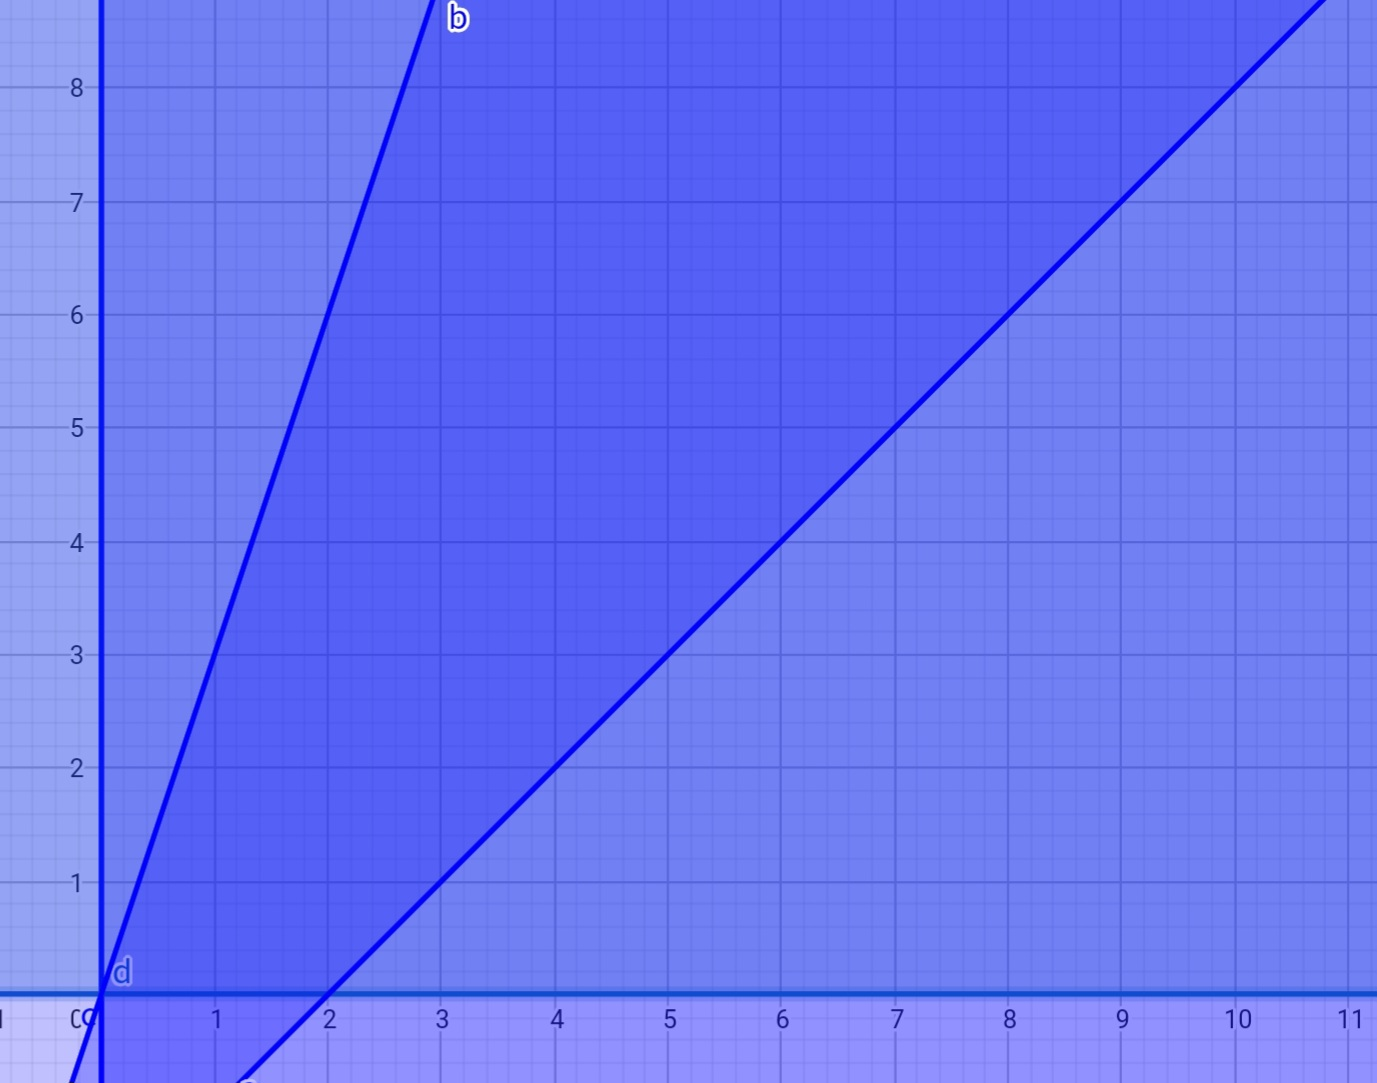
\includegraphics[scale = 0.3]{Screenshot_20240305_083205_Chrome.jpg}
        \label{LP wrong}
    \end{figure}
\end{solution}

\subsection{Procedure of simplex method}
\begin{procedure}
    Give a LP:

    (1) Convert the LP to standard form, introducing slack variables and changing min to max, if necessary. Write down the initial system.

    (2) Write down the simplex table. The entries on the right are $\ge 0$, and some columns form on identity matrix, which gives a basic feasible solution.

    (3) If there is a negative number in the bottom row, choose the column with the most negative number. If there is a tie, choose any such column. If there is no negative number, the optimal solution of the LP is found. Read off the values of the optimal solution and the optimal value.

    (4) For every positive entry in the chosen column from Step 3(except the bottom one), divide the number on the right by the entry. Choose the row with the minimum answer. If there is a tie, choose any such row. If there is no positive entry in the column, then the LP has no optimal solution.

    (5) The entry in the column and row from Step 3 and 4 is the pivot. Perform row operations to make the pivot 1, and other entries in the column 0. Do not exchange rows.

    (6) Repeat Step 3 for the new simplex table. Continue until termination.
\end{procedure}
\begin{remark}
    We note that the simplex method does indeed terminate. There are finitely many basic feasible solutions, $\le \tbinom{n}{m}$. Enough to show that no basic feasible solution is visited more than once. For this, enough to show that $f$ strictly increases in every move. At an iterate, the current value of $f$, say $P$, is in the bottom right of the simplex table. If the pivot is in row $i$ and $P_i\ge 0$ is the entry in the right of row $i$, then the next value for f is $P^{\prime} = P + kP_i$ for some $k>0$. If $P_i = 0$, then we have a basic feasible solution with $<m$ non-zero entries, which contracts non-degeneracy. Hence, $P_i>0$ and $P^{\prime} = P + kP_i > P$.
\end{remark}

\subsection{Duality(对偶)in linear programming}
For $x, y\in\mathbb{R}^n$, write $x\ge y$ to mean $x-y\ge 0$. We write $x\ge y$ to mean $y\ge x$.
\begin{remark}
    Give a LP, we want to associate it with another LP, called the dual.
\end{remark}

Consider the LP: 
\begin{align}
    \max &\quad c^T\boldsymbol{x} \nonumber\\
    &\quad A\boldsymbol{x} \le b \nonumber\\
    &\quad \boldsymbol{x}\ge 0 \label{LP-3}
\end{align}
where $A\in\mathbb{R}^{m\times n}$, $b\in\mathbb{R}^m$, $c\in\mathbb{R}^n$ are given, and $\boldsymbol{x}\in\mathbb{R}^n$ is variable. Let $p^*\in\mathbb{R}$ be the optimal value
\begin{remark}
    $p^* = -\infty$ if (\ref{LP-3}) is not feasible, otherwise $p^*$ is finite or $p^* = +\infty$.
\end{remark} 
We introduce a variable $\boldsymbol{y}\in\mathbb{R}^m$, $\boldsymbol{y}\ge 0$. Then, $\forall \boldsymbol{x}\in \mathbb{R}^n$ feasible for (\ref{LP-3}).
\begin{align}
    \boldsymbol{y}^T A\boldsymbol{x}\le \boldsymbol{y}^T b\quad\text{or}\quad \left(A^T\boldsymbol{y}\right)^T\boldsymbol{x}\le b^T\boldsymbol{y}
\end{align}
If $\boldsymbol{y}$ also satisfies $A^T\boldsymbol{y}\ge c$, then
\begin{equation}
    c^T\boldsymbol{x}\le \left(A^T\boldsymbol{y}\right)^T\boldsymbol{x}\le b^T\boldsymbol{y}\label{y-best}
\end{equation}
Thus, we want to find $\boldsymbol{y}$ such that (\ref{y-best}) is best possible. We define the \textcolor{red}{\textbf{dual}} LP of the LP (\ref{LP-3}) to be:
\begin{align}
    \min &\quad b^T\boldsymbol{y}\nonumber \\
    & \left\lbrace\begin{array}{rl}
        A^T\boldsymbol{y}&\ge c  \\
         \boldsymbol{y}&\ge 0 
    \end{array} \right.\label{dual LP}
\end{align}
where $\boldsymbol{y}\in\mathbb{R}^n$ is a variable. Let $d^*$ be the optimal value.
\begin{remark}
    $d^* = \infty$ if (\ref{dual LP}) is not feasible, otherwise, $d^*$ is finite or $d^* = -\infty$.
\end{remark}
The LP (\ref{LP-3}) is the \textbf{primal} LP.

\begin{proposition}
    The dual LP of the LP (\ref{dual LP}) is the LP (\ref{LP-3}).
\end{proposition}
\begin{solution}
    By writing (\ref{dual LP}) as:
    \begin{align*}
        \max &\quad -b^T\boldsymbol{y} \\
        & \quad -A^T\boldsymbol{y}\le c \\
        & \quad \boldsymbol{y}\ge 0
    \end{align*}
    the dual is 
    \begin{align*}
        \min &\quad -c^T\boldsymbol{x} \\
        &\quad -A\boldsymbol{x}\ge -b \\
        &\quad \boldsymbol{x}\ge 0
    \end{align*}
    which is (\ref{LP-3}).
\end{solution}
\begin{theorem}
    Weak Duality: Given LP (\ref{LP-3}) and its dual (\ref{dual LP}), then we have:

    (a) $p^*\le d^*$;

    (b) If $p^* = \infty$, then (\ref{dual LP}) is not feasible.

    (c) If $d^* = \infty$, then (\ref{LP-3}) is not feasible.

    (d) Suppose $\bar{\boldsymbol{x}}\in\mathbb{R}^n$, $\bar{\boldsymbol{y}}\in\mathbb{R}^n$ are feasible for (\ref{LP-3}) and (\ref{dual LP}), and $c^T\bar{\boldsymbol{x}} = b^T\bar{\boldsymbol{y}}$. Then $c^T\bar{\boldsymbol{x}} = p^* = d^* = b^T\bar{\boldsymbol{y}}$.
\end{theorem}
\begin{solution}
    (a) If either (\ref{LP-3}) or (\ref{dual LP}) is not feasible, then $p^*\le d^*$ holds. Suppose (\ref{LP-3}) and (\ref{dual LP}) are both feasible. We have $c^T\boldsymbol{x}\le b^T\boldsymbol{y}$, $\forall$ feasible $\boldsymbol{x}\in\mathbb{R}^n$ for (\ref{LP-3}), $\forall$ feasible $\boldsymbol{y}\in\mathbb{R}^n$ for (\ref{dual LP}). Thus $p^*\le b^T \boldsymbol{y}$, $\forall$ feasible $\boldsymbol{y}\in\mathbb{R}^n$ for (\ref{dual LP}) and $p^*\le d^*$.

    (b) If (\ref{dual LP}) is feasible, then $p^*\le b^T \boldsymbol{y}$, for all feasible $\boldsymbol{y}\in\mathbb{R}^m$ for (\ref{dual LP}), and thus $p^*<\infty$.

    (c) Similar to (b).

    (d) By (a), we have $c^T\bar{\boldsymbol{x}}\le p^* \le d^* \le b^T\bar{\boldsymbol{y}} = c^T\bar{\boldsymbol{x}}$, so equality holds throughout.
\end{solution}

\begin{theorem}
    Strong Duality: Given LP in (\ref{LP-3}) and its dual (\ref{dual LP}). If either LP is feasible and bounded, then so is the other, and $p^* = d^*$.
\end{theorem}

\begin{remark}
    The LP (\ref{LP-3}) is \textsc{bounded} if $p^*$ is finite. Similarly for the LP (\ref{dual LP}) with $d^*$.
\end{remark}

We will prove \textsc{Th} 1.7 later.

\subsection{Dual simplex method}
\begin{example}
    Consider the LP:
    \begin{align}
        \max & \quad f = -4x_1 - 2x_2 - x_3 \nonumber\\
        & \left\lbrace\begin{array}{ll}
            -x_1-x_2+2x_3 &\le  -3\\
            -4x_1-2x_2+x_3 &\le -4\\
            x_1+x_2-2x_3 &\le 2\\
            x_1,x_2, x_3 &\ge 0
        \end{array} \right.\label{1.8}
    \end{align}
    
    Introducing slack variables $s_1, s_2, s_3\ge 0$, we have the form:
    \begin{table}[H]
        \centering
        \begin{tabular}{ccccccc|c}
        \hline
         $x_1$ & $x_2$ & $x_3$ & $s_1$ & $s_2$ & $s_3$ & $f$ &  \\ \hline
        -1 & -1 & 2& 1 & 0 & 0& 0& -3 \\
        -4 & -2 & 1 & 0 & 1 & 0 & 0& -4\\
        1 & 1& -4 & 0 & 0 & 1 & 0 & 2\\ \hline
        4 & 2& 1 & 0& 0& 0 & 1& 0\\ \hline
        \end{tabular}
        \caption{table-1}
        \label{tab-1}
    \end{table}

    But this says the basic solution is $(x_1, x_2, x_3, s_1, s_2, s_3) = (0, 0, 0, -3, -4, 2)$, which is not feasible for (\ref{1.8}). We can't use the simplex method.

    We note that the dual of (\ref{1.8}) is
    \begin{align}
        \max & \quad y = -3y_1 - 4y_2 + 2y_3 \nonumber\\
        & \left\lbrace\begin{array}{ll}
            -y_1-4y_2+y_3 &\le  -4\\
            -y_1-2y_2+y_3 &\le -2\\
            2y_1+y_2-4y_3 &\le -1\\
            y_1,y_2, y_3 &\ge 0
        \end{array} \right.\label{1.9}
    \end{align}
    Converting (\ref{1.9}) to standard form, we can solve it by the simplex method. Then the \textcolor{MarkerColour}{\textsc{Th 1.7}}$\Longrightarrow$ the solution to (\ref{1.9}) gives the solution to (\ref{1.8}).

    However, the dual simplex method can solve both (\ref{1.8}) and (\ref{1.9}) simultaneously. We demonstrate the method with the example. 
\end{example}

\newpage
\begin{procedure}
    \textcolor{MarkerColour}{\textsc{Step 1}} Write out the dual simplex tables.
    \begin{table}[H]
        \centering
        \begin{tabular}{|c|cccccc|c|}
        \hline
        & $x_1$ & $x_2$ & $x_3$ & $s_1$ & $s_2$ & $s_3$  & \\ \hline
        $s_1$ &-1 & -1 & 2& 1 & 0 & 0& -3 \\
        $s_2$ &-4 & -2 & 1 & 0 & 1 & 0 & -4\\
        $s_3$ &1 & 1& -4 & 0 & 0 & 1 &  2\\ \hline
        $-f$ & -4 & -2 & -1 & 0& 0& 0 & 0\\ \hline
        \end{tabular}
        \label{tab-2}
    \end{table}
    $y = 0$ is dual feasible simplex since all numbers are $\le 0.$

    \noindent\textcolor{MarkerColour}{\textsc{Step 2}} We aim for an operation about a pivot so that the primal LP ``goes toward being feasible", while the dual LP remains feasible. Choose any row with a negative entry on the right, say row 1. This means that we will increase $y$, which decreases the value of the dual objective. Next, for every column with a negative entry in the chosen row (row 1), divide the entry in the bottom row by the entry (row 1). We obtain $\frac{-4}{-1} = 4$ and $\frac{-2}{-1} = 2$. Choose the column smallest answer, which is positive. This says that $y_1$ can increase by at most $2$, so that the constraints of (\ref{1.9}) are satisfied.

    \noindent\textcolor{MarkerColour}{\textsc{Step 3}} Row reduce as before. We obtain:
    \begin{table}[H]
        \centering
        \begin{tabular}{|c|cccccc|c|}
        \hline
        & $x_1$ & $x_2$ & $x_3$ & $s_1$ & $s_2$ & $s_3$ &  \\ \hline
        $x_2$ \textcolor{SwishLineColour}{replace with variable in pivot column} &1 & 1 & -2 & -1 & 0 & 0  & 3 \\
        $s_2$ &-2 & 0 & -3 & -2 & 1 & 0 & 2\\
        $s_3$ &0 & 0& -2 & 1 & 0 & 1 & -1\\ \hline
        $-f$ & -2 & 0 & -5 & -2 & 0 & 0 & 6 \\ \hline
        \end{tabular}
        \label{tab-3}
    \end{table}

    Note that this new table is still dual feasible, simplex choice of the pivot implies all entries in the bottom row remain $\le 0$. The primal has become ``towards feasible", since now there is only one negative number on the right.

    \noindent\textcolor{MarkerColour}{\textsc{Step 4}} Repeat until procedure ends, when all numbers on the right are $\ge 0$
    \begin{table}[H]
        \centering
        \begin{tabular}{|c|cccccc|c|}
        \hline
        & $x_1$ & $x_2$ & $x_3$ & $s_1$ & $s_2$ & $s_3$ &  \\ \hline
        $ x_2$ &1 & 1 & 0 & -2 & 0 & -1 & 4 \\
        $\to s_2$ &-2 & 0 & 0 & $-\frac{7}{2}$ & 1 & $-\frac{3}{2}$ & $\frac{7}{2}$\\
        $x_3$ &0 & 0& 1 & $-\frac{1}{2}$ & 0 & $-\frac{1}{2}$ & $\frac{1}{2}$\\ \hline
        $-f$ & -2 & 0 & 0 & $-\frac{9}{2}$ & 0 & $-\frac{5}{2}$ & $\frac{17}{2}$ \\ \hline
        \end{tabular}
        \label{tab-4}
    \end{table}
    Final optimal solutions: $(x_1, x_2, x_3, s_1, s_2, s_3) = (0, 4, \frac{1}{2}, 0, \frac{7}{2}, 0)$, and $f=-\frac{17}{2}$, $(y_1, y_2, y_3) = (\frac{9}{2}, 0, \frac{5}{2})$.
\end{procedure}
\begin{remark}
    \par\noindent In \textcolor{MarkerColour}{\textsc{Step 2}}, we could have chosen row 2.
    
    \noindent If there is a tie for the ratios in \textcolor{MarkerColour}{\textsc{Step 2}}, we could choose any suitable column.
\end{remark}

As before, if the dual simplex method does not terminate, we conclude that there is no optimal solution.
\begin{example}
    Use the dual simplex method to solve the LP:
    \begin{align}
        \min &\quad f = 2x_1+3x_2+x_3 \nonumber\\
        & \left\lbrace\begin{array}{ll}
            x_1 + x_2-2x_3&\ge 3  \\
             x_1 + 2x_2 - x_3 &\le 2\\
             x_1, x_2, x_3&\ge 0
        \end{array}  \right.\label{1.10}
    \end{align}
    We change the objective to $\max f^{\prime} = -2x_1-3x_2-x_3$, and add slack variables $s_1, s_2\ge 0$. We obtain:
    \begin{table}[H]
        \centering
        \begin{tabular}{|c|ccccc|c|}
        \hline
        & $x_1$ & $x_2$ & $x_3$ & $s_1$ & $s_2$ & \\ \hline
        $s_1$ & -1(\textcolor{MarkerColour}{\textsc{Pivot}}) & -1 & 2 & 1 & 0 & -3 \\
        $s_2$ & -1 & -2 & 1 & 0 & 1 & -2\\ \hline
        $-f^{\prime}$ & -2 & -3 & -1 & 0 & 0 & 0\\ \hline
        \end{tabular}
        \label{tab-10-1}
    \end{table}
    Thus we have:
    \begin{table}[H]
        \centering
        \begin{tabular}{|c|ccccc|c|}
        \hline
        & $x_1$ & $x_2$ & $x_3$ & $s_1$ & $s_2$ & \\ \hline
        $s_1$ & 1 & 1 & -2 & -1 & 0 & 3 \\
        $s_2$(\textcolor{MarkerColour}{\textsc{No negative number}}) & 0 & -1 & -1 & -1 & 1 & -1\\ \hline
        $-f^{\prime}$ & 0 & -1 & -5 & -2 & 0 & 6\\ \hline
        \end{tabular}
        \label{tab-10-2}
    \end{table}
    This means the dual LP is unbounded. By Th 1.6, the primal LP(\ref{1.10}) is not feasible.
\end{example}

\begin{example}
    \begin{align}
        \min &\quad f = -3x_1 +x_2-2x_3\nonumber \\
        & \left\lbrace\begin{array}{ll}
        x_1+3x_2+x_3 &\le 5  \\
        -2x_1 + x_2 - x_3&\le -2\\
        4x_1 - x_2 -2x_3 & = 5\\
        x_1,\quad x_2,\quad x_3 &\ge 0
        \end{array}   \right.\label{1.11}
    \end{align}
    By writing the objective as $\max f^{\prime} = -3x_1+x_2-2x_3$, and adding slack variables $s_1, s_2\ge 0$, we find
    \begin{table}[H]
        \centering
        \begin{tabular}{|cccccc|c|}
        \hline
        $x_1$ & $x_2$ & $x_3$ & $s_1$ & $s_2$ & $f^{\prime}$ & \\ \hline
        1 & 3 & 1 & 1 & 0 & 0 & 5 \\
        -2 & 1 & -1 & 0 & 1 & 0 & -2\\ 
        4 & -1 & 2 & 0 & 0 & 0 & 5\\ \hline
        -3 & 1 & -2 & 0 & 0 & -1 & 0 \\ \hline
        \end{tabular}
        \label{tab-11-1}
    \end{table}
\end{example}

We can't use the simplex method or dual simplex method directly, since both of sets of coefficients $\{5, -2, 5\}$ and $\{-3, 1, -2\}$ have negative numbers.

We see that the solution $\left(x_1, x_2, x_3, s_1, s_2\right) = \left(0, 0, 0, 5, -2\right)$ is not feasible. We apply the \textcolor{MarkerColour}{\textsc{two-phase method}} where \textcolor{MarkerColour}{\textsc{phase 1}} tries to find a basic solution.

\noindent\textcolor{MarkerColour}{\large\textsc{phase 1}} We form the problem:
\begin{align}
    \max &\quad h = -t_1 - t_2 \nonumber\\
    & \left\lbrace\begin{array}{ll}
        x_1+3x_2+x_3 + s_1 &= 5  \\
        2x_1 - x_2 + x_3 - s_2 + t_1&= 2\\
        4x_1 - x_2 -2x_3 + t_2 & = 5
    \end{array} \right.\label{1.12}
\end{align}
where $s_1\ge 0$ is a slack variable, $s_2 \ge 0$ is a surplus variable and $t_1, t_2\ge 0$ are artificial variables. If the optimal solution of (\ref{1.12}) is $h=0$, then $\exists x_1, x_2, x_3, s_1, s_2\ge 0$, s.t. the constraints of (\ref{1.12}) hold, with $t_1 = t_2 = 0$. This will be a basic feasible solution for (\ref{1.11}). We form an extended version of simplex table.
\begin{table}[H]
        \centering
        \begin{tabular}{|ccccccccc|c|}
        \hline
        $x_1$ & $x_2$ & $x_3$ & $s_1$ & $s_2$& $t_1$ & $t_2$ & $f^{\prime}$ & $h$ & \\ \hline
        1 & 3 & 1 & 1 & 0 & 0 & 0 & 0 & 0 & 5 \\
        2 & -1 & 1 & 0 & -1 & 1 & 0 & 0 & 0 & 2\\ 
        4 & -1 & -2 & 0 & 0 & 0 & 1& 0 & 0 & 5\\ \hline
        -3 & 1 & -2 & 0 & 0 & 0 & 0 & -1 & 0 & 0 \\ 
        0 & 0& 0& 0& 0 & 1 & 1& 0 & 1& 0\\ \hline
        \end{tabular}
        \label{tab-12-1}
\end{table}
the bottom entries in the $t_1, t_2$ columns 0. Then we perform the simplex method procedure.
\begin{table}[H]
        \centering
        \begin{tabular}{|ccccccccc|c|}
        \hline
        $x_1$ & $x_2$ & $x_3$ & $s_1$ & $s_2$& $t_1$ & $t_2$ & $f^{\prime}$ & $h$ & \\ \hline
        1 & 3 & 1 & 1 & 0 & 0 & 0 & 0 & 0 & 5 \\
        \textcolor{red}{2(pivot)} & -1 & 1 & 0 & -1 & 1 & 0 & 0 & 0 & 2\\ 
        4 & -1 & -2 & 0 & 0 & 0 & 1& 0 & 0 & 5\\ \hline
        -3 & 1 & -2 & 0 & 0 & 0 & 0 & -1 & 0 & 0 \\ 
        -6 & 2 & 1 & 0 & 1 & 0 & 0 & 0 & 1 & 7\\ \hline
        \end{tabular}
        \label{tab-12-2}
\end{table}
Thus we have:
\begin{table}[H]
        \centering
        \begin{tabular}{|ccccccccc|c|}
        \hline
        $x_1$ & $x_2$ & $x_3$ & $s_1$ & $s_2$& $t_1$ & $t_2$ & $f^{\prime}$ & $h$ & \\ \hline
        0 & $\frac{7}{2}$ & $\frac{1}{2}$ & 1 & $\frac{1}{2}$ & $-\frac{1}{2}$ & 0 & 0 & 0 & 4 \\
        1 & $-\frac{1}{2}$ & $\frac{1}{2}$ & 0 & $-\frac{1}{2}$ & $\frac{1}{2}$ & 0 & 0 & 0 & 1\\ 
        0 & 1 & -4 & 0 & 2 & -2 & 1 & 0 & 0 & 1\\ \hline
        0 & $-\frac{1}{2}$ & $-\frac{1}{2}$ & 0 & $-\frac{3}{2}$ & $\frac{3}{2}$ & 0 & 1 & 0 & 3 \\ 
        0 & -1 & 4 & 0 & -2 & 3 & 0 & 0 & 1 & -1\\ \hline
        \end{tabular}
        \label{tab-12-3}
\end{table}
\begin{center}
    Feb, Mar 12
\end{center}
\begin{table}[H]
        \centering
        \begin{tabular}{|ccccccccc|c|}
        \hline
        $x_1$ & $x_2$ & $x_3$ & $s_1$ & $s_2$& $t_1$ & $t_2$ & $f^{\prime}$ & $h$ & \\ \hline
        0 & $\frac{13}{4}$ & $\frac{3}{2}$ & 1 & 0 & 0 & $-\frac{1}{4}$ & 0 & 0 & $\frac{15}{4}$ \\
        1 & $-\frac{1}{4}$ & $-\frac{1}{2}$ & 0 & 0 & 0 & $\frac{1}{4}$ & 0 & 0 & $\frac{5}{4}$\\ 
        0 & $\frac{1}{2}$ & -2 & 0 & 1 & -1 & $\frac{1}{2}$ & 0 & 0 & $\frac{1}{2}$\\ \hline
        0 & $\frac{1}{4}$ & $-\frac{7}{2}$ & 0 & 0 & 0 & $\frac{3}{4}$ & 1 & 0 & $\frac{15}{4}$ \\ 
        0 & 0 & 0 & 0 & 0 & 1 & 1 & 0 & 1 & 0\\ \hline
        \end{tabular}
        \label{tab-12-4}
\end{table}

This now says that we have the basic feasible solution $(x_1, x_2, x_3, s_1, s_2) = (\frac{5}{4},0, 0, \frac{15}{4}, \frac{1}{2})$, and $t_1=t_2=h=0$. If we could not reach this point, then the optimal solution of (\ref{1.12}) would be negative and (\ref{1.11}) would not be feasible.

\noindent\textcolor{MarkerColour}{\textsc{Phase 2}} We may not neglect $t_1, t_2, h$ and use the simplex method.
\begin{table}[H]
        \centering
        \begin{tabular}{|cccccc|c|}
        \hline
        $x_1$ & $x_2$ & $x_3$ & $s_1$ & $s_2$ & $f^{\prime}$ & \\ \hline
        0 & $\frac{13}{4}$ & $\frac{3}{2}$\textcolor{red}{(Pivot)} & 1 & 0 & 0 & $\frac{15}{4}$ \\
        1 & $-\frac{1}{4}$ & $-\frac{1}{2}$ & 0 & 0 & 0 & $\frac{5}{4}$\\ 
        0 & $\frac{1}{2}$ & -2 & 0 & 1 & 0 & $\frac{1}{2}$ \\ \hline
        0 & $\frac{1}{4}$ & $-\frac{7}{2}$ & 0 & 0 & 1 & $\frac{15}{4}$ \\ \hline
        \end{tabular}
        \label{tab-12-5}
\end{table}

Thus we have:
\begin{table}[H]
        \centering
        \begin{tabular}{|cccccc|c|}
        \hline
        $x_1$ & $x_2$ & $x_3$ & $s_1$ & $s_2$ & $f^{\prime}$ & \\ \hline
        0 & $\frac{13}{6}$ & 1 & $\frac{2}{3}$ & 0 & 0 & $\frac{5}{2}$ \\
        1 & $\frac{5}{6}$ & 0 & $\frac{1}{3}$ & 0 & 0 & $\frac{5}{2}$\\ 
        0 & $\frac{29}{6}$ & 0 & $\frac{4}{3}$ & 1 & 0 & $\frac{11}{2}$ \\ \hline
        0 & $\frac{47}{6}$ & 0 & $\frac{7}{6}$ & 0 & 1 & $\frac{25}{2}$ \\ \hline
        \end{tabular}
        \label{tab-12-6}
\end{table}
Final solution for (\ref{1.11}): $\min f=-\frac{25}{2}$, when $(x_1, x_2, x_3) = (\frac{5}{2}, 0, \frac{5}{2})$. And $(s_1, s_2) = (0, \frac{11}{2})$.

\begin{solution}
    For Th 1.7

    By Prop 1.5 and Th 1.6(d), if suffices to assume LP(\ref{LP-3}) is feasible and bounded, and prove exists feasible $\bar{x}\in\mathbb{R}^n$ and $\bar{y}\in\mathbb{R}^m$ for (\ref{LP-3}) and (\ref{dual LP}), s.t. $c^T\bar{x} = b^T\bar{y}$. We apply either the simplex or two-Phase method to (\ref{LP-3}) by introducing $x\in\mathbb{R}^m$ which contains slack and surplus method. The simplex or two-phase method moves from one point of the set $S = \{ \binom{x}{s}\in\mathbb{R}^{n + m} : Ax + s = b\}$ to another, which varying the objective function value $c^Tx$. When the algorithm ends, an optimal solution for (\ref{LP-3}) is found, and the objective function reads $p^* - \bar{z}^T\bar{x} - \bar{y}^T\bar{s}$ for some $\bar{x}, \bar{z}\in\mathbb{R}^n$, $\bar{s}, \bar{y}\in\mathbb{R}^m$ with $A\bar{x} + \bar{s} = b$ and $\bar{x}, \bar{z}, \bar{s}, \bar{y}\ge 0$. Thus $\forall \binom{x}{s} \in S$, we have $p^*-\bar{z}^Tx-\bar{y}^Ts=c^Tx$, so $\forall x\in\mathbb{R}^n$, we have:
    \begin{align*}
        p^* - \bar{z}^T x - \bar{y}^T (b-Ax) = c^T x.
    \end{align*}
    Equating the constant terms gives $p^* = b^Ty$. Equating the $x$ terms gives $A^T\bar{y} = c+\bar{z}\ge c$. So $\bar{y}$ is the feasible for (\ref{dual LP}). Finally, when the simplex or two-Phase method terminates, all variables with a non-zero coefficient in $z^T\bar{x} +\bar{y}^T\bar{s}$ is a non-basic variable, and hence equals zero in the solution $\binom{\bar{x}}{\bar{s}}$. Thus,
    \begin{align*}
        p^* = p^* - \bar{z}^T\bar{x} - \bar{y}^T\bar{s} = c^T\bar{s}
    \end{align*}
    and $c^T\bar{x} = b^T\bar{y}$, as required.
\end{solution}
\begin{remark}
    We developed the results and methods as follows. There were no circular chain of implications:
    \begin{figure}[H]
        \centering
        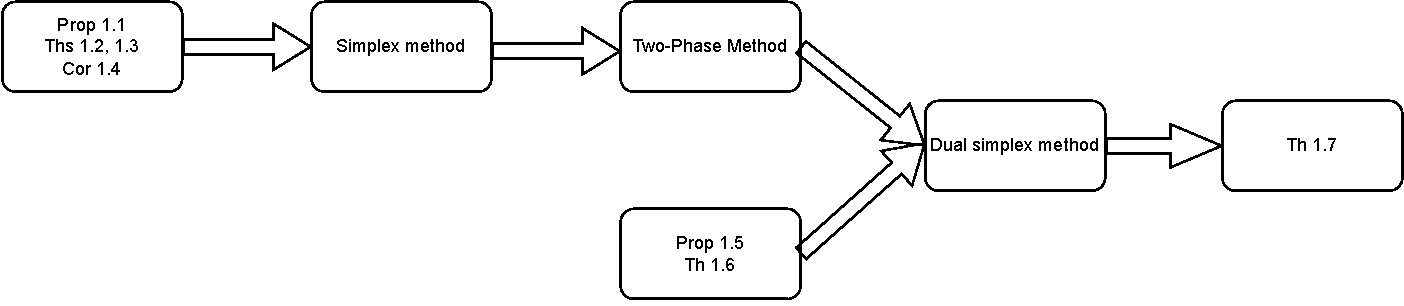
\includegraphics[scale = 0.5]{drawio1.pdf}
        \caption{The chain of implications}
        \label{fig-2}
    \end{figure}
\end{remark}

Even though the two-phase method seems stronger than the dual simplex method, we actually derived the latter from the former!

\section{Non-linear programming}
\begin{definition}
    convex: Let $X\in\mathbb{R}^n$ be convex. A function $f:X\to\mathbb{R}$ is convex if $\forall x, y\in X$ and $\lambda\in[0, 1]$
    \begin{align*}
        f\left( (1-\lambda)x+\lambda y\right)\le (1-\lambda)f(x) + \lambda f(y)
    \end{align*}
    f is strictly convex if $\forall x, y \in X$ with $x\neq y$, and $\lambda\in (0, 1)$
    \begin{align*}
        f\left( (1-\lambda)x+\lambda y\right)< (1-\lambda)f(x) + \lambda f(y)
    \end{align*}
    \begin{figure}[H]
        \centering
        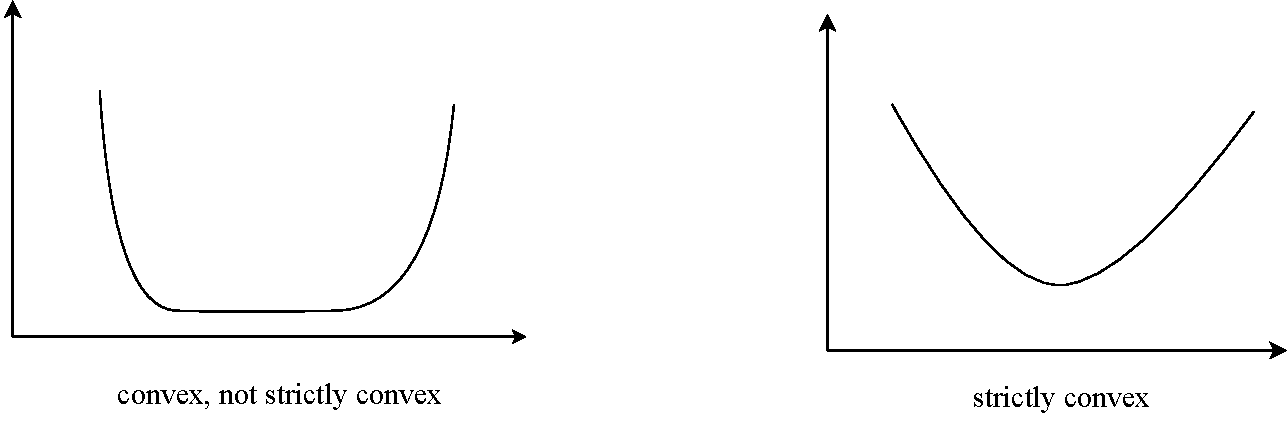
\includegraphics[scale = 0.5]{document/drawio2.pdf}
        \caption{Convex function}
        \label{fig-3}
    \end{figure}
\end{definition}

$f$ is concave/strictly concave if $-f$ is convex/strictly convex.

\begin{definition}
    Differentiable: Let $X\in\mathbb{R}^n$ be an open set. A function $f:X\to\mathbb{R}$ is $k$ times differentiable if all partial derivatives:
    \begin{align}
        \dfrac{\partial^l f}{\partial x_1^{l_1} \partial x_2^{l_2}\cdots \partial x_n^{l_n}} \label{1.13}
    \end{align}
exist, where $0\le l_i, l\le k$ and $l_1+l_2+\cdots+l_n=l$. Recall that $\dfrac{\partial^2 f}{\partial x_i\partial x_j} = \dfrac{\partial^2 f}{\partial x_j\partial x_i}$, $\forall 1\le i, j\le n$, $f$ is $k$ times continuously differentiable if in addition, all derivatives (\ref{1.13}) are continuous on $X$. If $k=1$, we omit ``$k$ times''. If $k=2$, we write ``twice'' for ``2 times''.

The gradient of $f$ is
\begin{align*}
    \nabla f(x) = \left( \frac{\partial f}{\partial x_1}, \cdots , \frac{\partial f}{\partial x_n}\right)
\end{align*}

The Hessian of $f$ is
\begin{align*}
    \left(\begin{array}{cccc}
        \frac{\partial^2 f}{\partial x_1^2} & \frac{\partial^2 f}{\partial x_1\partial x_2} & \cdots & \frac{\partial^2 f}{\partial x_1\partial x_n} \\
        \frac{\partial^2 f}{\partial x_2\partial x_1} & \frac{\partial^2 f}{\partial x_2^2} & \cdots & \frac{\partial^2 f}{\partial x_2\partial x_n} \\
        \vdots & \vdots &  & \vdots \\
        \frac{\partial^2 f}{\partial x_n\partial x_1} & \frac{\partial^2 f}{\partial x_n\partial x_2} & \cdots & \frac{\partial^2 f}{\partial x_n^2} 
    \end{array}\right),\quad \text{which is symmetric.}
\end{align*}
\end{definition}

\begin{definition}[symmetric definite matrix]
    A symmetric matrix $A\in\mathbb{R}^{n\times n}$ is:
    \item[Positive definite (正定)] Written $A>0$, if $x^TAx>0$, $\forall x\in R^n\backslash\{0\}$.
    \item[Positive semi-definite] Written $A\ge 0$, if $x^TAx\ge 0$, $\forall x\in \mathbb{R}^n$.

    The following results each characterises convex functions.
\end{definition}

\begin{theorem}
    Let $f: X\to\mathbb{R}$, where $X\subset \mathbb{R}^n$ is convex. Then $f$ is convex $\Longleftrightarrow$ $\forall x, y\in X$, $\forall \lambda\in[0, 1]$, the function:
    \begin{align*}
        h(\lambda) = f\left((1-\lambda)x + \lambda y \right)
    \end{align*}
    is convex on $\lambda\in[0, 1]$. That is, $f$ is convex when restricted to any line segment in $X$.
\end{theorem}

\begin{theorem}
    Let $f: X\to \mathbb{R}$ be differentiable, where $X\subset\mathbb{R}$ is open. Then $f$ is convex $\Longleftrightarrow$ $X$ is convex, and
    \begin{align*}
        f(y) \ge f(x) + \nabla f(x)^T(y-x)
    \end{align*}

    ``$f$ lies above the plane of contact at $x$''
\end{theorem}

\begin{theorem}
    Let $f:X\to\mathbb{R}$ be twice differentiable, where $X\subset \mathbb{R}$ is open. Then $f$ is convex $\Longleftrightarrow$ $X$ is convex, and 
    \begin{align*}
        \nabla^2 f(x) \ge 0, \quad \forall x\in Xs
    \end{align*}
\end{theorem}

The standard form of a non-linear programming problem is
\begin{align}
    \min &\quad f(x) \nonumber\\
    & g_i(x) \leqslant 0, \quad \forall 1 \leqslant i \leqslant m \label{1.14}
\end{align}
where $x \in \mathbb{R}^n$ is the optimisation variable, and $f: X_0 \rightarrow \mathbb{R}$, $g_i: X_i \rightarrow \mathbb{R}$, where $X_0, X_1, \ldots, X_m \subset \mathbb{R}^n$ are the domains of $f, g_1, \cdots, g_n$. The function $f$ is the objective function, and $g_i(x)\le 0$ are the (inequality) constraints. The domain and feasible set of problem (\ref{1.14}) are
\begin{align*}
    D& = \bigcap\limits_{i=0}^m X_i \\
    R &= \{x\in D: g_i(x)\le 0, \forall 1\le i\le m \}
\end{align*}

The \underline{optimal value} of (\ref{1.14}) is denoted by $p^*$. \underline{The optimal set} of (\ref{1.14}) is
\begin{align*}
    R^* = \{ x\in R: f(x) = p^*\}
\end{align*}

Any elements of $R^*$ is an \underline{\textcolor{MarkerColour}{\textsc{optimal solution}}}. Note that we may have $R^* = \varnothing$, even if $p^*$ is finite.
\begin{example}
    If $f(x) = e^{-x}$, then $p^* = 0$, but $R^* = \varnothing$. 

    Think of a series, its limitation isn't located on its set. Commonly appearing in Real Analysis and some courses. Secondly perhaps the function isn't continuous.
\end{example}

If $R^*\neq\varnothing$, then $p^*$ is \underline{\textcolor{MarkerColour}{\textsc{ottained}}} (by any element of $R^*$).

If $f$ and all $g_i$ in (\ref{1.14}) are convex functions (so all sets $X_i$ are convex), then (\ref{1.14}) is a \underline{\textcolor{MarkerColour}{\textsc{convex}}} \underline{\textcolor{MarkerColour}{\textsc{programming (CP) problem}}}.

\begin{theorem}
    Th 1.11 Suppose (\ref{1.14}) is a CP.

    (a) The sets $R$ and $R^*$ are convex.

    (b) If $F$ is strictly convex, and $R^*\neq \varnothing$, then $\exists$ unique optimal solution.
\end{theorem}
\begin{proof}
    (a) Let $x, y\in R$, and $\lambda\in[0, 1]$. Then $x, y\in D$ and since $D = \bigcap\limits_{i=1}^m X_i$ is convex\footnote{By HW1 in the homework}, $z=(1-\lambda)x+\lambda y\in D$. Now $1\le i\le m$, since $g_i$ is convex. Then
    \begin{align*}
        g_i(z) = g_i\left( (1-\lambda)x+\lambda y\right) \le (1-\lambda) g_i(x) + \lambda g_i(y) \le 0,
    \end{align*}
    so $z\in R$ and $R$ is convex.

    Now let $x, y\in R^*$, and $\lambda\in [0, 1]$. Then $x, y\in R$ and since $R$ is convex, we have $z = (1-\lambda)x+\lambda y\in R$. Since $f$ is convex, 
    \begin{align*}
        p^*\le f(z)= f\left( (1-\lambda)x+\lambda y\right)\le (1-\lambda)x+\lambda y = p^*
    \end{align*}

    So $f(z) = p^*$ and $z\in R^*$. Thus $R^*$ is also convex.

    (b) Suppose that $\exists$ optimal solutions $x, y\in R^*$ with $x\neq y$. Let $\lambda \in(0, 1)$. Then $(1-\lambda)x+\lambda y\in R^*$ by (a), and 
    \begin{align*}
        f\left((1-\lambda)x+\lambda y\right) < (1-\lambda)f(x)+\lambda f(y) = p^*
    \end{align*}
    a contradiction.
\end{proof}

\begin{definition}
    In problem (\ref{1.14}), $\bar{x}\in R$ is \underline{locally optimal} if $\exists\delta>0$, s.t.
    \begin{align}
        f(x) \le f(\bar{x}), \quad \forall x\in R\cap B^0(\bar{x}, \delta)\label{1.15}
    \end{align}
    where $B^0(\bar{x}, \delta) = \{ y\in \mathbb{R}^n: \|y-\bar{x}\| <\delta\}$ is the open ball with radius $\delta$, centre $\bar{x}$.
\end{definition}

\begin{remark}
    Recall that $\|z\| = \|z\|_2 = \left(\sum\limits_{i=1}^n |z_i|^2\right)^{1/2}$ is the \underline{Euclidean norm} of $z\in\mathbb{R}^n$
\end{remark}

\begin{theorem}
    Th 1.12 Suppose (\ref{1.14}) is a CP. Then $\bar{x}$ is locally optimal $\Longleftrightarrow$ $\bar{x}$ is an optimal solution.
\end{theorem}
\begin{proof}
    Clearly it suffices to prove $\left(\Longrightarrow\right)$. Let $\bar{x}$ be locally optimal. Then $\bar{x}$ satisfies (\ref{1.15}) for some positive $\delta > 0$. Suppose $\bar{x}\notin R^*$, so $\exists y\in R$, $y\neq \bar{x}$, s.t. $f(y)<f(\bar{x})$. Then $\| y-\bar{x}\| \ge \delta$. Choose $z$ where 
    \begin{align*}
        z = (1-\lambda)x + \lambda y, \quad \lambda = \dfrac{\delta}{2\|y-\bar{x}\|}.
    \end{align*}

    Then $\|z-\bar{x}\| = \frac{\delta}{2} < \delta$. Since $R$ is convex by Th 1.11(a), $z\in R$. Since $f$ is convex, 
    \begin{align*}
        f(z) = f\left( (1-\lambda)\bar{x} + \lambda y\right) \le (1-\lambda) f(\bar{x}) + \lambda f(y) = f(\bar{x}) + \lambda\left(f(y) - f(\bar{x})\right) < f(\bar{x}).
    \end{align*}
    which contradicts (\ref{1.15}). Thus $\bar\in R^*$.
\end{proof}

\begin{theorem}
    Th 1.13 Suppose that (\ref{1.14}) is a CP, where $f$ is differentiable. Then $\bar{x}\in R^* \Longleftrightarrow \bar{x}\in R$, and
    \begin{align}
        \nabla f(\bar{x})^T (y-\bar{x}) \ge 0, \quad \forall y\in R.\label{1.16}
    \end{align}
\end{theorem}

\begin{proof}
    $\Longleftarrow$ 
    
    \noindent Suppose $\bar{x}\in R$ and satisfies (\ref{1.16}). If $y\in R$, then 
    \begin{align*}
        f(y) \underset{\text{Th 1.9}}{\ge} f(\bar{x}) + \nabla f(\bar{x})^T (y-\bar{x}) \underset{(\ref{1.16})}{\ge} f(\bar{x}),
    \end{align*}
    so $\bar{x}$ is optimal.

    $\Longrightarrow$ 
    
    \noindent Suppose $\bar{x}\in R^*$. Then $\bar{x}\in R$. Suppose (\ref{1.16}) is false. Then $\exists y\in R$ s.t. $\nabla f(\bar{x})^T (y-\bar{x}) < 0$. Consider $z(\lambda) = (1-\lambda)\bar{x} +\lambda y$, where $\lambda\in(-\varepsilon, 1-\varepsilon)$ for some small $\varepsilon>0$. By Th 1.11(a), $R$ is convex, so $z(\lambda)\in R$. Now
    \begin{align*}
        \frac{d}{d\lambda} f\left( z(\lambda)\right) &\underset{\textsc{Chain rule}}{=} Df(z(\lambda))Dz(\lambda) = \nabla f(z(\lambda))^T (y-\bar{x}) \\
        \frac{d}{d\lambda}\bigg|_{\lambda=0} &= \nabla f(\bar{x})^T (y-\bar{x}) < 0
    \end{align*}
    so if $\lambda>0$ is sufficiently small, then $f(z(\lambda)) < f(z(0)) = f(\bar{x})$. Thus $\bar{x}\notin R^*$, a contradiction.
\end{proof}

\begin{theorem}
    Th 1.14 Suppose that (\ref{1.14}) is a CP and is unconstrained, that is, $m = 0$. Let $f$ be differentiable. Then $\bar{x}\in R^* $ \quad $\Longleftrightarrow$ \quad $\nabla f(\bar{x}) = 0$.
\end{theorem}
\begin{proof}
    \par
    ($\Longrightarrow$) Let $\bar{x}\in R^*$. Then Th 1.13 $\Longrightarrow$ $\nabla f(\bar{x})^T(y-\bar{x}) \ge 0$, $\forall y\in R$. Since $f$ is differentiable, $\exists$ open neighborhood $U$ of $\bar{x}$, s.t. $\forall y\in U$, we have $y\in R$. Let $y = \bar{x} - t\nabla f(\bar{x})$ where $t>0$ is small, and $y\in R$. Then
    \begin{align*}
        0 \le \nabla f(\bar{x})^T (y-\bar{x}) = -t \|\nabla f(\bar{x})\|^2,
    \end{align*}
    where implies $\nabla f(\bar{x}) = 0$.
    \par
    ($\Longleftarrow$) Suppose $\nabla f(\bar{x}) = 0$. Clearly $\bar{x}\in X_0$, so $\bar{x}\in R$. Also, $\nabla f(\bar{x})^T(y-\bar{x}) = 0$, $\forall y\in R$. Thus TH 1.13 $\Longrightarrow$ $\bar{x}$ is optimal.
\end{proof}

\subsection{Duality and the Lagrangian}
Given problem (\ref{1.14}). suppose the domain $D\neq \varnothing$. We define the  \underline{\textcolor{MarkerColour}{\textsc{Lagrangian}}} $L: D\times\mathbb{R}^m \to \mathbb{R}$ by
\begin{align*}
    L(x, \lambda) = f(x) + \sum\limits_{i=1}^m \lambda_i g_i(x)
\end{align*}

\begin{definition}
    The \underline{\textcolor{MarkerColour}{\textsc{Lagrange dual function}}} is defined by
    \begin{align}
        h(\lambda) = \inf\limits_{x\in D} L(x, \lambda) = \inf\limits_{x\in D} \left(f(x) + \sum\limits_{i=1}^m \lambda_i g_i(x) \right) \nonumber
    \end{align}

    The \underline{\textcolor{MarkerColour}{\textsc{(Lagrange) dual problem}}} of (\ref{1.14}) is 
    \begin{align}
        \max\quad & h(\lambda)\nonumber \\
        & \lambda \ge 0\label{1.17}
    \end{align}
    where $\lambda\in\mathbb{R}^m$ is a variable. Let $d^*$ denote the optimal value of problem (\ref{1.17}). If $h(\bar{\lambda}) = d^*$ for some $\bar{\lambda}\in\mathbb{R}^m$, $\lambda\ge 0$, then $d^*$ is  \underline{\textcolor{MarkerColour}{\textsc{attained}}} (by $\bar{\lambda})$, and $\bar{\lambda}$ is an \underline{\textcolor{MarkerColour}{\textsc{optimal solution}}} of (\ref{1.17}). We also call (\ref{1.14}) the \underline{\textcolor{MarkerColour}{\textsc{primal problem}}}.
\end{definition}

\begin{theorem}
    Th 1.15 \underline{\textcolor{MarkerColour}{\textsc{Weak Duality}}}
    \par Suppose problem (\ref{1.14}) has an optimal value $p^*$. Then $\forall \lambda\in\mathbb{R}^m$, $\lambda\ge 0$, 
    \begin{align*}
        p^* \ge h(\lambda)
    \end{align*}

    Thus, $p^*\ge d^*$. This property is \underline{\textcolor{MarkerColour}{\textsc{Weak Duality}}} between problems (\ref{1.14}) and (\ref{1.17}). 
\end{theorem}
\begin{proof}
    The result holds if $h(\lambda) = -\infty$ or $p^* = \infty$, so assume otherwise. Then $R\neq\varnothing$. Let $y\in R$ in (\ref{1.14}), so $g_i(y)\le 0$, $\forall 1\le i\le m$. Then for $\lambda\in\mathbb{R}^m$, $\lambda\ge 0$,
    \begin{align*}
        h(\lambda) = \inf\limits_{x\in D} L(x, \lambda) \le L(y, \lambda) = f(y) + \sum\limits_{i=1}^m \lambda_i g_i(y) \le f(y).
    \end{align*}

    Since $h(\lambda) \le f(y)$. $\forall y\in R$, we have $h(\lambda) \le p^*$.
\end{proof}

If $p^* = d^*$, then we have \underline{\textcolor{MarkerColour}{\textsc{Strong duality}}} between problems (\ref{1.14}) and (\ref{1.17}). We do not always have strong duality, even if (\ref{1.14}) is a CP.

We can show that the Lagrange dual problem of the LP (\ref{LP-3}) is the dual LP (\ref{dual LP})\footnote{HW 2 problem}.

\subsection{KT conditions}
We will see that under some conditions, we have a necessary and sufficient condition for \underline{\textcolor{MarkerColour}{\textsc{Strong duality}}} between (\ref{1.14}) and (\ref{1.17}).

\begin{theorem}
    \textsc{Th 1.16} \underline{\textcolor{MarkerColour}{\textsc{Kuhn-Tucker Theorem}}}
    \par We have the primal problem (\ref{1.14}) and its dual problem (\ref{1.17}).

    (a) Suppose that the optimal values $p^*$ of (\ref{1.14}) and $d^*$ of (\ref{1.17}) are both attained, and we have strong duality $p^* = d^*$. Let $\bar{x}$ and $\bar{\lambda}$ be optimal solutions. Then
    \begin{align}
        \begin{array}{rlll}
             g_i(\bar{x})\le 0, & 1\le i\le m & \text{Primal feasible} & \text{(1.18 a)} \\
            \bar{\lambda}_i \ge 0, & 1\le i\le m & \text{Dual feasible} & \text{(1.18 b)}\\
            \bar{\lambda}g_i(\bar{x}) = 0 & 1\le i\le m & \text{Complementary slacks} & \text{(1.18 c)}
        \end{array}\label{1.18}
    \end{align}

    If in addition, $f$ and $g$, $(1\le i\le m)$ are differentiable (so the domains $X_i (0\le i\le m)$ are open), then
    \begin{align*}
        \begin{array}{lll}
            \nabla f(\bar{x}) + \sum\limits_{i=1}^m \bar{\lambda}_i \nabla g_i(\bar{x}) = 0 & \text{Stationary condition} & \text{(1.18 d)}
        \end{array}
    \end{align*}

    (b) Conversely, suppose that (\ref{1.14}) is a CP, and $f$ and $g_i (1\le i\le m)$ are differentiable. If $\bar{x}$ and $\bar{\lambda}$ satisfy the conditions (1.18 a-d), then $\bar{x}$ and $\bar{\lambda}_i$ are optimal solutions yielding strong duality $p^* = d^*$.

    The condition (1.18 a-d) are the KT conditions.
\end{theorem}
\begin{proof}
    (a) Clearly (1.18 a, b) hold. Now, 
    \begin{align*}
        f(\bar{x}) = h(\bar{\lambda}) &= \inf\limits_{x\in D} L(x, \bar{\lambda}) \le L(x, \bar{\lambda}) \\
        & = f(\bar{x}) + \sum\limits_{i=1}^m \bar{\lambda}_i g_i(\bar{x}) \le f(\bar{x})
    \end{align*}
    so equality holds throughout. We have $\sum\limits_{i=1}^m \bar{\lambda}_i g_i(\bar{x}) = 0$ and (1.18 a-b) $\Rightarrow$ $\bar{\lambda}_i h_i(\bar{x}_i)\le 0\quad (1\le i\le m)$, so (1.18 c) holds. 

    Also $\bar{x}$ minimises $L(x, \bar{\lambda})$. Suppose $f$ and $g_i\quad(1\le i\le m)$ are differentiable. Then $\nabla_x L(\bar{x}, \bar{\lambda}) = 0$, which is (\ref{1.18} d).

    (b) Since $L(x, \bar{\lambda})$ is a sum of convex functions in $x$, $L(x, \bar{\lambda})$ is convex in $x$\footnote{HW 2}. Since (\ref{1.18} d) says $\nabla_x L(\bar{x}, \bar{\lambda}) = 0$, Th 1.14$\Rightarrow$ $\bar{x}$ minimises $L(x, \bar{\lambda})$. Thus, 
    \begin{align*}
        h(\bar{\lambda}) = L(\bar{x}, \bar{\lambda}) = f(\bar{x}) + \sum\limits_{i=1}^m \bar{\lambda}_i g_i(\bar{x}) \underset{\text{(\ref{1.18} c)}}{=} f(\bar{x}).
    \end{align*}

    Thus $\bar{x}$ and $\bar{\lambda}$ are optimal solutions. and $p^* = d^*$.
\end{proof}

\begin{remark}
    $\nabla_x$ means $\nabla$ is taken w.r.t $x$.
\end{remark}

\begin{example}
    Solve the CP 
    \begin{align}
        \min &\quad f(x_1, x_2) = (x_1 - 6)^2 + (x_2 - 5)^2 \nonumber \\
        & \left\lbrace  \begin{array}{rl}
        x_1^2 -2x_1+x_2 &\le 8  \\
        x_1,x_2 &\ge 0
        \end{array} \label{1.19}\right.
    \end{align}

    By Th 1.16, the solution to (\ref{1.19}) is achieved by any $\bar{x}$, $\bar{\lambda}$ satisfying the KT conditions (\ref{1.18}). We have:
    \begin{align}
        \label{1.20}\left\lbrace\begin{array}{ll}
            g_1(x_1, x_2) = x_1^2 - 2x_2 +x_2 - 8 \le 0 & \text{(\ref{1.20} a)} \\
            g_2(x_1, x_2) = -x_1 \le 0 & \text{(\ref{1.20} a')}\\
            g_3(x_1, x_2) = -x_2 \le 0 & \text{(\ref{1.20} a'')}
        \end{array}\right.  \\
        \begin{array}{ll}
             \lambda_1, \lambda_2, \lambda_3\ge 0 & \text{(\ref{1.20} b)} \nonumber \\
            \lambda_1(x_1^2-2x_1+x_2-8) = \lambda_2 x_1 = \lambda_3 x_2 = 0 & \text{(\ref{1.20} c)}
        \end{array} \\
        \left(\begin{array}{c}
            2(x_1-6) + \lambda_1(2x_2-2) -\lambda_2  \\
            2(x_2 - 5) + \lambda_1 - \lambda_3 
        \end{array} \right) = \left( \begin{array}{c}
             0 \\
             0 
        \end{array}\right) \quad \quad \text{(\ref{1.20} d)}\nonumber
    \end{align}

    Solving this, we have $\bar{x}_1 = \frac{3+\sqrt{11}}{2}$, $\bar{x}_2 = \frac{12-\sqrt{11}}{2}$, $\lambda_1 = \sqrt{11} - 2$, $\lambda_2 = \lambda_3 = 0$. The minimum value of $f$ is:
    \begin{align*}
        (\bar{x}_1 - 6)^2 + (\bar{x}_2 - 5)^2 = \left(\frac{-9 + \sqrt{11}}{2}\right)^2 + \left(\frac{2-\sqrt{11}}{2}\right)^2 = \frac{107-22\sqrt{11}}{4}
    \end{align*}
\end{example}

The detailed calculations is following:

Case 1. $\lambda_{1}=0$.

By $(1.20 \mathrm{~d})$, we have $2\left(x_{1}-6\right)=\lambda_{2}$ and $2\left(x_{2}-5\right)=\lambda_{3}$. Then by $(1.20 \mathrm{~b}, \mathrm{c})$, we have $x_{1}=6, \lambda_{2}=0$, and $x_{2}=5, \lambda_{3}=0$. But then $g_{1}(6,5)=21$, and (1.20a) does not hold. Thus we cannot have the case $\lambda_{1}=0$.

Case 2. $\lambda_{1}>0$.

By (1.20 c), we have $x_{1}^{2}-2 x_{1}+x_{2}-8=0$. If $x_{1}=0$, then (1.20d) gives $2 \lambda_{1}+\lambda_{2}=-12$, which contradicts $(1.20 \mathrm{~b})$. So $x_{1}>0$, and (1.20c) implies $\lambda_{2}=0$. Then if $x_{2}=0$, we have $0=x_{1}^{2}-2 x_{1}-8=\left(x_{1}-4\right)\left(x_{1}+2\right)$, so $x_{1}=4$. By (1.20d), we have $-4+6 \lambda_{1}=0$ and $-10+\lambda_{1}-\lambda_{3}=0$, which gives $\lambda_{1}=\frac{2}{3}$, and $\lambda_{3}=-10+\frac{2}{3}<0$, contradicting (1.20b). So $x_{2}>0$, and (1.20c) implies $\lambda_{3}=0$. Now (1.20d) gives $2\left(x_{1}-6\right)+\lambda_{1}\left(2 x_{1}-2\right)=0$ and $2\left(x_{2}-5\right)+\lambda_{1}=0$. Eliminating $\lambda_{1}$ and using $x_{2}=8-x_{1}^{2}+2 x_{1}$, we have $x_{1}\left(2 x_{1}^{2}-6 x_{1}-1\right)=0$. Solving the quadratic gives $\bar{x}_{1}=\frac{3+\sqrt{11}}{2}$, and then easy calculations give $\bar{x}_{2}=\frac{12-\sqrt{11}}{2}$ and $\bar{\lambda}_{1}=\sqrt{11}-2$. We already know that $\bar{\lambda}_{2}=\bar{\lambda}_{3}=0$. This is the unique optimal solution, and the optimal value of $f$ is
\begin{align*}
    \left( \bar{x}_{1}-6\right)^{2} + \left(\bar{x}_{2}-5\right)^{2} = \left(\frac{-9+\sqrt{11}}{2}\right)^{2}+\left(\frac{2-\sqrt{11}}{2}\right)^{2}=\frac{107-22 \sqrt{11}}{4} .
\end{align*}

\subsection{Algorithm Methods}
In general, problem (\ref{1.14}) can't be solved exactly. We consider algorithm methods we can give approximate solutions to (\ref{1.14}).

We first consider the case when (\ref{1.14}) is an unconstrained CP. That is:
\begin{align}
    \min &\quad f(x) \label{1.21} 
\end{align}
where $f: X\to\mathbb{R}$ is a convex function, for some convex $X\subset \mathbb{R}^n$. Suppose $f$ is twice continuously differentiable, so $X$ is open, and (\ref{1.21}) has an optimal solution $\bar{x}$. Suppose $x^{(0)}\in X$ and $x^{(0)}\notin R^*$. We iteratively find $x^{(0)}, x^{(1)}, x^{(2)}, \cdots\in X$, s.t. $f(x^{(k)}\to p^*$ as $k\to\infty$. Such $\{x^{(k)}\}_{k=0}^{\infty}$ is a \underline{\textcolor{MarkerColour}{\textsc{minimising sequence}}}. We end the algorithm when some form of accuracy is achieved. The set
\begin{align*}
    S = \{x\in X: f(x) \le f(x^{(n)} \}
\end{align*}
is convex\footnote{In HW1}. Suppose $S$ is compact. We want to find the $x^{(k)}$ s.t.
\begin{align*}
    f(x^{(0)}) > f(x^{(1)}) > \cdots > p^*
\end{align*}

Such an algorithm is a \underline{\textcolor{MarkerColour}{\textsc{descent method}}}. We have $x^{(k)}\in S$, $\forall k>0$. Each iteration involves a direction $z^{(k)}\in \mathbb{R}^n$ and a step size $t^{(k)}\ge 0$. Thus
\begin{align*}
    x^{(k+1)} = x^{(k)} + t^{(k)}z^{(k)},
\end{align*}
or
\begin{align*}
    x^+ = x + tz
\end{align*}
if we want to focus on one iteration.

Th 1.8 $\Rightarrow$ $f$ is convex on the line segment $L = \{x+\lambda z:\lambda\ge 0 \}$, and $f\bigg|_L$ attains its minimum in $L$. We usually choose 
\begin{align}
    t \in \{\lambda\ge 0: f(x+\lambda z)\text{ is minimised on $L$ at $\lambda$} \}.\label{1.22}
\end{align}
We remark that there are other choices for $t$, since (\ref{1.22}) is not always easy to compute.

We consider two possible choices for the direction $z$.

\noindent\underline{\textcolor{MarkerColour}{\textsc{A. Steepest Descent Method}}}

We choose $z = -\nabla f(x)$. Th 1.14 $\Rightarrow$ $\nabla f(x)\neq 0$, since $x\notin R^*$. For small $\lambda>0$, 
\begin{align*}
    f(x^*) &= f(x+tz) \le f(x+\lambda z) = f(x) + \lambda \nabla f(x)^T z + o(\lambda) \\
    &= f(x) - \lambda \|\nabla f(x)\|^2 + o(\lambda) < f(x),
\end{align*}
where $o(\lambda)$ means that $\frac{0(\lambda)}{\lambda}\to 0$ as $\lambda\to 0$. So $z = -\nabla f(x)$ is a suitable choice.

\noindent\underline{\textcolor{MarkerColour}{\textsc{B. Newton's Method}}}

Assume $\nabla^2 f(x) > 0$, $\forall x\in S$. Note that $\nabla^2 f(x)$ is invertible. Taylor's theorem $\Rightarrow$
\begin{align*}
    f(x+v) \approx f(x) + \nabla f(x)^T v + \frac{1}{2} v^T \nabla^2 f(x) v = \hat{f}(x+v)
\end{align*}
$\hat{f}(x+v)$ is a convex quadratic function in $v$, minimised at $v = \nabla^2 f(x)^{-1}\nabla f(x)$\footnote{HW 2}. We define the \underline{\textcolor{MarkerColour}{\textsc{Newton Step}}}:
\begin{align*}
    z = -\nabla^2 f(x)^{-1} \nabla f(x).
\end{align*}

\begin{figure}[H]
    \centering
    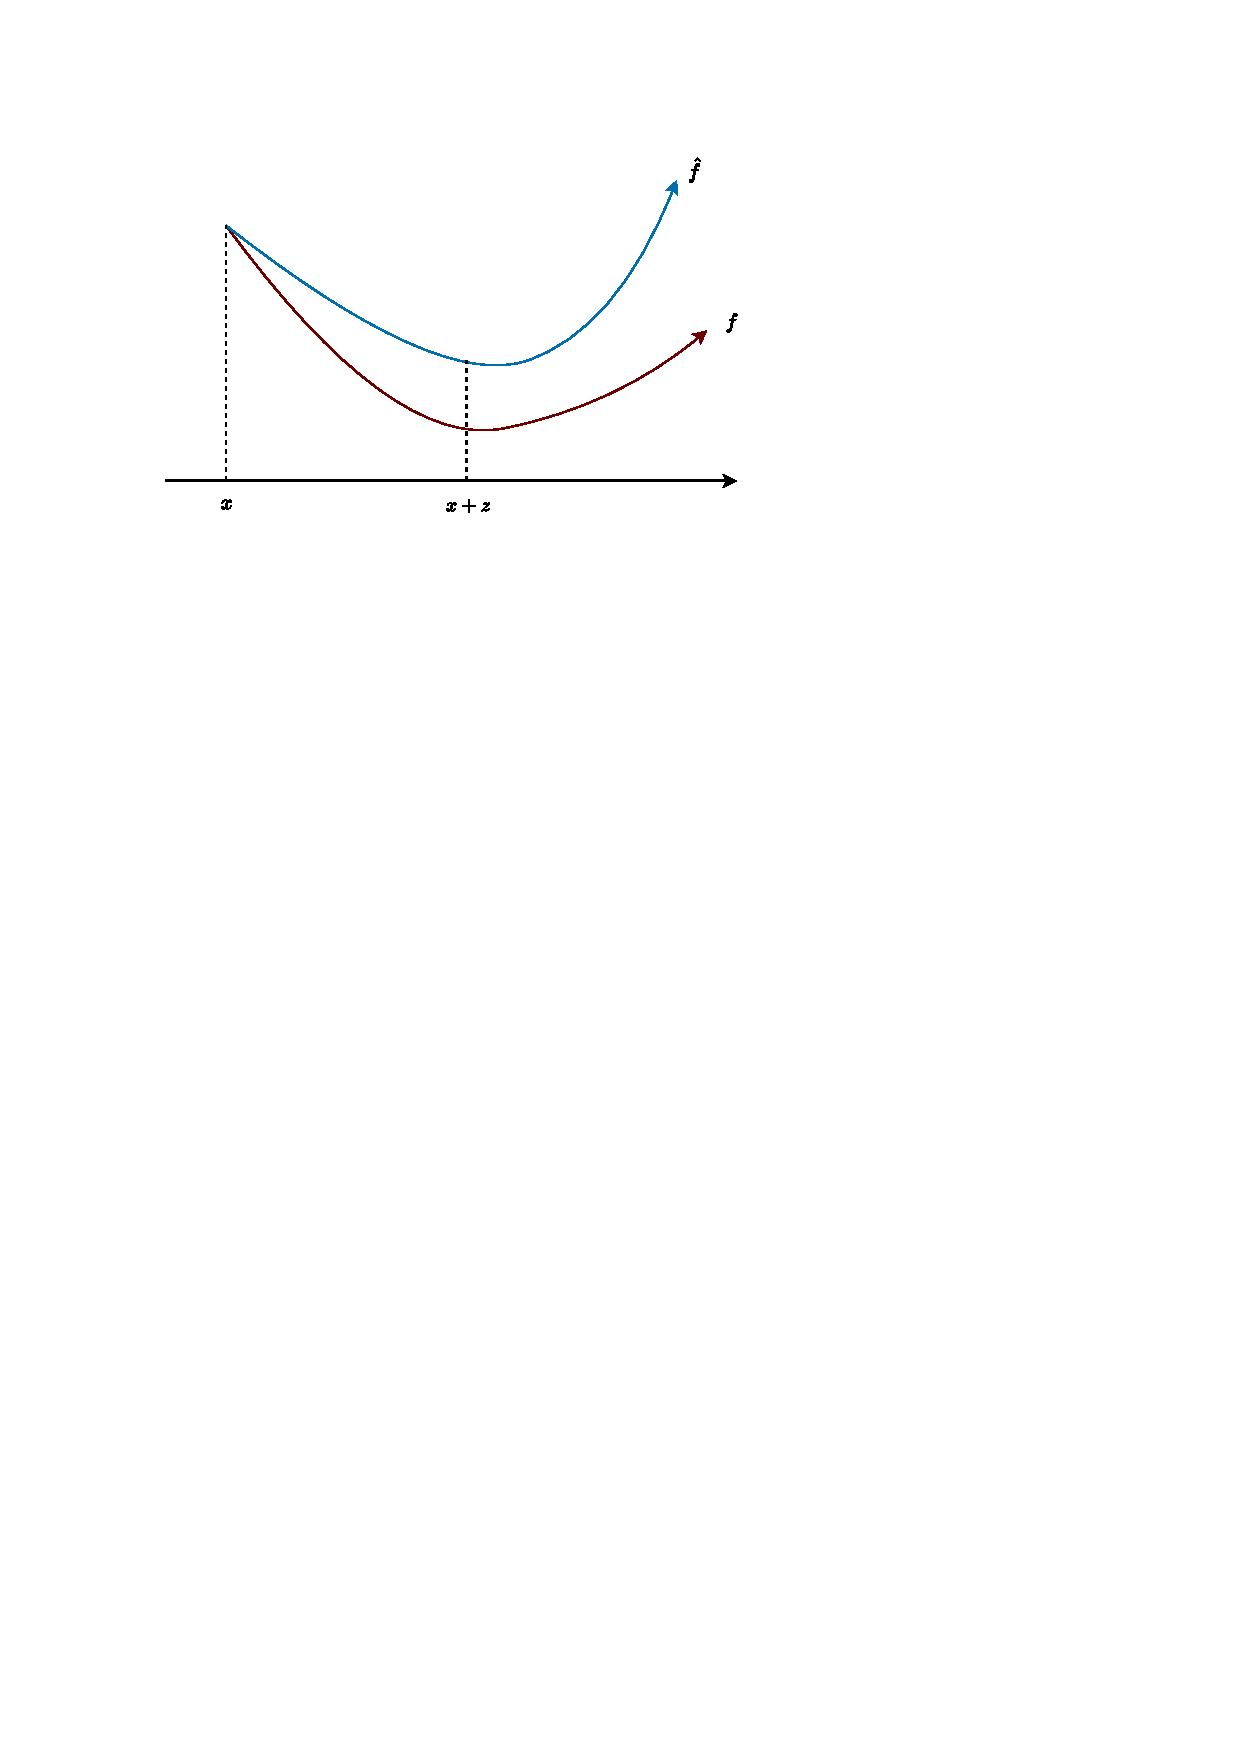
\includegraphics[scale = 0.8, trim={0cm, 20cm, 7cm, 3cm}, clip]{document/operation_1.drawio.pdf}
\end{figure}

For small $\lambda>0$,
\begin{align*}
    f(x^+) & = f(x+tz) \le f(x+\lambda z) = f(x) + \lambda\nabla f(x)^Tz + o(\lambda) \\
    &= f(x) - \lambda \nabla f(x)^T \nabla^ f(x)^{-1}\nabla f(x) + o(\lambda) < f(x),
\end{align*}
since $\nabla^2 f(x)^{-1}>0$. So $z = -\nabla^2 f(x)^{-1} \nabla f(x)$ is a suitable choice.

$f(x) = o(g(x))$ means $\frac{f(x)}{g(x)}\to 0$ as $x\to c$ for some $c$. In most cases, $c= \infty$ or $c = 0$. 

Note: ``$o$ \uuline{depends on} $c$''

Thus, we have the following algorithm for solving (\ref{1.21}). Fix $\varepsilon>0$. Suppose we found $x^{(0)}, x^{(1)}, \cdots, x^{(k)}\in S$. We find $z$ using $A$ or $B$ above. $A$ stopping criteria can be $\|z^{(k)}\|\leqslant \varepsilon$. If $\|z^{(k)}\|\geqslant \varepsilon$, thus we find $x^{(k+1)}$, and iterate.

\begin{example}
    Consider
    \begin{align*}
        \min &\quad f(x_1, x_2) = x_1^4 + 8x_2^4 \\
    \end{align*}
    where $(x_1, x_2)\in \mathbb{R}^2$. We have $p^* = 0$, where $(x_1, x_2) = (0, 0)$. Suppose we use the above algorithm with $\varepsilon = 0.1$ $x^{(0)}=\left(\begin{array}{l}2 \\ 1\end{array}\right)$. For steepest descent method, we have
\begin{align*}
\begin{gathered}
\nabla f(x)=\left(\begin{array}{l}
4 x_1^3 \\
32 x_2^3
\end{array}\right), z^{(0)}=-\nabla f\left(x^{(0)}\right)=-\left(\begin{array}{l}
32 \\
32
\end{array}\right) \\
f(2-32 \lambda, 1-32 \lambda)=(2-32 \lambda)^4+8(1-32 \lambda)^4 \\
\frac{d f}{d \lambda}=-128(2-32 \lambda)^3-1024(1-32 \lambda)^3
\end{gathered}
\end{align*}

    Solving $\frac{d f}{d \lambda}=0 \Rightarrow t^{(0)}=\frac{1}{24}$. Thus, $x^{(1)}=\left(\begin{array}{l}2 \\ 1\end{array}\right)-\frac{1}{24}\left(\begin{array}{c}32 \\ 32\end{array}\right)=\left(\begin{array}{c}\frac{2}{3} \\ -\frac{1}{3}\end{array}\right)$. We have $z^{(1)}=-\nabla f\left(x^{(1)}\right)=\left(\begin{array}{c}-\frac{32}{27} \\ \frac{32}{27}\end{array}\right)$ and $\left\|z^{(1)}\right\|=\frac{32}{27} \sqrt{2}>\varepsilon$. We iterate this until we find $z^{(k)}$ with $\left\|z^{(k)}\right\|<\varepsilon=0.1$.

    For Newton's method, we have:
    \begin{align*}
        \nabla^2 f(x)=\left(\begin{array}{cc}
        12 x_1^2 & 0 \\
        0 & 96 x_2^2
        \end{array}\right)&, \quad \nabla^2 f(x)^{-1}=\left(\begin{array}{cc}
            \frac{1}{12 x_1^2} & 0 \\
            0 & \frac{1}{96 x_2^2}
        \end{array}\right)\\
        -\nabla^2 f(x)^{-1} \nabla f(x)=-\left(\begin{array}{cc}\frac{1}{12 x_1^2} & 0 \\ 0 & \frac{1}{96 x_2^2}\end{array}\right)\left(\begin{array}{c}4 x_1^3 \\ 32 x_2^3\end{array}\right)=-\left(\begin{array}{c}\frac{x_1}{3} \\ \frac{x_2}{3}\end{array}\right)&, z^{(0)}=-\left(\begin{array}{c}
             \frac{2}{3}  \\
             \frac{1}{3}
        \end{array}\right)
    \end{align*}

    Thus $f(2-\frac{2}{3}\lambda, 1 - \frac{1}{3}\lambda) = (2- \frac{2}{3}\lambda)^4 + 8(1-\frac{1}{3}\lambda)^4 = 24(1-\frac{1}{3}\lambda)^4$, which is minimised at $\lambda = 3$. So $t^{(0)} = 3\Longrightarrow x^{(1)} = \left(\begin{array}{c}
         2  \\
         1 
    \end{array}\right) - 3\left(\begin{array}{c}
         \frac{2}{3}  \\
         \frac{1}{3}
    \end{array}\right) = \left(\begin{array}{c}
         0  \\
         0 
    \end{array}\right)$, and we terminate in one step.
\end{example}

\uline{\textcolor{MarkerColour}{\textsc{Penalty function Method}}}

Again, consider problem (\ref{1.14}), with $f$ and $g_i(1\le i\le m)$ continuous. We introduce the \uline{penalty program}, which is the unconstrained problem:
\begin{align}
    \min&\quad q(c, x) = f(x) + cp(x) \label{1.23}
\end{align}
over $x\in \mathbb{R}^n$, where $c>0$, and $p:\mathbb{R}^n\to\mathbb{R}$ is the \uline{penalty function}, s.t. $p$ is continuous, $p(x)\ge 0$, $\forall x\in\mathbb{R}^n$ and $p(x) = 0\Longleftrightarrow x\in R$. The \uline{penalty term} $cp(x)$ gives a cost if $x$ violates the constraints of (\ref{1.14}).

\begin{remark}
    Recall: If $f:X\to \mathbb{R}$, where $X\subset \mathbb{R}^n$, then
    \begin{align*}
        \underset{x\in X}{\arg \min} f(x) = \{ y\in X: f(y)\leqslant f(x), \forall x\in X\}.
    \end{align*}
\end{remark}

\begin{lemma}
    Let $0<c_1<c_2<\cdots$ with $c_k\to\infty$. Let $q(c, x) = f(x) + cp(x)$ as in (\ref{1.23}). Let $x_k\in\underset{x\in\mathbb{R}^n}{\arg\min} q(c_k, x)$. Then $\forall k\geqslant 1$,\footnote{Proof HW2}
    \begin{align*}
        (a) & q(c_k, x_k) \leqslant q(c_{k+1}, x_{k+1}).\\
        (b) & p(x_k) \geqslant p(x_{k+1}) \\
        (c) & f(x_k) \leqslant f(x_{k+1}) \\
        (d) & f(x^*) \geqslant q(c_k, x_k) \geqslant f(x_k), \quad \text{where } x^*\in R^* (\text{of problem (\ref{1.14})}).
    \end{align*}
\end{lemma}

\begin{remark}
    Recall: For $S\subset \mathbb{R}^n$, a \uline{limit point} of $S$ is $x\in\mathbb{R}^n$ s.t.

    $\forall$ open set $U$ with $x\in U$, $\exists y\in S\backslash\{x\}$, s.t. $y\in U$.
\end{remark}

\begin{theorem}
    With the same notations as in (\ref{1.23}) and Lemma 1.17, let $\bar{x}$ be a limit point of $\{x_k\}_{k=1}^{\infty}$. Then $\bar{x}\in R^*$ in problem (\ref{1.14}). 
\end{theorem}
\begin{proof}
    Take a sub-sequence $x_{k_1}, x_{k_2}, \cdots$ of $\{x_k\}_{k=1}^{\infty}$ s.t. $x_{k_j}\to \bar{x}$\footnote{HW 2}. Since $f$ and $p$ are continuous, 
    \begin{align*}
        &\bar{q} = \lim\limits_{k_j\to \infty} q(c_{k_j}, x_{k_j}) = \lim\limits_{k_j\to\infty} f(x_{k_j}) + \lim\limits_{k_j\to\infty} c_{k_j} p(x_{k_j}) \underset{\text{Th 1.17(d)}}{\leqslant} f(x^*) \\
        \Longrightarrow & \bar{q} - f(\bar{x}) = \lim\limits_{{k_j}\to\infty} c_{k_j}p(x_{k_j}) \leqslant f(x^*) - f(\bar{x})
    \end{align*}

    Thus $\lim\limits_{k_j\to\infty} c_{k_j}p(x_{k_j})$ is finite, and since $c_{k_j}\to\infty$, we have $p(x_{k_j})\to 0$. Thus $p(\bar{x}) = 0$, and $\bar{x}\in R$. Moreover, 
    \begin{align*}
        &f(x^*) \geqslant f(\bar{x}) + \lim\limits_{k_j\to\infty} c_{k_j} p(x_{k_j}) \geqslant f(\bar{x}) \\
        \Longrightarrow & f(x^*) = f(\bar{x}), \quad \text{and } \bar{x}\in R^*
    \end{align*}
\end{proof}

A commonly used penalty function is 
\begin{align}
    p(x) = \sum\limits_{i=1}^m \left[ \max(0, g_i(x))\right]^t, \quad \text{for some } t\geqslant 1.\label{1.24}
\end{align}
Especially, the cast $t=2$.

Suppose (\ref{1.14}) also has equality constraints:
\begin{align}
    \min &\quad f(x) \nonumber \\
    & \left\lbrace\begin{array}{ll}
    g_i(x) \leqslant 0, & 1\leqslant i\leqslant m \\
    h_i(x) = 0 & 1\leqslant i\leqslant r 
    \end{array} \right.\label{1.25}
\end{align}
where $h_i:Y_i\to\mathbb{R}$, with $Y_i\subset \mathbb{R}^n$ the domain of $h_i$. We may rewrite (\ref{1.25}) in the form of (\ref{1.14}).
\begin{align*}
    \min &\quad f(x) \nonumber \\
    & \left\lbrace\begin{array}{rl}
    g_i(x) \leqslant 0, & 1\leqslant i\leqslant m \\
    h_i(x) \leqslant 0 & 1\leqslant i\leqslant r \\
    -h_i(x) \leqslant 0 & 1\leqslant i\leqslant r 
    \end{array} \right. 
\end{align*}
and work from there. The penalty function (\ref{1.24}) becomes
\begin{align}
    p(x) = \sum\limits_{i=1}^m \left[ \max(0, g_i(x)) \right]^t + \sum\limits_{i=1}^r \left| h_i(x) \right|^t \label{1.26}
\end{align}

\begin{example}
    Use the penalty function method to solve
    \begin{align*}
        \min &\quad -3x_1 + x_2 \\
        & x_1^2 - 2x_2 \leqslant 4
    \end{align*}
\end{example}

From (\ref{1.23}) and (\ref{1.26}) with $t = 2$, we have
\begin{align*}
    q(c_k, x) = \left\lbrace\begin{array}{ll}
         -3x_1 + x_2  & \text{if } x_1^2 - x_2 - 4\leqslant 0 \\
         -3x_1 + x_2 + c_k\left(x_1^2 - x_2 - 4\right)^2 & \text{if } x_1^2 - x_2 - 4 > 0
    \end{array} \right.
\end{align*}

We find $x_k\in\underset{x\in\mathbb{R}^n}{\arg\min} q(c_k, x)$.
\begin{itemize}
    \item If $x_1^2 - 2x_2 - 4\leqslant 0$, then $-3x_1 + x_2 \leqslant \frac{1}{2}x_1^2 - 3x_2 - 2 = \frac{1}{2}\left(x_1 - 3\right)^2\geqslant -\frac{13}{2}$, with equality when $(x_1, x_2) = (3, \frac{5}{2})$. Minimum $q(c_k, x) = -3\cdot 3 + \frac{5}{2} = -\frac{13}{2}$
    \item If $x_1^2 - 2x_2 - 4>0$. We solve $\nabla_x q(c_k, x) = 0$ (See Th 1.14). We have 
    \begin{align*}
        \nabla_x q(c_k, x) = \left(\begin{array}{c}
             -3+4c_k x_1(x_1^2 - 2x_2 -4)  \\
             1 - 4c_k(x_1^2 - 2x_1 -4)
        \end{array}\right) = \left(\begin{array}{c}
             0  \\
             0 
        \end{array} \right). 
    \end{align*}
    We can find $x_1 = 3$, $x_2 = \frac{5}{2} - \frac{1}{8c_k}$, and minimum $q(c_k, x) = -\frac{13}{2} - \frac{1}{16c_k}$. Thus $x_k = (3, \frac{5}{2} - \frac{1}{8c_k}\to (3, \frac{5}{2})$. Th 1.18
\end{itemize}
\begin{align*}
    \Longrightarrow \bar{x} = (3, \frac{5}{2})\in R^*, \text{and } p^* = -3\cdot 3 + \frac{5}{2} = -\frac{13}{2}
\end{align*}

\begin{example}
    Use the penalty program method to solve
    \begin{align*}
        \min & \quad x_1^2 + 2x_2^2 + 4x_3^2 \\
        & 1-x-1 - x_2 - x_3 = 0\\
    \end{align*}
\end{example}

From (\ref{1.23}) and (\ref{1.26}) with $t=2$, we have
\begin{align*}
    q(c_k, x) = x_1^2 +2x_2^2 + 4x_3^2 + c_k(1 - x_1 - x_2 - x_3)^2
\end{align*}

To find $x_k\in \underset{x\in \mathbb{R}^n}{\arg\min} q(c_k, x)$, we solve $\nabla_x q(c_k, x) = 0$. We have:
\begin{align*}
    \nabla_x q(c_k, x) = \left(\begin{array}{c}
         2x_1 - 2c_k(1-x_1-x_2-x_3)  \\
         4x_2 - 2c_k(1-x_1-x_2-x_3)  \\
         8x_3 - 2c_k(1-x_1-x_2-x_3)
    \end{array} \right) = \left(\begin{array}{c}
         0  \\
         0  \\
         0
    \end{array} \right)
\end{align*}
Then $x_1 = 2x_2 = 4x_3$, and $x_k = \left(\frac{4c_k}{4+7c_k}, \frac{2c_k}{4+7c_k}, \frac{c_k}{4+7c_k}\right)$. Since $x_k\to(\frac{4}{7}, \frac{2}{7}, \frac{1}{7})$. $\bar{x} = (\frac{4}{7}, \frac{2}{7}, \frac{1}{7})$. We have $p^* = \frac{4}{7}$.

\subsubsection{Algorithm Method with linear constraints}
Consider the CP
\begin{align}
    \min & \quad f(x) \label{1.27} \\
    & Ax\leqslant b \nonumber 
\end{align}
where $f: X_0\to\mathbb{R}$ with $X_0\subset\mathbb{R}^n$ open, $f$ convex and continuously differentiable, and $A\in \mathbb{R}^{m\times n}$, $b\in\mathbb{R}^m$, $x\in \mathbb{R}^n$. Let $R = \{x\in\mathbb{R}^n:Ax\leqslant b\}$ and assume $R\neq\varnothing$. Note that $R$ is convex. Let $x^{(0)}\in R$ with $x^{(0)}\notin R^*$. Taylor's theorem $\Longrightarrow$
\begin{align*}
    f(x) &\approx f(x^{(0)}) + \nabla f(x^{(0)})^T (x-x^{(0)}) \\
    & = f(x^{(0)}) - \nabla f(x^{(0)})^T x^{(0)} + \nabla f(x^{(0)})^T x
\end{align*}

Thus we consider
\begin{align}
    \min & \quad f(x^{(0)})^T x \label{1.28} \\
    & Ax\leqslant b\nonumber
\end{align}

Let $y^{(0)}$ be an optimal solution of (\ref{1.28}), so $\nabla f(x^{(0)})^T(y^{(0)} - x^{(0)})\leqslant 0$. If $\nabla f(x^{(0)})^T(y^{(0)} - x^{(0)}) = 0$, then $\forall x\in R$, 
\begin{align*}
    f(x) &\underset{\text{Th 1.9}}{\geqslant} f(x^{(0)}) + \nabla f(x^{(0)})^T (x-x^{(0)}) \\
    & \geqslant f(x^{(0)}) + \nabla f(x^{(0)})^T (y^{(0)}-x^{(0)}) \\
    & = f(x^{(0)}),
\end{align*}
so $x^{(0)}\in R^*$, a contradiction. Thus $\nabla f(x^{(0)})^T(y^{(0)} - x^{(0)})<0$. Now $R$ convex $\Longrightarrow$ $(1-\lambda)x^{(0)} + \lambda y^{(0)} \in R$, $\forall \lambda\in [0, 1]$. Let
\begin{align*}
    \lambda^{(0)} &\in \underset{\lambda\in[0, 1]}{\arg\min} f\left((1-\lambda)x^{(0)} + \lambda y^{(0)}\right), \\
    x^{(1)} &= (1-\lambda^{(0)})x^{(0)} + \lambda^{(0)} y^{(0)} 
\end{align*}
Then for $\lambda\in(0, 1)$ small, 
\begin{align*}
    f(x^{(1)}) & = f\left((1-\lambda^{(0)})x^{(0)} + \lambda^{(0)} y^{(0)} \right) \\
    & \leqslant f\left((1-\lambda) x^{(0)} + \lambda y^{(0)} \right)\\
    & = f\left(x^{(0)} + \lambda(y^{(0)} - x^{(0)})\right)\\
    & = f(x^{(0)} + \lambda\nabla f(x^{(0)})^T (y^{(0)} - x^{(0)}) + o(\lambda)\\
    & < f(x^{(0)})
\end{align*}

Repeating, we obtain a minimising sequence $x^{(0)}, x^{(1)}, x^{(2)}, \cdots\in R$ for problem (\ref{1.27}). A stopping criteria can be when we have $k$ s.t. $\left|\nabla f(x^{(k)})^T(y^{(k)} - x^{(k)})\right|<\varepsilon$, for some given $\varepsilon>0$.

\begin{example}
    Consider
    \begin{align*}
        \min & \quad f(x_1, x_2) = 4x_1^2 + (x_2 - 2)^2 \\
        & \left\lbrace\begin{array}{l}
             -2\leqslant x_1\leqslant 2  \\
             -1\leqslant x_2\leqslant 1
        \end{array} \right.
    \end{align*}
\end{example}

Let $x^{(0)} = (-2, -1)^T$. We have $\nabla f(x) = \left( 8x_1, 2(x_2-2)\right)^T$, and 
\begin{align*}
    \min & \quad \nabla f(x^{(0)})^T x = -16x_1 - 6x_2 \\
    & \left\lbrace\begin{array}{l}
             -2\leqslant x_1\leqslant 2  \\
             -1\leqslant x_2\leqslant 1
    \end{array} \right.
\end{align*}
has optimal solution $y^{(0)} = (2, 1)^T$. Now 
\begin{align*}
    f((1-\lambda)x^{(0)} + \lambda y^{(0)}) = f(4\lambda-2, 2\lambda-1) = 68\lambda^2 - 76\lambda + 25
\end{align*}
Solving $\frac{df}{d\lambda} = 0$ gives $\lambda^{(0)} = \frac{19}{34}$. Thus 
\begin{align*}
    x^{(1)} &= \frac{15}{34}\binom{-2}{-1} + \frac{19}{34}\binom{2}{1} = \binom{\frac{4}{17}}{\frac{2}{17}}
\end{align*}
We may repeat this procedure to obtain a minimising sequence $x^{(1)}, x^{(2)}, \cdots$.

\section{Integer programming}
Consider the LP
\begin{align*}
    \max &\quad c^T x \\
    &\left\lbrace\begin{array}{c}
         Ax\leqslant b  \\
         x\geqslant 0
    \end{array} \right.\quad\quad\quad \text{(1.5)}
\end{align*}
where $A\in\mathbb{R}^{m\times n}$, $b\in\mathbb{R}^m$, $c\in\mathbb{R}^n$, $x\in\mathbb{R}^n$, with optimal value $p^*$. In many applications, we will be interested in the restriction $x\in\mathbb{Z}^n_{\geqslant 0}$. For example, suppose a company sells $n$ different types of products, where $x_i$ is the number of units that product of type $i$ is sold. The company wants to maximise the profit, with some constraints are sold. Then we would be interested in $x_i\in \mathbb{Z}_{\geqslant 0}$.

Thus, we consider the problem.
\begin{align}
    \max & \quad c^T x\label{1.29}\\
    &\left\lbrace \begin{array}{l}
         Ax\leqslant b \\
         x\in\mathbb{Z}^n_{\geqslant 0} 
    \end{array}\right.\nonumber
\end{align}
Let $q^*$ be the optimal value. (\ref{1.29}) is an integer programming problem (IP). The case
\begin{align}
    \max & \quad c^T x\label{1.30} \\
    & \left\lbrace\begin{array}{l}
         Ax\leqslant b \\
         x_i \in\{0,1\}, \quad 1\leqslant i\leqslant n  
    \end{array} \right.\nonumber
\end{align}
is a \underline{\textcolor{MarkerColour}{\textsc{binary integer programming problem (BIP)}}}. We say that (1.5) is that \underline{LP relaxation} of (\ref{1.29}). Note that $q^*\leqslant p^* \Longleftrightarrow$ (1.5) has an optimal solution in $\mathbb{Z}_{\geqslant 0}^n$.

We shall consider two methods for solving (\ref{1.29}) and (\ref{1.30}).

\subsubsection{A. Branch and bound method}
\noindent \textbf{Idea:} We divide the IP (\ref{1.29}) into several subproblems, and work towards finding the optimal value $q^*$.
\begin{example}
    Solve 
    \begin{align}
        \max & \quad f = -x_1 + 4x_2\label{1.31}\\
        & \left\lbrace\begin{array}{ll}
             -5x_1 + 10x_2&\leqslant 11  \\
             5x_1 + 10x_2 &\leqslant 49 \\
             x_1 &\leqslant 5 \\
             x_1, x_2 &\in\mathbb{Z}_{\geqslant 0}
        \end{array} \right. \tag{\ref{1.31} a} \nonumber
    \end{align}
    The optimal solution of (\ref{1.31} a) is $(2, 2)$, and the optimal value is $q^* = 6$. See the handout \ref{handout 3.26} for full details.
\end{example}

We may also consider the version of the IP (\ref{1.29}) where some of the  $x_i$ are integers. 

\subsubsection{B. Mixed integer programming problem}
A \uline{\textcolor{MarkerColour}{\textsc{mixed integer programming problem (MIP)}}} has the form
\begin{align*}
    \max & \quad c^T x\\
    &\left\lbrace\begin{array}{ll}
         Ax\leqslant b  & \\
         x_i\in\mathbb{Z}_{\geqslant 0}, & i\in I \\
         x_i\geqslant 0, & i\in\{1, 2, \cdots, n\}\backslash I
    \end{array} \right.
\end{align*}
for some fixed $I\subset \{1, 2, \cdots, n\}$.

See Example in handout \ref{handout 3.26} where (\ref{1.31} a) is modified to $x_i\in\mathbb{Z}_{\geqslant 0}$, $x_2\geqslant 0$.

\subsubsection{C. BIP problem}
For BIP, we may also use the same method. The following method is similar, but more simple.
\begin{example}
    Solve
    \begin{align*}
        \max & \quad f = -8x_1 - 2x_2 -4x_3 - 7x_4 - 5x_5 + 10 \\
        & \left\lbrace\begin{array}{l}
             -3x_1 - 3x_2 + x_33 + 2x_4 +3x_5\leqslant -2\\
             -5x_1 - 3x_2 - 2x_2 -x_4 + x_5\leqslant -4\\
             x_i\in\{0, 1\}, \quad 1\leqslant i \leqslant 5
        \end{array} \right.
    \end{align*}
\end{example}

Note that to maximise $f$, we would ``prefer $x_i = 0$ for as many $i$ as possible''.

1. Consider $x_1 = 0$ and $x_1 = 1$. 

2. If $x_1 = 1$, then setting $x_2 = x_3 = x_4 = x_5 = 0$, the constraints are satisfied. We have an incumbent optimal value of $2$.

3. Let $x_1 = 0$. Consider $x_2 = 0$ and $x_2 = 1$.

4. If $x_2 = 0$, then first constraint can't be satisfied.

5. Let $x_2=1$. Consider $x_3=0$ and $x_3=1$.

6. If $x_3=1$, then setting $x_4=x_5=0$, the constraints are satisfied. We have a new incumbent optimal value of $4$.

7. Let $x_3 = 0$. Consider $x_4=0$ and $x_4$ = 1.

8. If $x_4=1$, then the objective value is $\leqslant 1$, $<$ current incumbent optimal value of $4$.

9. Let $x_4=0$. We currently have $(x_1, x_2, x_3, x_4) = (0, 1, 0, 0)$. Second constraint is not satisfied.

We conclude that the optimal solution is $(0, 1, 1, 0, 0)$, and the optimal value is $4$. We have the following branching procedure:
\begin{figure}[H]
    \centering
    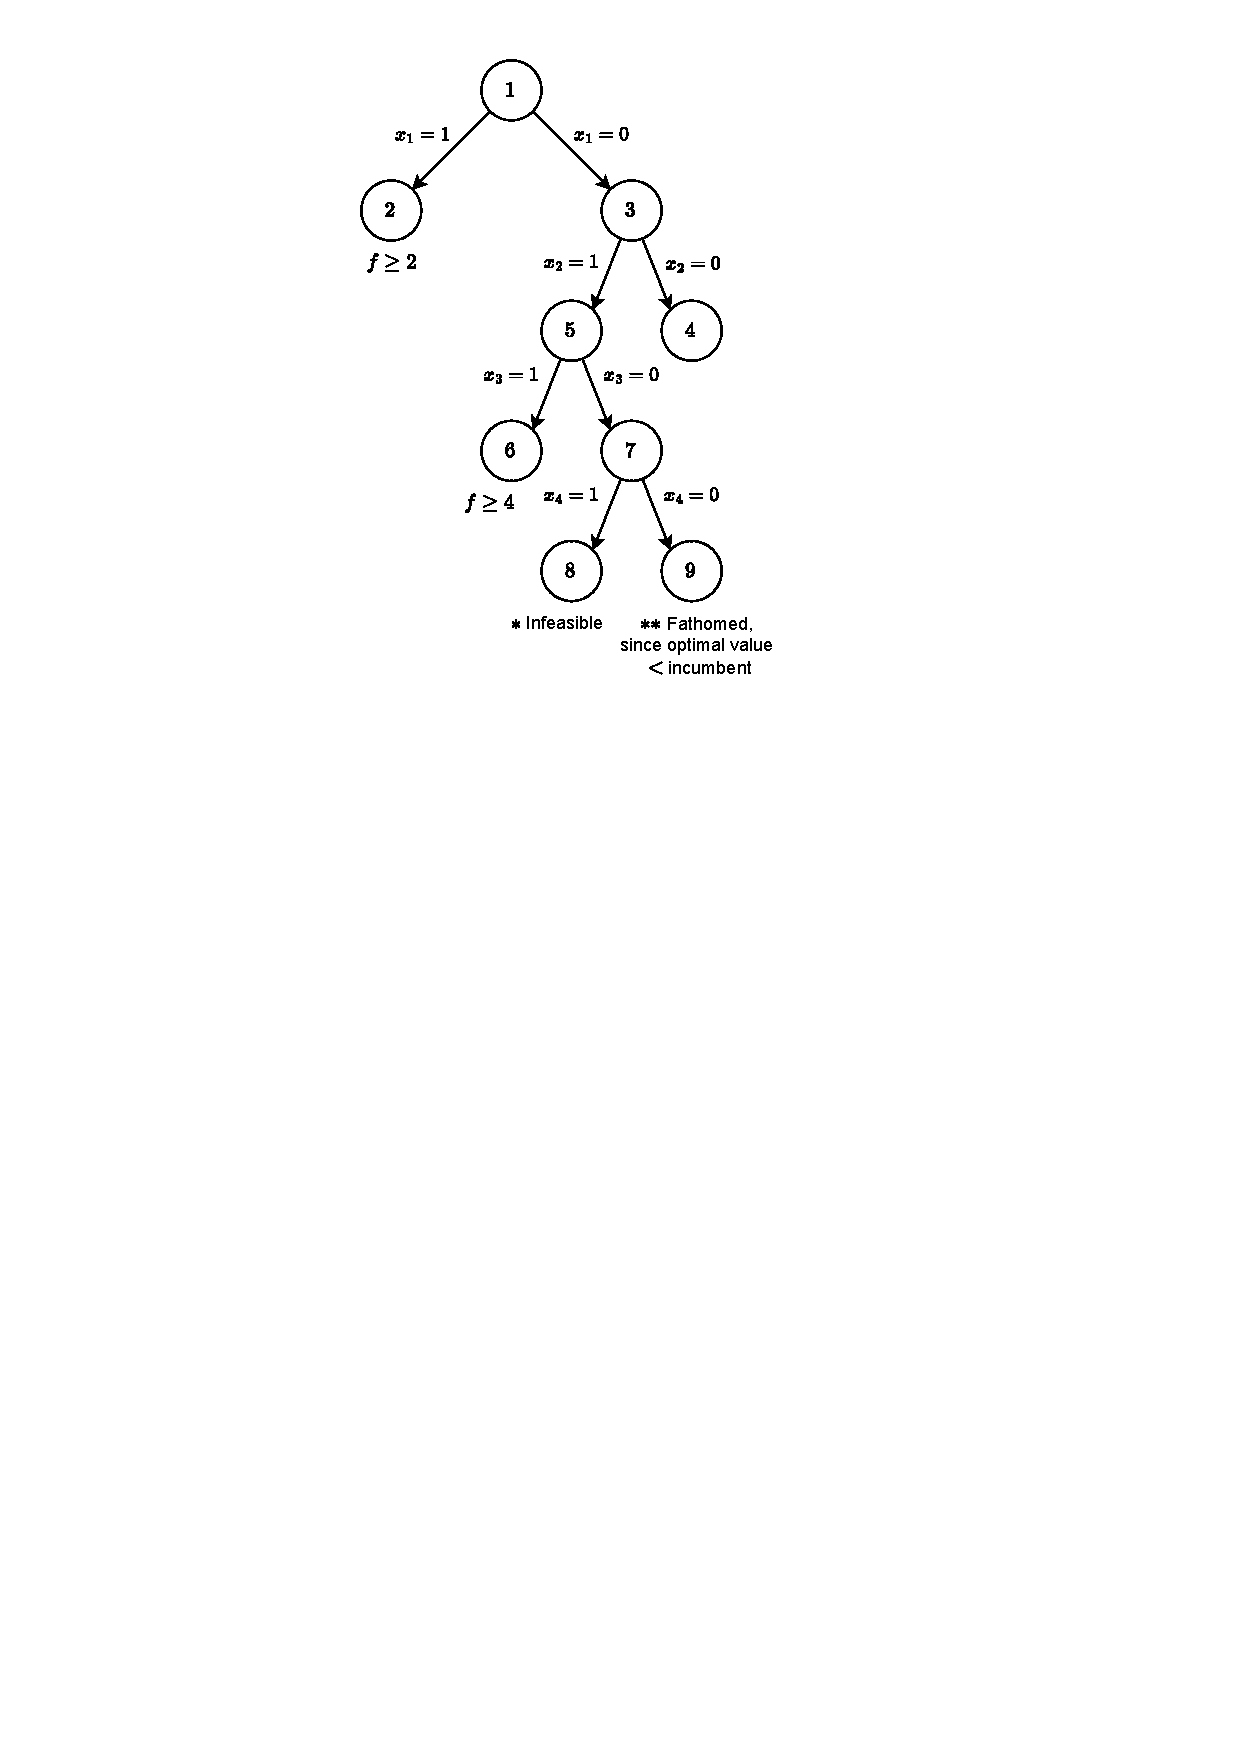
\includegraphics[width = 0.5\textwidth, trim = {6cm, 18cm, 6cm, 0cm}, clip]{document/operation_1.pdf}
\end{figure}

Note: If the coefficient of some $x_i$ in the objective function is positive, we may substitute $x^{\prime}_i= 1-x_i$.

\subsection{B. Cutting plane method}

Idea: Suppose that in the IP (\ref{1.29}), the LP relaxation (\ref{LP-3}) has an optimal solution $\bar{x}\notin\mathbb{Z}^n_{\ge 0}$. We add a new constraint into (\ref{LP-3}) which defines a hyberplane. The hyberplane ``cuts off'' $\bar{x}$ from the feasible set of (\ref{LP-3}) but none of the feasible integer points of (\ref{1.29}).

\begin{figure}[htbp]
    \centering
    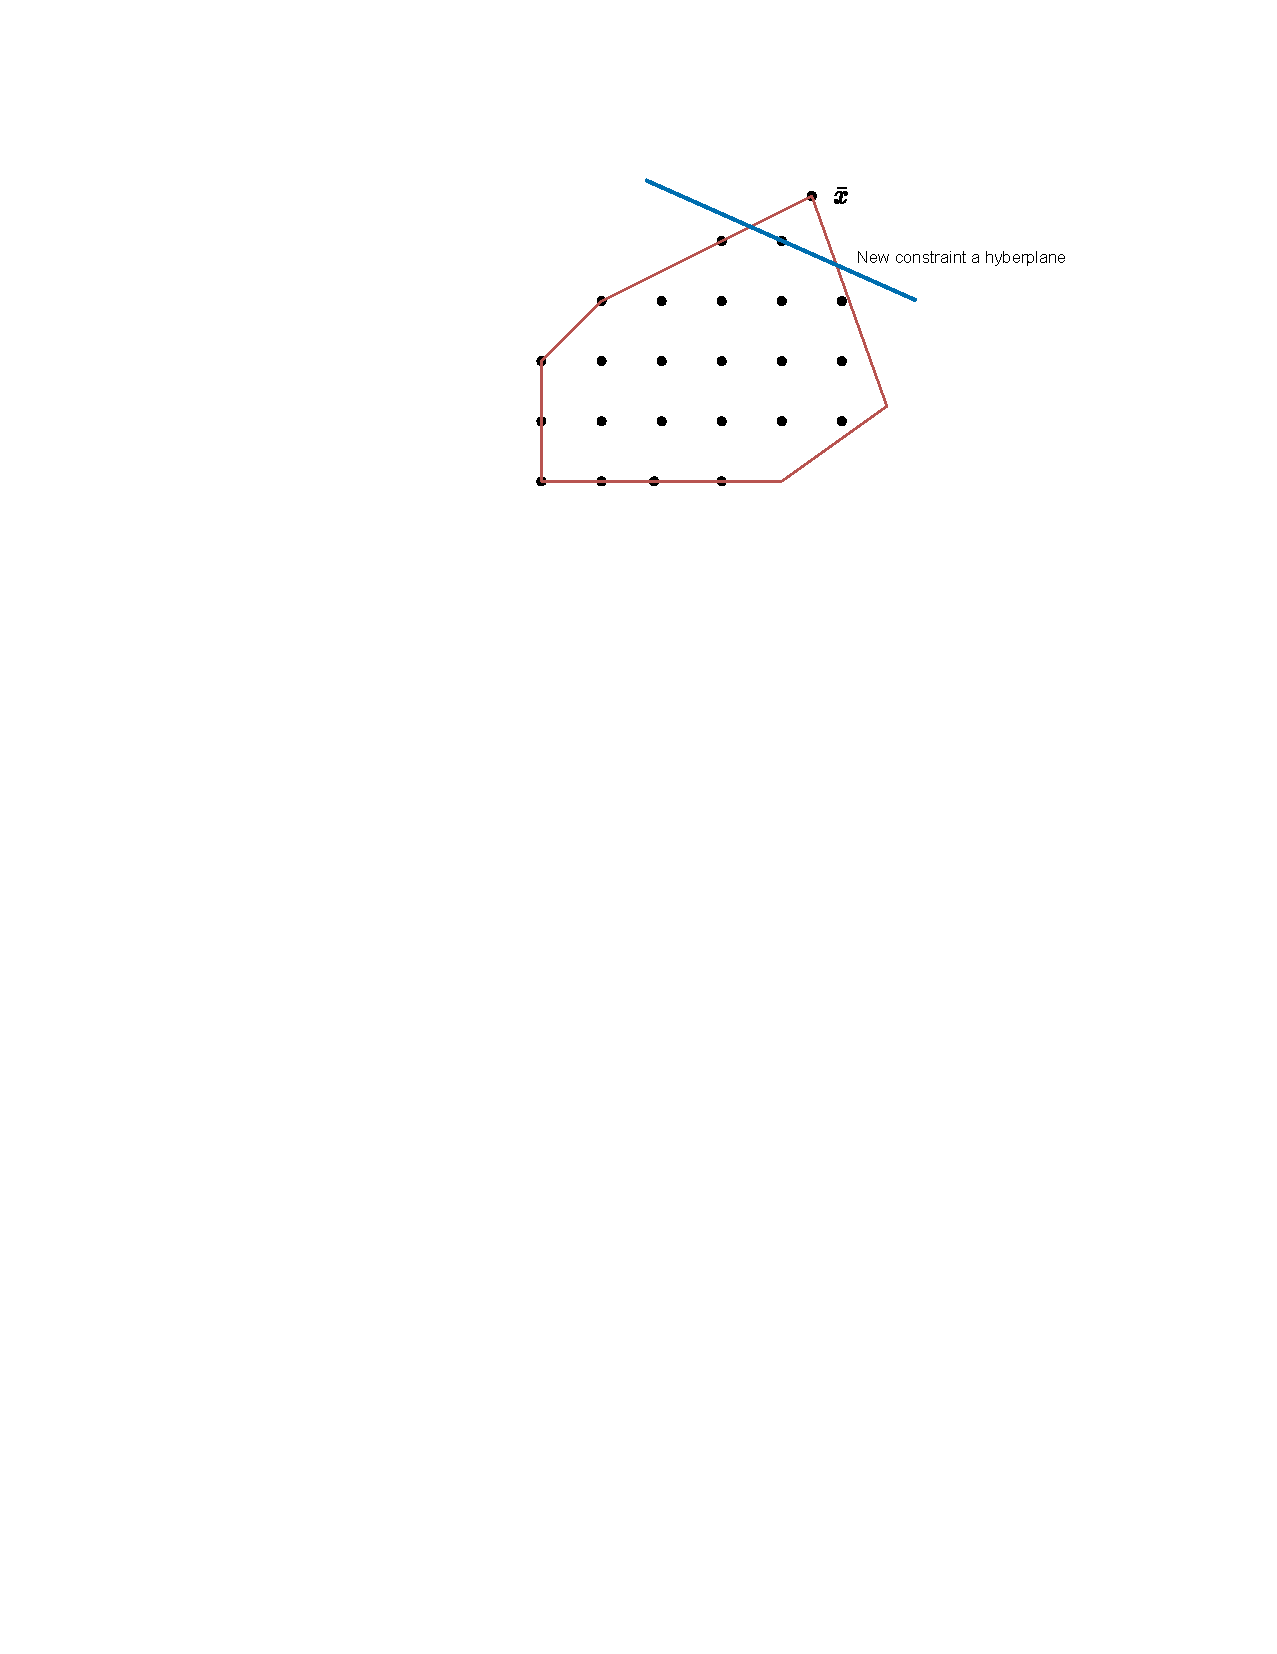
\includegraphics[width = 0.6\textwidth, trim = {6cm, 18cm, 0cm, 1cm}, clip]{document/2.drawio.pdf}
\end{figure}

We solve the new LP, and repeat the procedure until we find an optimal solution in $\mathbb{Z}_{\geqslant 0}^n$ for some LP.

Here, we assume the entries of $A, b, c$ in (\ref{1.29}) are in $\mathbb{Z}$, or equivalently, in $\mathbb{Q}$ (since we may clear fractions by multiplying by a suitable integer).

\begin{lemma}
    Lemma 1.19 Let $x_i\in\mathbb{Z}_{\ge 0}$, $a_i\in\mathbb{R}$ for $1\leqslant i\leqslant n$, and $b\in \mathbb{R}$. If $a_1x_1+a_2x_2+\cdots +a_nx_n=b$, then
    \begin{align*}
        &\left\lfloor a_1\right\rfloor x_1+\cdots+\left\lfloor a_n\right\rfloor x_n \leqslant\lfloor b\rfloor \text {, }\\
        \text{and}\quad & \left(a_1-\left\lfloor a_1\right\rfloor\right) x_1+\cdots+\left(a_n-\left\lfloor a_n\right\rfloor\right) x_n \geqslant b-\lfloor b\rfloor.
    \end{align*}
\end{lemma}

\begin{proof}
    We have
\begin{align*}
\begin{aligned}
b & =\left(a_1-\left\lfloor a_1\right\rfloor\right) x_1+\cdots+\left(a_n-\left\lfloor a_n\right\rfloor\right) x_n+\left\lfloor a_1\right\rfloor x_1+\cdots+\left\lfloor a_n\right\rfloor x_n \\
& \geqslant\left\lfloor a_1\right\rfloor x_1+\cdots+\left\lfloor a_n\right\rfloor x_n .
\end{aligned}
\end{align*}

Since $\left\lfloor a_1\right\rfloor x_1+\cdots+\left\lfloor a_n\right\rfloor x_n \in \mathbb{Z}$, we have $\left\lfloor a_1\right\rfloor x_1+\cdots+\left\lfloor a_n\right\rfloor x_n \leqslant\lfloor b\rfloor$.

Multiplying by $-1$, and adding $a_1x_1+a_2x_2+\cdots+a_nx_n =b$ gives $(a_1-\left\lfloor a_1\right\rfloor x_1 +\cdot + (a_n-\left\lfloor a_n\right\rfloor x_n \geqslant b_n-\left\lfloor b\right\rfloor$
\end{proof}

\begin{example}
    Use the cutting plane method to solve
    \begin{align}
        \max &\quad f=2x_1+3x_2 \label{1.33}
        \\
        & \left\lbrace\begin{array}{ll}
            -2x_1+2x_2&\leqslant 3  \\
            x_1+2x_2 &\leqslant 6\\
            4x_1 +5x_2&\leqslant 20\\
            x_1, x_2&\in\mathbb{Z}_{\geqslant 0}
        \end{array} \right.\nonumber
    \end{align}
\end{example}

Introduce slack variables $s_1, s_2, s_3\geqslant 0$ to the LP relaxation of (\ref{1.33}). By simplex method, we have
\begin{table}[H]
    \centering
    \begin{tabular}{cccccc|c}
         $x_1$ & $x_2$ & $s_1$ & $s_2$ & $s_3$ & $f$ & \\ \hline
         -2 & 2 & 1 & 0 & 0 & 0 & 3\\ 
         1 & 2 & 0 & 1& 0 & 0 & 6\\
         4 & 5 & 0 & 0 & 1 & 0 & 20\\ \hline
         -2 & -3 & 0 & 0 & 0 & 1 & 0
    \end{tabular}
\end{table}
After some work, we have
\begin{table}[H]
    \centering
    \begin{tabular}{cccccc|c}
         $x_1$ & $x_2$ & $s_1$ & $s_2$ & $s_3$ & $f$ &   \\
         0 & 1 & 0 & $\frac{4}{3}$ & $-\frac{1}{3}$ & 0 & $\frac{4}{3}$\\ \hline
         1 & 0 & 0 & $-\frac{5}{3}$ & $\frac{3}{2}$ & 0 & $\frac{10}{3}$\\
         0 & 0 & 1 & -6 & 2 & 0 & 7\\ \hline
         0 & 0 & 0 & $\frac{2}{3}$ & $\frac{1}{3}$ & 1 & $\frac{32}{3}$
    \end{tabular}
\end{table}

The final table says that we have not found an integer solution to the LP relaxation. The entries on the right of rows 1, 2, 4 are non-integers. Note that $f\in\mathbb{Z}_{\geqslant 0}$. We have
\begin{align*}
    \begin{array}{llll}
         x_2+\frac{4}{3}s_2-\frac{1}{3}s_3 = \frac{4}{3} & & \frac{1}{3}s_2 + \frac{2}{3}s_3\geqslant \frac{1}{3} & (1)  \\
         x_1 - \frac{5}{3}s_2 + \frac{2}{3}s_2 = \frac{10}{3} & \underset{\text{Lemma 1.19}}{\Longrightarrow} & \frac{1}{3}s_2 + \frac{2}{3}s_3\geqslant \frac{1}{3} & (2) \\
         \frac{2}{3}s_2 + \frac{1}{3}s_3 + f = \frac{32}{3} & & \frac{2}{3}s_2 + \frac{1}{3}s_3\geqslant \frac{2}{3} & (3)
    \end{array}
\end{align*}

Each of (1), (2), (3) is a \uline{Gomory fractional cut}. We see that (1) and(2) are the same. Note that (3)$\Longrightarrow$ (1), (2), since (3) $\Longrightarrow$ $\frac{1}{3}s_2+ \frac{1}{6}s_3\geqslant \frac{1}{3}$, which $\Longrightarrow$ (1), (2). Now
\begin{align*}
    (3) \Longleftrightarrow \frac{2}{3}(6-x_1-2x_2)+\frac{1}{3}(20-4x_1-5x_2)\geqslant \frac{2}{3} \Longleftrightarrow 2x_1+3x_2\leqslant 10
\end{align*}

Now we solve a new LP by adding the constraint (3), which we write as $-\frac{2}{3}s_2-\frac{1}{3}s_3+s_4=-\frac{2}{3}$ for a slack variable $s_3\geqslant 0$. We use the dual simplex method:
\begin{table}[H]
    \centering
    \begin{tabular}{c|cccccc|c}
            & $x_1$ & $x_2$ & $s_1$ & $s_2$ & $s_3$ & $s_4$ & \\ \hline
            $x_2$ & 0 & 1 & 0 & $\frac{4}{3}$ & $-\frac{1}{3}$ & 0 & $\frac{4}{3}$\\
            $x_1$ & 1 & 0 & 0 & $-\frac{5}{3}$ & $\frac{2}{3}$ & 0 & $\frac{10}{3}$ \\
            $s_1$ & 0 & 0 & 1 & -6 & 2 & 0 & -7\\
            $s_4$ & 0 & 0 & 0 & $-\frac{2}{3}$ & $-\frac{1}{3}$(pivot) & 1 & $-\frac{2}{3}$ \\ \hline
            $-f$ & 0 & 0 & 0 & $-\frac{2}{3}$ & $-\frac{1}{3}$ & 0 & $-\frac{32}{3}$
    \end{tabular}
\end{table}

Then we have:
\begin{table}[H]
    \centering
    \begin{tabular}{c|cccccc|c}
            & $x_1$ & $x_2$ & $s_1$ & $s_2$ & $s_3$ & $s_4$ & \\ \hline
            $x_2$ & 0 & 1 & 0 & 2 & 0 & -1 & 2\\
            $x_1$ & 1 & 0 & 0 & -3 & 0 & 2 & 2 \\
            $s_1$ & 0 & 0 & 1 & -10 & 0 & 6 & 3\\
            $s_3$ & 0 & 0 & 0 & 2 & 1 & -3 & 2 \\ \hline
            $-f$ & 0 & 0 & 0 & 0 & 0 & -1 & -10
    \end{tabular}
\end{table}

We find the integer optimal solution $(x_1, x_2) = (2, 2)$ for (\ref{1.33}). The optimal values is $f=10$.
\begin{remark}
    (1), (2) $\Longrightarrow$ $3x_1+4x_2\leqslant 15$, which gives a weaker cutting line that $2x_1+3x_2\leqslant 10$ from (3). In general, we may obtain several cutting planes in dimension $n$ which are incomparable.
    
    If we did not find an integer optimal solution, we may repeat the whole procedure.
\end{remark}

\section{Dynamic Programming}
\uline{\textcolor{MarkerColour}{\textsc{A dynamic programming (DP) problem}}} can be described as a problem that can be solved by solving a sequence of subproblems. DPs occur in many areas of OR, not just in optimisation theory. We consider some important example.
\subsection{A. Knapsack Problem}
We would like to prepare a knapsack of items, such as water bottles, apples, etc, for a camping trip. There are $n$ types of items, and each item of type $i$ has weight $a_i$ and a value of importance, or \uline{profit} $c_i (1\leqslant i\leqslant n)$. The knapsack can hold a total weight of b.

Thus we want to solve the DP
\begin{align}
    \max &\quad c^T x \nonumber \\
    &\left\lbrace\begin{array}{ll}
         a^Tx&\leqslant b  \\
         x&\in\mathbb{Z}_{\geqslant 0}^n
    \end{array}\right. \label{1.34}
\end{align}
where $c, a\in\mathbb{R}^n_{\geqslant 0}$, $b\in\mathbb{R}$. We have $x_i$ is the number of items of type $i$.

We may solve (\ref{1.34}) with a recurrence relation, as follows. For $a\leqslant d\leqslant b$, $1\leqslant k\leqslant n$. Let $S_k(d) =$ maximum profits that can be achieved by item types $k, k+1, \cdots, n$, if the knapsack has remaining weight $d$. We want $S_1(b)$.

Suppose we have assigned that values for $x_1, \cdots, x_{k-1}$. We want to assign a value for $x_k$, and the knapsack has remaining weight $d$. Then we require $0\leqslant x_k\leqslant \lfloor \frac{d}{a_k}\rfloor$. Adding the type $k$ items increases the profit by $c_kx_k$ and decreases the remaining weight $a_kx_k$. The best ``future contribution'' to the total profit in the knapsack is $S_{k+1}(d-a_kx_k)$. Thus 
\begin{align}
    S_k(d) = \max\{ c_k x_k + S_{k+1}(d-a_kx_k):\ 0\leqslant x_k\leqslant \lfloor\frac{d}{a_k}\rfloor\}, \ 1\leqslant k\leqslant n-1 \label{1.35}
\end{align}

\begin{example}
    Solve the IP
    \begin{align*}
        \max &\quad 4x_1 + 5x_2 + 6x_3\\
        & \left\lbrace\begin{array}{ll}
            3x_1+4x_2+5x_3&\leqslant 10 \\
            x_1,\ x_2,\ x_3 &\in\mathbb{Z}_{\geqslant 0}
        \end{array} \right.
    \end{align*}
\end{example}
\begin{solution}
    \uline{Stage 3} \ Find $S_3(d)$ for $0\leqslant d\leqslant 10$.
    \begin{align*}
        S_3(d) = \left\lbrace\begin{array}{lll}
            0, & \ 0\leqslant d<5, & \ (x_3 = 0)\\
            6, & \ 5\leqslant d<10, & \ (x_3 = 1)\\
            12, & \ d = 10, & \ (x_3 = 2)
        \end{array} \right.
    \end{align*}

    \uline{Stage 2} \ Find $S_2(d)$ for $0\leqslant d\leqslant 10$. (\ref{1.35}) $\Rightarrow$
    \begin{align*}
        S_2(d) = \max\{5x_2 + S_3(d -4x_2): 0\leqslant x_2\leqslant \lfloor\frac{d}{4}\lfloor\}. 
    \end{align*}
    
    $0\leqslant d<4$: $x_2 = 0$, $S_2(d) = S_3(d) = 0$.

    $4\leqslant d<8$: $x_2\in\{0, 1\}$, $S_2(d) = \max(S_3(d), 5+S_3(d-4)) = \max(S_3(d), 5) = \left\lbrace\begin{array}{ll}
        5, & \ 4\leqslant d<5  \\
        6, & \ 5\leqslant d<8
    \end{array} \right.$

    $8\leqslant d<10$: $x_2\in\{0, 1, 2\}$, 
    \begin{align*}
        S_2(d) = \max(S_3(d), 5+S_3(d-4), 10+S_3(d-8)) = \left\lbrace\begin{array}{ll}
        \max(6, 5, 10) = 10, & \ 8\leqslant d<9, \\
        \max(6, 11, 10) = 11, & \ 9\leqslant d< 10, \\
        \max(12, 11, 10) = 12, & \ d=10.
    \end{array} \right.
    \end{align*}

    \uline{Stage 1} \ Find $S_1(10)$. (\ref{1.35})$\Rightarrow$
    \begin{align*}
        S_1(10) &= \max\{4x_1, S_2(10-3x_1):\ 0\leqslant x_1\leqslant \lfloor\frac{10}{3}\rfloor\} \\
        & = \max\{S_2(10), 4 + S_2(7), 8 + S_2(4), 12 + S_2(1)\} \\
        & = \max\{12, 4+6, \boxed{8+5}, 12+0\} \\
        & = 13.
    \end{align*}

    $\mathrm{Optimal\ value} = 13$. Optimal solution: $x_1 = 2$.
    \begin{align*}
        S_2(4) = \max\{0, \boxed{5}\} = 5 \Rightarrow \ x_2=1\\
        x_3 = 0 \ \text{from} \ 4x_1+5x_2+6x_3 = 13
    \end{align*}
\end{solution}

We may more conveniently use a \uline{table method}, which is a common approach in DP problems. The values of $S_1(d)\ (0\leqslant d\leqslant 10)$ are also found.

\tikzset{>=stealth}

\begin{table}[H]
    \centering
    \begin{tabular}{|c|ccccccccccc|}
        \hline
        \diagbox{k}{d} & 0 & 1 & 2 & 3 & 4 & 5 & 6 & 7 & 8 & 9 & 10 \\ \hline
        3 & \uline{\color{red}{0}}${}^{\color{red}+5}$ & 0 & 0 & 0 & 0 & 6 & 6 & 6 & 6 & 6 & 12 \\ 
        2 & 0 & 0 & 0 & 0 & \uline{\color{red}{5}}${}^{\color{red}+8}$ & 6 & 6 & 6 & 10 & \uline{\color{blue}{11}} & 12 \\
        1 & 0 & 0 & 0 & 4 & 5 & 6 & 8 & 9 & 10 & 12 & \uline{\color{red}{13}}  \\ \hline
    \end{tabular}
    \caption{Example}
    \label{tab:example}
\end{table}

Again, maximum$=S_1(10) = 13$. To calculate the values of the $x_1$ achieving this maximum, we backtrack. See the entries in red. Note that if there is q tie during the back tracking, we may consider all possibilities to obtain all optimal solutions.

\uline{Table Method}
1. Fill in the first row $(k=n):\ S_n(d) = c_n\lfloor\frac{d}{a_n}\rfloor$.

2. Fill in each successive row $(n>k\geqslant 1)$ by using (\ref{1.35}). Note that each row depends only on the entries in the row above.

We may add more constraints to problem (\ref{1.34}). For two constraints, we have the ID:
\begin{align}
    \max &\quad c^T x \nonumber\\
    &\left\lbrace\begin{array}{l}
        a^Tx\leqslant b \\
        p^Tx\leqslant q\\
        x\in \mathbb{Z}^n_{\geqslant 0}
    \end{array} \right.\label{1.36}
\end{align}
where $c, a, q\in\mathbb{R}^n_{\geqslant 0}$, $b, q\in\mathbb{R}_{\geqslant 0}$.

We may interpret the second constraint as: Each item of type $i\ (1\leqslant i\leqslant n)$ has volume $p_i$, and the knapsack can also hold a maximum volume of $q$.

For $0\leqslant d\leqslant b$, $0\leqslant r\leqslant q$, $1\leqslant k\leqslant n$, let $S_k(d, r)$ be the maximum profit from item types $k, k+1, \cdots, n$ with remaining weight $d$ and volume $r$. We want $S_1(b, q)$. We may similarly obtain the following recurrence relation for (\ref{1.36})
\begin{align}
    S_k(d, r) = \max\{c_kx_k + S_{k-1}(d-a_kx_k, r-p_kx_k):\ 0\leqslant x_k\leqslant \min\left( \lfloor\frac{d}{a}_k\rfloor, \lfloor\frac{r}{p_k}\rfloor\right), \ 1\leqslant k\leqslant n-1\label{1.37}
\end{align}

\begin{example}
    Solve the IP
    \begin{align}
        \max & \quad 2x_1+3x_2 \nonumber \\
        & \left\lbrace\begin{array}{l}
            3x_1+4x_2\leqslant 12   \\
            x_1+5x_2\leqslant 10\\
            x_1, x_2\in\mathbb{Z}_{\geqslant 0}
        \end{array} \right.
    \end{align}
\end{example}
\begin{solution}
    \uline{Stage 2}\ For $0\leqslant d\leqslant 12$, $0\leqslant r\leqslant 10$, 
    \begin{align*}
        S_2(d, r) = \left\lbrace\begin{array}{ll}
            0, & \text{if} \ {\color{red}(d, r) \in\left([0, 12]\times[0, 10]\right) \backslash \left([4, 12]\times[5, 10]\right)}  \\
            3, &\text{if} \ {\color{blue}(d, r) \in \left([4, 12]\times[5, 10] \right)\backslash\left([8, 12]\times\{10\} \right)} \\
            6, &\text{if} \ {\color{gray}(d, r) \in [9, 12]\times \{10\}}
        \end{array} \right.
    \end{align*}

    \uline{Stage 1} \ (\ref{1.37}) $\Rightarrow$
    \begin{align*}
        S_1(12, 10) &= \max\{2x_1+S_2(12-3x_1, 10-x_1):\ 0\leqslant x_1\leqslant \min\left(\lfloor\frac{12}{3}\rfloor, \lfloor\frac{10}{1}\rfloor\right) = 4\} \\
        & = \max\{ S_2(12, 10), 2+S_2(9, 9), 4+S_2(6, 8), 6+S_2(3, 7), 8+S_2(0, 6) \}\\
        & = \max(6, 2+3, 4+3, 6+0, 8+0) \\
        & = 8
    \end{align*}

   Optimal value $ = 8$

   Optimal solution: $x_1 = 4, x_2 = 0$ for $2_x1+3x_2 = 8$.

   We may also use a table method by considering $k=2$ and computing $d$ versus $r$, then repeat for $k=1$.
\end{solution}

\subsection{B. 0-1 knapsack Problem}
We have $n$ items available, where item $i$ has weight $a_i$ and profit $c_i\ (1\leqslant i\leqslant n)$. We want to place some of the items into a knapsack which holds a maximum weight $b$, and maximise the profit. We have the version of the knapsack problem where repetitions of the items are not allowed, {\color{red}\uline{or the 0-1 knapsack problem}} (a BIP).
\begin{equation}
    \begin{aligned}
        \max & \quad c^T x\\
        &\left\lbrace\begin{array}{ll}
            a^Tx\leqslant b  &\\
            x_i\in\{0, 1\} & 1\leqslant i\leqslant n
        \end{array} \right.
    \end{aligned}
    \label{1.38}
\end{equation}
where $c, a\in\mathbb{R}^n_{\geqslant 0}$, $b\in\mathbb{R}_{\geqslant 0}$. The recurrence relation for (\ref{1.38}) is slightly different. For $0\leqslant d\leqslant b$, $1\leqslant k\leqslant n$, let $S_k(d)$ be the maximum profit from items $k, k+1, \cdots, n$ if the knapsack has remaining weight $d$.

Similar to (\ref{1.35}), we have, for $1\leqslant k\leqslant n-1$, 
\begin{align}
    S_k(d) = \left\lbrace\begin{array}{ll}
        S_{k+1}(d),  & \ \textrm{if } 0\leqslant d<a_k \\
        \max(S_{k+1}(d), c_k+S_{k+1}(d-a_k)), &\ \textrm{if } a_k\leqslant d\leqslant b
    \end{array}\right. \label{1.39}
\end{align}

\begin{example}
    Solve the BIP 
    \begin{align*}
        \max &\quad 8x_1 + 11x_2 + 6x_3 + 4x_4 \\
        & \left\lbrace\begin{array}{ll}
            5x_1 + 7x_2 + 4x_3 + 3x_4 &\leqslant 14 \\
            x_i \in\{0, 1\}, & 1\leqslant i\leqslant 4
        \end{array} \right.
    \end{align*}
\end{example}

\uline{\textsc{\textcolor{MarkerColour}{Stage 4}}}
\begin{align*}
    S_4(d) = \left\lbrace\begin{array}{lll}
        0, & \text{if } 0\leqslant d < 3 & (x_4=0)  \\
        \boxed{4}, & \text{if } 3\leqslant d\leqslant 14 & (x_4=1) 
    \end{array} \right.
\end{align*}

\uline{\textsc{\textcolor{MarkerColour}{Stage 3}}}
\begin{align*}
    &(\ref{1.39}) \Longrightarrow \\
    & S_3(d) = S_4(d) = \left\lbrace\begin{array}{lll}
        0, & \text{if } 0\leqslant d < 3 & (x_4=0)  \\
        4, & \text{if } 3\leqslant d\leqslant 4 & (x_4=1) 
    \end{array} \right. \\
    & S_3(d) =\max(S_4(d), \boxed{6+S_4(d-4)})\\
    & = \left\lbrace\begin{array}{ll}
             \max(4, 6+0) = 6, & \text{if } 4\leqslant d<7  \\
             \max(4, \boxed{6+4}) = 10, & \text{if } 7\leqslant d\leqslant 14
    \end{array} \right.
\end{align*}

\uline{\textsc{\textcolor{MarkerColour}{Stage 2}}}
\begin{align*}
    S_2(d) &= S_3(d) = \left\lbrace\begin{array}{ll}
        0, & \text{if } 0\leqslant d< 3\\
        4, &\text{if } 3\leqslant d<4\\
        6, &\text{if } 4\leqslant d < 7
    \end{array} \right. \\
    S_2(d) &= \max(S_3(d), \boxed{11+S_3(d-7)}) \\
    & = \left\lbrace\begin{array}{ll}
        \max(10, 11+0) = 11, & \text{if } 7\leqslant d<10 \\
        \max(10, 11+4) = 14, &\text{if } 10\leqslant d< 11\\
        \max(10, 11+6) = 17, &\text{if } 11\leqslant d\leqslant 14\\
        \max(10, \boxed{11+10}) = 21, &\text{if } d=14
    \end{array} \right.
\end{align*}

\uline{\textsc{\textcolor{MarkerColour}{Stage 1}}}
\begin{align*}
    (\ref{1.39}) \Longrightarrow S_1(14) = \max(\boxed{S_2(14)}, 8+S_2(14-5)) = \max(\boxed{21}, 8+11) = 21
\end{align*}

Optimal value $= 21$. Optimal solution: $(x_1, x_2, x_3, x_4) = (0, 1, 1, 1)$.

\uline{\textsc{\textcolor{MarkerColour}{Table Method}}}

\begin{table}[H]
    \centering
    \begin{tabular}{|c|ccccccccccccccc|c|}
        \hline
        \diagbox{k}{d} & 0 & 1 & 2 & 3 & 4 & 5 & 6 & 7 & 8 & 9 & 10 & 11 & 12 & 13 & 14 & \textcolor{red}{Optimal solution} \\ \hline
        4 & \boxed{0} & 0 & 0 & \boxed{4} & 4 & 4 & 4 & 4 & 4 & 4 & 4 & 4 & 4 & 4 & 4 & \textcolor{red}{$x_4 = 1$} \\
        3 & 0 & 0 & 0 & 4 & 6 & 6 & 6 & \boxed{10} & 10 & 10 & 10 & 10 & 10 & 10 & 10 & \textcolor{red}{$x_3 = 1$} \\
        2 & 0 & 0 & 0 & 4 & 6 & 6 & 6 & 11 & 11 & 11 & 15 & 17 & 17 & 17 & \boxed{21} & \textcolor{red}{$x_2 = 1$}\\
        1 & 0 & 0 & 0 & 4 & 6 & 8 & 8 & 11 & 12 & 14 & 15 & 17 & 19 & 19 & \boxed{21} & \textcolor{red}{$x_1 = 0$} \\ \hline
    \end{tabular}
    \caption{Table Method}
\end{table}

As before, we may generalise (\ref{1.38}) by having two or more constraints.

\subsection{C. Resource allocation problem}
Suppose we have a total budget (or resource) $b\in\mathbb{Z}_{\geqslant 0}$, to be spent on $n$ types of activities. If $x_i\in\mathbb{Z}_{\geqslant 0}$ units of activity type $i$ are performed, there is a profit of $f_i(x_i)$, where $f_i:\ \{0, 1, \cdots, b\}\to \mathbb{R}_{\geqslant 0}$ is a non-decreasing function with $f_i(0) = 0$, $\forall\ 1\leqslant i\leqslant n$. 

We want to solve the IP:
\begin{align}
    \max & \quad \sum\limits_{i=1}^n f_i(x_i) \nonumber \\
    & \left\lbrace\begin{array}{rl}
        \sum\limits_{i=1}^n x_i & = b  \\
        x & \in\mathbb{Z}^n_{\geqslant 0}
    \end{array} \right.\label{1.40}
\end{align}

For $0\leqslant d\leqslant b$, $1\leqslant k\leqslant n$, let $S_k(d)$ be the maximum profit from activities of type $k, k+1, \cdots, n$, with a budget of $d$ remaining. We want $S_1(b)$. Similarly, we have the following recurrence relation for (\ref{1.40}):
\begin{align}
    S_k(d) = \max\{f_k(x_k) + S_{k+1}(d - x_k):\ 0\leqslant x_k\leqslant d\}, \ 1\leqslant k\leqslant n-1  \label{1.41}
\end{align}

Note that $S_n(d) = f_n(d)$ for $d=1, 2, \cdots, b$, and $S_k(0) = 0$ for $k=1, 2, \cdots, n$.

\begin{example}
    Suppose 4 doctors are assigned to 3 hospitals. For $i = 1, 2, 3$ and $y = 1, 2, 3, 4$, let $f_i(y)$ be the number of patients that $y$ doctors can serve per hour in hospital $i$ given by the table
    \begin{table}[H]
        \centering
        \begin{tabular}{|c|ccc|}
            \hline
            $y =$ Number pf doctors & $f_1(y)$ & $f_2(y)$ & $f_3(y)$ \\ \hline
            0 & 0 & \boxed{0}& 0 \\
            1 & 4 & 2 & \boxed{5}\\
            2 & 6 & 4 & 7 \\
            3 & \boxed{9}& 7 & 8 \\
            4 & 10 & 11 & 9 \\
            \hline
        \end{tabular}
        \caption{number of patients that $y$ doctors can serve per hour}
        \label{tab:doctor}
    \end{table}
    What is the maximum umber of patients that can be served per hour, across 3 hospitals?
\end{example}

We have problem (\ref{1.40}) where $b=4$, and $x_1 =$ number of doctors assigned to hospital $i$. 

\uline{\textsc{\textcolor{MarkerColour}{Stage 3}}}
\begin{align*}
    S_3(d) = f_3(d), \ 0\leqslant d\leqslant 4
\end{align*}
\uline{\textsc{\textcolor{MarkerColour}{Stage 2}}}
\begin{align*}
    S_2(0) &= 0 \\
    (\ref{1.41}) \Longrightarrow S_2(d) &= \max \{f_2(x_2) + S_3(d-x_2): \ 0\leqslant x_2\leqslant d\} \\
    S_2(1)  & = \max\{\boxed{0+S_3(1)}, 2+f_3(0) \} = \max\{\boxed{5}, 2\} = 5 \\
    S_2(2) &= \max\{0+S_3(2), 2+S_3(1), 4+S_3(0)\} = \max\{7, 7, 4\} = 7 \\
    S_2(3) &= \max\{0+S_3(3), 2+S_3(2), 4+S_3(1), 7+S_3(0)\} = \{8, 9, 9, 7\} = 9 \\
    S_2(4) &= \max\{0+S_3(4), 2+S_3(3), 4+S_3(2), 7+S_3(1), 11+S_3(0)\} = \{9, 10, 11, 12, 11\} = 12
\end{align*}

\uline{\textsc{\textcolor{MarkerColour}{Stage 1}}}
\begin{align*}
    \text{(\ref{1.41})} = S_1(4) &= \max\{f_1(x_1)+S_2(4-x_1):\ 0\leqslant x_1\leqslant 4\} \\
    & = \max\{0+S_2(4), 4+S_2(3), 6+S_2(2), \boxed{9+S_2(1)}, 10+S_2(0)\} = \max\{12, 13, 13, \boxed{14}, 10\} = 14
\end{align*}

Optimal value $= 14$. Optimal solution $:(x_1, x_2, x_3) = (3, 0, 1)$. See the circled entries in the above table. 

\uline{\textsc{\textcolor{MarkerColour}{Table Method}}}
\begin{table}[H]
    \centering
    \begin{tabular}{|c|cccccc|}
        \hline
        \diagbox{k}{d} & 0 & 1 & 2 & 3 & 4 & \textcolor{red}{Optimal solution} \\ \hline
        3 & 0 & 5 & 7 & 8 & 9 & \textcolor{red}{$x_3 = 1$} \\
        2 & 0 & 5 & 7 & 9 & 12 & \textcolor{red}{$x_2 = 0$} \\
        1 & 0 & 5 & 9 & 11 & 14 & \textcolor{red}{$x_1 = 3$} \\ \hline
    \end{tabular}
    \caption{Table Method}
    \label{table method-2}
\end{table}

\chapter{Game Theory}
\section{Introduction}
Suppose two players Alice and Bob play a game. The set of choices, called \uline{\textsc{\textcolor{MarkerColour}{strategies}}}, available to Alice and Bob, are $S_1 = \{\alpha_1, \cdots, \alpha_m\}$ and $S_2 = \{\beta_1, \cdots, \beta_n\}$. If Alice and Bob choose $\alpha_i$ and $\beta_j$, then they win $a_{ij}$ and $b_{ij}$ respectively. The matrices $A, B\in\mathbb{R}^{m\times n}$ are the \uline{\textsc{\textcolor{MarkerColour}{Payoff Matrices}}} for Alice and Bob. 

What should each player do to try and maximise their winnings? 

\begin{example}[Rock-Scissors-Paper]
    We have $S_1 = S_2 = \{\text{Rock}, \text{Scissors}, \text{Paper}\}$. Rock beats scissors, scissors beats paper, paper beats rock, and the same choices is a tie. If there is a win, the loser pays the winner $\yen 1$. We may superimpose the payoff matrices as 
    \begin{table}[H]
        \centering
        \begin{tabular}{|c|ccc|}
                \hline
                \diagbox{Alice}{Bob} & $\beta_1 = \text{Rock}$ & $\beta_2 = \text{Scissors}$ & $\beta_3 = \text{Paper}$ \\ \hline
                $\alpha_1 = \text{Rock}$ & (0, 0) & (1, -1) & (-1, 1) \\
                $\alpha_2 = \text{Scissors}$ & (-1, 1) & (0, 0) & (1, -1) \\
                $\alpha_2 = \text{Paper}$ & (1, -1) & (-1, 1) & (0, 0) \\ \hline
        \end{tabular}
        \caption{Rock-Scissor-Paper}
        \label{2.1}
    \end{table}
    (\ref{2.1}) is also called the \uline{\textsc{\textcolor{MarkerColour}{Payoff Matrices}}}.
\end{example}

\begin{example}[Prisoner's Dilemma]
    Alice and Bob have been arrested and accused of jointly committing a robbery. The police have offered each of them to either remain silent, or testify the other suspect. 
    \begin{itemize}
        \item If they both remain silent, they are both jailed for 1 year.
        \item If they both testify, they are both jailed for 3 years.
        \item If one suspect testifies, and the other remains silent, then one who testifies is set free, while the other is jailed for 6 years.
    \end{itemize}
    Thus, $S_1 = S_2 = \{\text{Silent}, \text{Testify}\}$. They are then taken into separate rooms and questioned, so they are unaware of the other's action. 
\end{example}

The payoff matrix is
\begin{table}[H]
    \centering
    \begin{tabular}{|c|cc|}
        \hline
        \diagbox{Alice}{Bob}  &  $\beta_1 = $ Silent & $\beta_2 = $ Testify\\ \hline
        $\alpha_1 = $ Silent  & (-1, -1) & (-6, 0) \\
        $\alpha_2 = $ Testify & (0, -6) & (-3, 3) \\ \hline
    \end{tabular}
    \caption{The payoff matrix}
    \label{tab:example-2}
\end{table}

In games such as Examples 1 and 2, the following may be assumed:
\begin{itemize}
    \item[$\bullet$] The games are \uline{full information}: Both Alice and Bob know that the other player knows both strategy sets $S_1, S_2$, and the payoff matrix.
    \item[$\bullet$] The games are \uline{``non-cooperative''}: Alice and Bob are not in an alliance, and each plays to promote only their own winnings.
    \item[$\bullet$] Alice and Bob both play \uline{``rationally''}. That is, if Alice chooses $\alpha_i$, then Bob should try to choose $\beta_j$ to promote his winnings, and vice versa.
\end{itemize}

We may also consider dropping any of these assumptions. Such games may be extended to more than two players. These games have applications in economics, political science (eg: voting), computer science, etc.

\section{Two-player zero-sum and constant-sum games}\label{section 2.2}
If in the game between Alice and Bob, we have $A+B=0$, then we have a \uline{zero-sum game}. Thus, Alice wins $a_{ij}$ $\Longrightarrow$ Bob loses $a_{ij}$, or Bob pays Alice $a_{ij}$. Example 1 is a zero-sum game.

It suffices to study only the matrix $A$. $A$ ``rational'' situation may occur as follows. If Alice chooses $\alpha_i$, she should expect Bob to choose $\beta_j$ to maximise his winnings (thus minimise Alice's winnings). So Alice can win $\geqslant \max\limits_{i}\min\limits_{j}a_{ij}$. Likewise, if Bob choose $\beta_j$, he should expect Alice to choose $\alpha_i$ to maximise her winnings and Bob's losses. So Bob can lose $\leqslant \min\limits_{j}\max\limits_{i} a_{ij}$.

If we have 
\begin{align}
    \max\limits_i \min\limits_j a_{ij} = \min\limits_j \max\limits_i a_{ij} = v,\ \text{says} \nonumber
\end{align}
then any entry of $A$ is the same row as $\max\limits_i \min\limits_j a_{ij}$, and same column as $\min\limits_j\max\limits_i a_{ij}$, is a \uline{saddle point}, or an \uline{equilibrium point}. In this case, we say the game has \uline{value} $v$.

Indeed, we have the following result.
\begin{theorem}\label{Th 2.1}
    Suppose we have a zero-sum game between Alice and Bob, where $A\in\mathbb{R}^{m\times n}$ is Alice's payoff matrix.

    (a) We have $\max\limits_i\min\limits_j a_{ij} \leqslant \min\limits_{j}\max\limits_{i} a_{ij}$.

    (b) An entry $a_{ij}\in A$ is a saddle point if and only if $a_{ij}$ is the smallest number is row $i$, and the largest number in column $j$.

    (c) Any two saddle points have the same value.
\end{theorem}
\begin{proof}
    HW3
\end{proof}

Thus, if the game has a saddle point with value $v$, then we have rational situation that Alice/Bob are guaranteed to win/lose $v$, if they choose $\alpha_i$ and $\beta_j$ corresponding to a saddle point. If Alice deviates to some $\alpha_k$, then Th \ref{Th 2.1} (b) $\Rightarrow$ her winnings can become $< v$. A similar situation applies to Bob if her deviates to some $\beta_l$.

\begin{example}
    Suppose we have the payoff matrix $A$: 
    \begin{table}[H]
        \centering
        \begin{tabular}{|c|cccc|c|}
            \hline
            \diagbox{Alice}{Bob} & $\beta_1$ & $\beta_2$ & $\beta_3$ & $\beta_4$ & \textcolor{red}{Row min} \\ \hline
            $\alpha_1$ & 3 & 4 & 10 & 5 & \textcolor{red}{3}\\
            $\alpha_2$ & 8 & 5 & $-2$ & 1 & \textcolor{red}{$-2$}\\
            $\alpha_3$ & 6 & \boxed{5} Saddle Point & 7 & 9 & \textcolor{red}{\boxed{5}$\leftarrow \max\limits_{i}\min\limits_{j}a_{ij}$} \\
                \textcolor{blue}{Column max}$\rightarrow$ & \textcolor{blue}{8} & \textcolor{blue}{\boxed{5}$\leftarrow \min\limits_j\max\limits_i a_{ij}$} & \textcolor{blue}{10} & \textcolor{blue}{9} & \\ \hline
        \end{tabular}
        \caption{Payoff Matrix}
        \label{example-3}
    \end{table}
\end{example}

We see that there is a saddle point with value $5$ as indicated. Note that there are other entries also with value $5$. If the game is played rationally, the Alice win $5$ units by choosing $\alpha_3$, and Bob loses $5$ units by choosing $\beta_2$.

Similarly, suppose we have the payoff matrices
\begin{align}
    A = \left(\begin{array}{cccc}
        8 & \boxed{\circled{4}} & 4 & \boxed{\circled{4}}  \\
        9 & 3 & 2 & \boxed{4}  \\
        5 & \boxed{\circled{4}} & 7 & \boxed{\circled{4}}  \\
        0 & \boxed{4} & 8 & 2  \\
    \end{array} \right) \quad \quad \quad A = \left(\begin{array}{ccc}
        0 & \boxed{1} & \circled{-1}  \\
        \circled{-1} & 0 & \boxed{1}  \\
        \boxed{1} & \circled{-1} & 0  \\
    \end{array} \right) \nonumber
\end{align}

The first matrix has four saddle points with value $4$. The second, which is from Example 1, has no saddle point.

Now suppose that $A+B=C$, where every entry of $C$ is the same, say equal to $c$. Then we have a \uline{constant-sum game}. A zero-sum game is thus a constant-sum game with $c=0$. Constant-sum games generalise zero-sum games, since Bob aims to maximise $b_{ij} = c-a_{ij}\Longleftrightarrow$ Bob aims to minimise $a_{ij}$. Then notions of rationality, and saddle points of $A$, remain valid. We also have Th \ref{Th 2.1} with ``constant-sum'' in place of ``zero-sum''.

Back to a zero-sum game, what happens if the matrix $A$ has no saddle point? If Alice and Bob still play rationally, then they would use \uline{mixed strategy}, where they make their choices according to some probability distributions. In the case where they choose $\alpha_i$ and $\beta_j$ with probability $1$, we have \uline{pure strategy}. Thus in particular, if $A$ has a saddle point, then we have pure strategy since Alice and Bob would always choose $\alpha_i$ and $\beta_j$ corresponding to a saddle point.

We have
\begin{table}[H]
    \centering
    \begin{tabular}{|c|ccc|}
        \hline
        \diagbox{Alice}{Bob} & $\beta_1$ & $\cdots$ & $\beta_n$ \\ \hline
        $\alpha_1$ & $a_{11}$ & $\cdots$ & $a_{1n}$ \\
        $\vdots$ & $\vdots$ & & $\vdots$ \\
        $\alpha_m$ & $a_{m1}$ & $\cdots$ & $a_{mn}$ \\ \hline
    \end{tabular}
\end{table}

For $1\leqslant 1\leqslant m$, suppose Alice choose $\alpha_i$ with probability $x_i\in [0, 1]$, so that $x_1 + \cdots + x_m = 1$. For example, $m=2$, $x_1 = x_2 = \frac{1}{2}$ means Alice throws a fair coin to make her decision. Then Alice's expected winnings, if Bob chooses $\beta_j\ (1\leqslant j\leqslant n)$, is $a_{1j}x_1 + \cdots + a_{mj}x_m$. So Alice is expected to win at least
\begin{align*}
    u = \min\{a_{1j}x_1 + \cdots + a_{mj}x_m: \ 1\leqslant j\leqslant n\}
\end{align*}

Thus, Alice wants to choose $x_1, x_2, \cdots, x_m$ s.t. $u$ is maximised. We have Alice's LP
\setcounter{equation}{2}
\begin{align}
    \max & \quad u \nonumber \\
    & \left\lbrace\begin{array}{cl}
        a_{11}x_1 + \cdots + a_{m1}x_m &\geqslant u  \\
        \vdots & \\
        a_{1n}x_1 + \cdots + a_{mn}x_m & \geqslant u \\
        x_1 + \cdots + x_m & = 1 \\
        x_i\geqslant 0 \ (1\leqslant i \leqslant m), & u\in\mathbb{R} 
    \end{array} \right.\label{2.3}
\end{align}

Writing $u=u_1-u_2$ where $u_1, u_2\geqslant 0$, we convert to the form of (\ref{LP standard}):
\begin{align}
    \max & \quad c^T \Tilde{x} \nonumber \\
    & \left\lbrace\begin{array}{cc}
       A\Tilde{x}  &\leqslant b  \\
         \Tilde{x}&\geqslant 0 
    \end{array} \right.\label{2.4}
\end{align}
where
\begin{align*}
    A = \left(\begin{array}{ccc}
        -A^T & \mathbbm{1}_n & -\mathbbm{1}_n \\
        \mathbbm{1}_m^T & 0 & 0 \\
        -\mathbbm{1}_m^T & 0 & 0
    \end{array} \right)\in\mathbb{R}^{(n+2)\times(m+2)},\quad b = \left(\begin{array}{c}
         0  \\
         \vdots \\
         0 \\
         1 \\
         -1 
    \end{array} \right) \in\mathbb{R}^{n+2}, \quad c = \left(\begin{array}{c}
         0  \\
         \vdots \\
         0 \\
         1 \\
         -1 
    \end{array} \right) \in\mathbb{R}^{m+2} \\
    \Tilde{x} = \left(\begin{array}{c}
         x_1  \\
         \vdots \\
         x_m \\
         u_1 \\
         u_2 
    \end{array} \right) \in\mathbb{R}^{m+2}, \quad \text{and} \quad \mathbbm{1}_k = \underbrace{(1\ \cdots \ 1)}\limits_{k}^T
\end{align*}

Similarly, for $1\leqslant i\leqslant n$, suppose Bob choose $\beta_j$ with probability $y_j\in[0, 1]$, so that $y_1+\cdots + y_n = 1$. Then Bob's expected loss, if Alice chooses $\alpha_i\ (1\leqslant i\leqslant m)$, is $a_{i1}y_1 + \cdots + a_{in}y_n$. So Bob is expected to lose at most
\begin{align*}
    w = \max\{a_{i1}y_1 + \cdots + a_{in}y_n:\ 1\leqslant i\leqslant m\}
\end{align*}

Thus, Bob wants to choose $y_1, \cdots, y_n$ s.t. $w$ is minimised. We have Bob's LP:
\begin{align}
    \min & \quad w \nonumber \\
    & \left\lbrace\begin{array}{cl}
        a_{11}y_1 + \cdots + a_{1n}y_n &\leqslant w  \\
        \cdots & \\
        a_{m1}y_1 + \cdots + a_{mn}y_n &\leqslant w \\
        y_1 + \cdots y_n & = 1 \\
        y_j\geqslant 0\ (1\leqslant j\leqslant n), & w\in \mathbb{R} 
    \end{array} \right.\label{2.5}
\end{align}

Writing $w=w_1-w_2$, where $w_1, w_2\geqslant 0$, we convert to the form of (\ref{dual LP}):
\begin{align}
    \min & \quad b^T\Tilde{y} \nonumber \\
    & \left\lbrace\begin{array}{ll}
        \Tilde{A}^T\Tilde{y} & \succeq c  \\
        \Tilde{y} &\succeq 0
    \end{array} \right. \label{2.6}
\end{align}
where $\Tilde{y} = \left( y_1\ \cdots \ y_n \ w_1 \ w_2\right)^T\in\mathbb{R}^{n+2}$.

Now clearly (\ref{2.4}) and (\ref{2.6}) are dual LPs. It is easy to show that both (\ref{2.4}) and (\ref{2.6}) are feasible and bounded. By Th 1.7, we have strong duality. Let both optimal values of (\ref{2.4}) and (\ref{2.6}) be $v$. We say that $v$ is the \uline{value} of the game.

We have the following important result in game theory. 
\begin{theorem}(Von Neumann Minimax Theorem)
    Suppose that Alice and Bob play a zero-sum game rationally, using mixed strategy. Let $A\in\mathbb{R}^{m\times n}$ be Alice's payoff matrix. Then $\exists$ optimal probability distributions $\bar{x} = \left( x_1, \cdots, x_m\right)$ and $\bar{y} = \left( y_1, \cdots, y_n\right)$ for Alice and Bob, s.t. Alice is expected to win $\geqslant v$, and Bob is expected to lose $\leqslant v$, where $v$ is the value of the game.

    Moreover,
    \begin{align}
        \max\limits_x \min\limits_y x^T A y = \min\limits_y \max\limits_x x^T A y = v \label{2.7}
    \end{align}
    where the max and min are taken over $x\in \left[0, 1\right]^m$, $y\in\left[0, 1\right]^n$ with $\sum\limits_{i=1}^m x_i = \sum\limits_{j=1}^n y_j = 1$. Also, $\bar{x}$ and $e_j\i\mathbb{R}^n$ attain $\max\limits_x \min\limits_y x^Ay = v$ for some $j$, and $e_i\in\mathbb{R}^m$ and $\bar{y}$ attain $\min\limits_y \max\limits_x x^TAy = v$ from some $i$. (\uline{\textbf{Recall:}} $e_i\in\mathbb{R}^k$ is the standard basis vector, $e_i = \overbrace{\left(0 \ \cdots \ 1 \ 0 \ \cdots \ 0 \right)^T}\limits^{k}$).
\end{theorem}
\begin{proof}
    From the above discussion, it suffices to prove (\ref{2.7}). Note that the set of $y\in[0,1]^n$ with $\sum\limits_{j=1}^n y_j = 1$ defines a simplex in $\mathbb{R}^n$, whose extreme points are $e_1, \cdots, e_n$. For any fixed $x$, since $x^TAy$ is a linear function in $y$, we have $\min\limits_y x^TAy = \min\limits_j x^TAe_j$ by Th 1.2. Thus, 
    \begin{align*}
        \max\limits_x \min\limits_y x^TAy = \max\limits_x \min\limits_j x^TAe_j  \underset{\text{(2.3), Th 1.7}}{=} v.
    \end{align*}

    Similarly, 
    \begin{align*}
        \min\limits_y \max\limits_x x^TAy = \min\limits_y \max\limits_x x^TAy \underset{\text{(2.5), Th 1.7}}{=} v,
    \end{align*}
    and (\ref{2.7}) holds.
\end{proof}

\begin{remark}
    \begin{itemize}
        \item If $A$ has a saddle point $a_{ij}$, then the mixed strategy reduces to pure strategy. We have the LP (\ref{2.3}), (\ref{2.5}) and value $v$, where $\binom{\bar{x}}{\bar{u}} = \binom{e_i}{v}\in\mathbb{R}^{m+1}$, $\binom{\bar{y}}{\bar{w}} = \binom{e_j}{v} \in\mathbb{R}^{n+1}$ are optimal solutions. The two definitions of ``value'' coincide.
        \item Since Alice and Bob both know the matrix $A$, they also know the optimal probabilities distributions $\bar{x}\in\mathbb{R}^m$, $\bar{y}\in\mathbb{R}^n$, since they can be computed from $A$.
        \item If instead, we have a constant-sum game, say $A+B=C$, then we may consider the zero-sum game with $A^{\prime}+B^{\prime} = 0$, where $A^{\prime} = A - \frac{1}{2}C$, $B^{\prime} = B - \frac{1}{2}C$. We may then apply all arguments above on $A^{\prime}$.
    \end{itemize}
\end{remark}

\begin{example}
    Again, consider (\ref{2.1})
    \begin{table}[H]
        \centering
        \begin{tabular}{|c|ccc|}
            \hline
            \diagbox{Alice}{Bob} & Rock & Scissors & Paper \\ \hline
            Rock & $(0, 0)$ & $(1, -1)$ & $(-1, 1)$ \\
            Scissors & $(-1, 1)$ & $(0, 0)$ & $(1, -1)$ \\
            Paper & $(1, -1)$ & $(-1, 1)$ & $(0, 0)$ \\ \hline
        \end{tabular}
    \end{table}

    A convenient method to solve for $\bar{x}, \bar{y}, v$ is as follows:

    We add $|-1| = 1$ to every entry of $A, B$ to obtain $\hat{A}, \hat{B}$ ($-1$ being the most negative entry in $A$). We have a constant-sum game with $\hat{A}, \hat{B}$, where $\hat{A}$ has non-negative entries. We have
    \begin{align*}
        A = \left(\begin{array}{ccc}
            1 & 2 & 0  \\
            0 & 1 & 2  \\
            2 & 0 & 1
        \end{array} \right).
    \end{align*}

    Using a similar argument for (\ref{2.3}) on $\hat{A}$, we have the LP for Alice:
    \begin{align*}
        \max & \quad u^{\prime} \\
        & \left\lbrace\begin{array}{cccc}
            x_1 & &+2x_3 & \geqslant u^{\prime} \\
            2x_1 & +x_2 & & \geqslant u^{\prime} \\
            & 2x_2 &+x_3 & \geqslant u^{\prime} \\
            x_1 & +x_2 & +x_3 & = 1\\
            x_1, & x_2, &x_3, &u^{\prime} \geqslant 0
        \end{array} \right.
    \end{align*}

    We note that $u^{\prime}\geqslant 0$ since $x_1, x_2, x_3$, and the entries of $A$ are $\geqslant 0$. Eliminating $x_3$ gives:
    \begin{align}
        \max & \quad u^{\prime}\nonumber \\
        & \left\lbrace \begin{array}{cccc}
            x_1 &+2x_2 & +u^{\prime} &\leqslant 2 \\
            -2x_1 & +x_2 & + u^{\prime} &\leqslant 1 \\
            x_2 & -x_2 &+u^{\prime} & \leqslant 1\\
            x_1, &x_2, &u^{\prime}&\geqslant 0
        \end{array} \right.\label{2.8}
    \end{align}

    Similarly, using $\hat{A}$, similar to (\ref{2.5}), we have the LP for Bob:
    \begin{align}
        \min & \quad w^{\prime}\nonumber \\
        &\left\lbrace \begin{array}{cccc}
            -y_1 &-2y_2 & +w^{\prime} &\geqslant 0  \\
            2y_1 & +y_2 & + w^{\prime} &\geqslant 2 \\
            -y_1 & +y_2 & + w^{\prime} & \geqslant 1 \\
            y_1, & y_2, & w^{\prime} & \geqslant 0
        \end{array}\right.\label{2.9}
    \end{align}

    We can then use some method to solve (\ref{2.8}), (\ref{2.9}), such as the simplex or two-phase methods. We find the optimal solutions $(\bar{x}, \bar{u}^{\prime}) = \left( \frac{1}{3}, \frac{1}{3}, \frac{1}{3}, 1\right)$ and $(\bar{y}, \bar{w}^{\prime}) = \left( \frac{1}{3}, \frac{1}{3}, \frac{1}{3}, 1\right)$. The value of the original zero-sum game is $v = \bar{u}^{\prime} - 1 = \bar{w}^{\prime} - 1 = 0$. All of this make sense, since the moves Rock, Scissors and Paper are ``symmetric'', so they each should be made with probability $\frac{1}{3}$. If the game is played many times, say $100$, the overall expected winnings for both players should be zero (the value).
\end{example}

\begin{definition}[\uline{\textcolor{MarkerColour}{\textsc{dominate}}}]
    The strategy $\alpha_i$ \uline{\textcolor{MarkerColour}{\textsc{dominates}}} the strategy $\alpha_k$ if $a_{ij}\geqslant a_{kj}$, $\forall 1\leqslant j\leqslant n$. Similarly, $\beta_j$ \uline{\textcolor{MarkerColour}{\textsc{dominates}}} $\beta_l$ if $b_{ij}\geqslant b_{il}$, $\forall 1\leqslant i\leqslant m$. 
\end{definition}

We note that in a zero-sum game, if $\alpha_i$ \uline{\textcolor{MarkerColour}{\textsc{dominates}}} $\alpha_k$, then in (\ref{2.5}), the constraint $a_{i1}y_1 + \cdots + a_{in}y_n \leqslant w$ is stronger than the constraint $a_{k1}y_1 + \cdots + a_{kn}y_n \leqslant w$, and we may ignore the latter. Likewise, if $\beta_j$ \uline{\textcolor{MarkerColour}{\textsc{dominates}}} $\beta_l$, then in (\ref{2.3}), $a_{1k}x_1 + \cdots + a_{mj}x_m\geqslant u$ is stronger than $a_{1l}x_1 + \cdots + a_{ml}x_m\geqslant u$, and we may ignore the latter.

In other words, to simplify a zero-sum game with matrix $A$, we may delete any dominated rows, then any \uline{\textcolor{MarkerColour}{\textsc{dominating}}} columns, and repeat to obtain a simpler matrix.

\begin{example}
    A zero-sum game has
    \begin{align}
        A = \left(\begin{array}{ccc}
            1 & -3 & -2   \\
            -1 & 3 & 2 \\
            4 & -2 & -2 \\
            2 & 1 & 0
        \end{array} \right)\label{2.10}
    \end{align}

    We see that rows 2 and 3 dominate rows 4 and 1. Delete rows 1 and 4.
    \begin{align*}
        \left(\begin{array}{ccc}
            -1 & 3 & 2 \\
            4 & -2 & -2
        \end{array} \right)
    \end{align*}

    Now, column 2 dominates column 3. Delete column 2.
    \begin{align*}
        \left(\begin{array}{cc}
            -1 & 2 \\
            4 & -2 
        \end{array} \right)
    \end{align*}

    Now proceed as before. Add $|-2| = 2$ to all entries. Note also the ``surviving'' variables are $x_2$, $x_3$, $y_1$, $y_3$:
    \begin{align*}
        \left(\begin{array}{cc}
            1 & 4  \\
            6 & 0 
        \end{array} \right)
    \end{align*}

    The LPs in the forms (\ref{2.3}), (\ref{2.5}) are
    \begin{align*}
        \max & \quad u^{\prime} \\
        & \left\lbrace\begin{array}{rl}
            x_2 + 6x_3 &\geqslant u^{\prime} \\
            4x_2 & \geqslant u^{\prime}\\
            x_2 + x_3 &= 1 \\
            x_2, x_3, u^{\prime} & \geqslant 0
        \end{array} \right.
    \end{align*}

    \begin{align*}
        \min & \quad w^{\prime} \\
        & \left\lbrace\begin{array}{rl}
            y_1+4y_3 &\leqslant w^{\prime} \\
            6y_1 & \leqslant w^{\prime} \\
            y_1 + y_3 & = 1\\
            y_1, y_3, w^{\prime} & \geqslant 0
        \end{array} \right. 
    \end{align*}
\end{example}

Using $x_3 = 1-x_2$, $y_3 = 1-y_2$, we have
\begin{align*}
    \max & \quad u^{\prime} \\
    & \left\lbrace\begin{array}{rl}
        5x_2+u^{\prime} &\leqslant 6 \\
        -4x_2+u^{\prime} &\leqslant 0 \\
        x_2, u^{\prime}\geqslant 0, &x_2\leqslant 1
    \end{array} \right.
\end{align*}
\begin{align*}
    \min & \quad w^{\prime} \\
    & \left\lbrace\begin{array}{rl}
        3y_1 + w^{\prime} &\geqslant 4  \\
        -6y_1 + w^{\prime} &\geqslant 0 \\
        y_1, w^{\prime} \geqslant 0, &y_1\leqslant 1
    \end{array} \right.
\end{align*}

We can easily obtain the optimal solutions $(\bar{x}_2, \bar{u}^{\prime}) = (\frac{2}{3}, \frac{8}{3})$, $(\bar{y}_1, \bar{w}^{\prime} = (\frac{4}{9}, \frac{8}{3})$. For the game (\ref{2.10}), the optimal probability distributions are $\bar{x} = \left(0 \ \frac{2}{3} \  \frac{1}{3} \ 0 \right)^T$, $\bar{y} = \left(\frac{4}{9}\ 0 \ \frac{5}{9}\right)^T$, and the value is $v = \frac{8}{3} - 2 = \frac{2}{3}$.

\section{Two-player non-constant-sum games}
\uline{\textcolor{MarkerColour}{\textsc{A non-constant-sum game}}}, often also called a \uline{\textcolor{MarkerColour}{\textsc{non-zero-sum game}}}, is a game which is not constant-sum. Thus Alice and Bob may possibly both win or both lose from a particular pair of strategies. 

We continue to assume that Alice and Bob play rationally, and they are non-cooperative. 

\begin{definition}[Nash Equilibrium]
    In a two-player game $(A, B)$, a (\uline{\textcolor{MarkerColour}{\textsc{pure strategy}}}) \uline{\textcolor{MarkerColour}{\textsc{Nash equilibrium (NE)}}} is an entry $(a_{ij}, b_{ij})$ s.t. $a_{ij}\geqslant a_{kj}$, $\forall 1\leqslant k\leqslant m$, and $b_{ij}\geqslant b_{il}$, $\forall 1\leqslant l\leqslant n$. Thus if Alice changes strategy from a NE and Bob remains, then Alice cannot win more, and similarly for Bob. A NE is precisely a saddle point in a constant-sum game.
\end{definition}

In the game (2.2), $(-3, -3)$ is the only NE.

If a game does not have a NE, we may again consider mixed strategy. 

\begin{definition}
    Let 
    \begin{align*}
        \Delta_k = \{z\in [0, 1]^k : \ \sum\limits_{i=1}^k z_i = 1 \}
    \end{align*}
    be the \uline{\textcolor{MarkerColour}{\textsc{probability simplex}}}, the space of all probability distributions for $k$ outcomes.
\end{definition}

\begin{definition}
    Consider the game $(A, B)\ (A, B\in\mathbb{R}^{m\times n})$, played with mixed strategy. Let $x\in\Delta_m, y\in\Delta_n$.
    
    $\bullet$ For fixed $x, y$, the \uline{\textcolor{MarkerColour}{\textsc{expect utility}}} of Alice and Bob are 
    \begin{align*}
        \mathbb{E}_A(x, y) = \sum\limits_{i, j} a_{ij} x_iy_j = x^TAy, \ \text{and } \mathbb{E}_B(x, y) = \sum\limits_{i, j} b_{ij}x_iy_j = x^TBy.
    \end{align*}

    $\bullet$ $\bar{x}\in\Delta_m$ is Alice's \uline{\textcolor{MarkerColour}{\textsc{best response}}} to $y\in\Delta_n$ if
    \begin{align*}
        \mathbb{E}_A(x, y) \geqslant \mathbb{E}_B(x, y), \ \forall x\in\Delta_m.
    \end{align*}

    Similarly for $\bar{y}\in\Delta_n$ for Bob: $\mathbb{E}_B(x, \bar{y}) \geqslant \mathbb{E}_B(x, y)$, $\forall y\in\Delta_n$.

    $\bullet$ $(\bar{x}, \bar{y})$ is a \uline{\textcolor{MarkerColour}{\textsc{mixed strategy Nash equilibrium (MSNE)}}} if $\bar{x}$ is Alice's best response to $\bar{y}$, and $\bar{y}$ is Bob's best response to $\bar{x}$. The \uline{\textcolor{MarkerColour}{\textsc{Nash equilibrium payoffs}}} for Alice and Bob are $\mathbb{E}_A(\bar{x}, \bar{y})$ and $\mathbb{E}_B(\bar{x}, \bar{y})$.
\end{definition}

\begin{example}
    Consider
    \begin{table}[H]
        \centering
        \begin{tabular}{|c|cc|}
        \hline
            \diagbox{Alice}{Bob} & $\beta_1$ & $\beta_2$ \\ \hline
            $\alpha_1$ & $(2, -3)$ & $(1, 2)$ \\
            $\alpha_2$ & $(1, 1)$ & $(4, -1)$ \\ \hline
        \end{tabular}
    \end{table}
\end{example}

Suppose Alice and Bob choose $\alpha_1, \beta_1$ with probabilities $p, q\in[0, 1]$. Then
\begin{align*}
    \mathbb{E}_A(p, q) &= 2pq + p(1-q) + (1-p)q + 4(1-p)(1-q) \\
    & = (4q-3) p + (-3q+4)
\end{align*}
\begin{align*}
    \color{red}\Longrightarrow \text{Best response}\ p = \left\lbrace\begin{array}{ll}
        0, & \text{if} \ q<\frac{3}{4}  \\
        1, & \text{if} \ q>\frac{3}{4}  \\
        \in[0, 1] & \text{if} \ q = \frac{3}{4}
    \end{array} \right.
\end{align*}
\begin{align*}
    \mathbb{E}_B(p, q) &= -3pq + 2p(1-q) + (1-p)q - (1-p)(1-q) \\
    & = (-7p+2) q + (3p-1)
\end{align*}
\begin{align*}
    \color{blue}\Longrightarrow \text{Best response}\ q = \left\lbrace\begin{array}{ll}
        0, & \text{if} \ p > \frac{2}{7} \\
        1, & \text{if} \ p < \frac{2}{7} \\
        \in[0, 1], &\text{if} \ p = \frac{2}{7}
    \end{array} \right.
\end{align*}

We have
\begin{figure}[H]
    \centering
    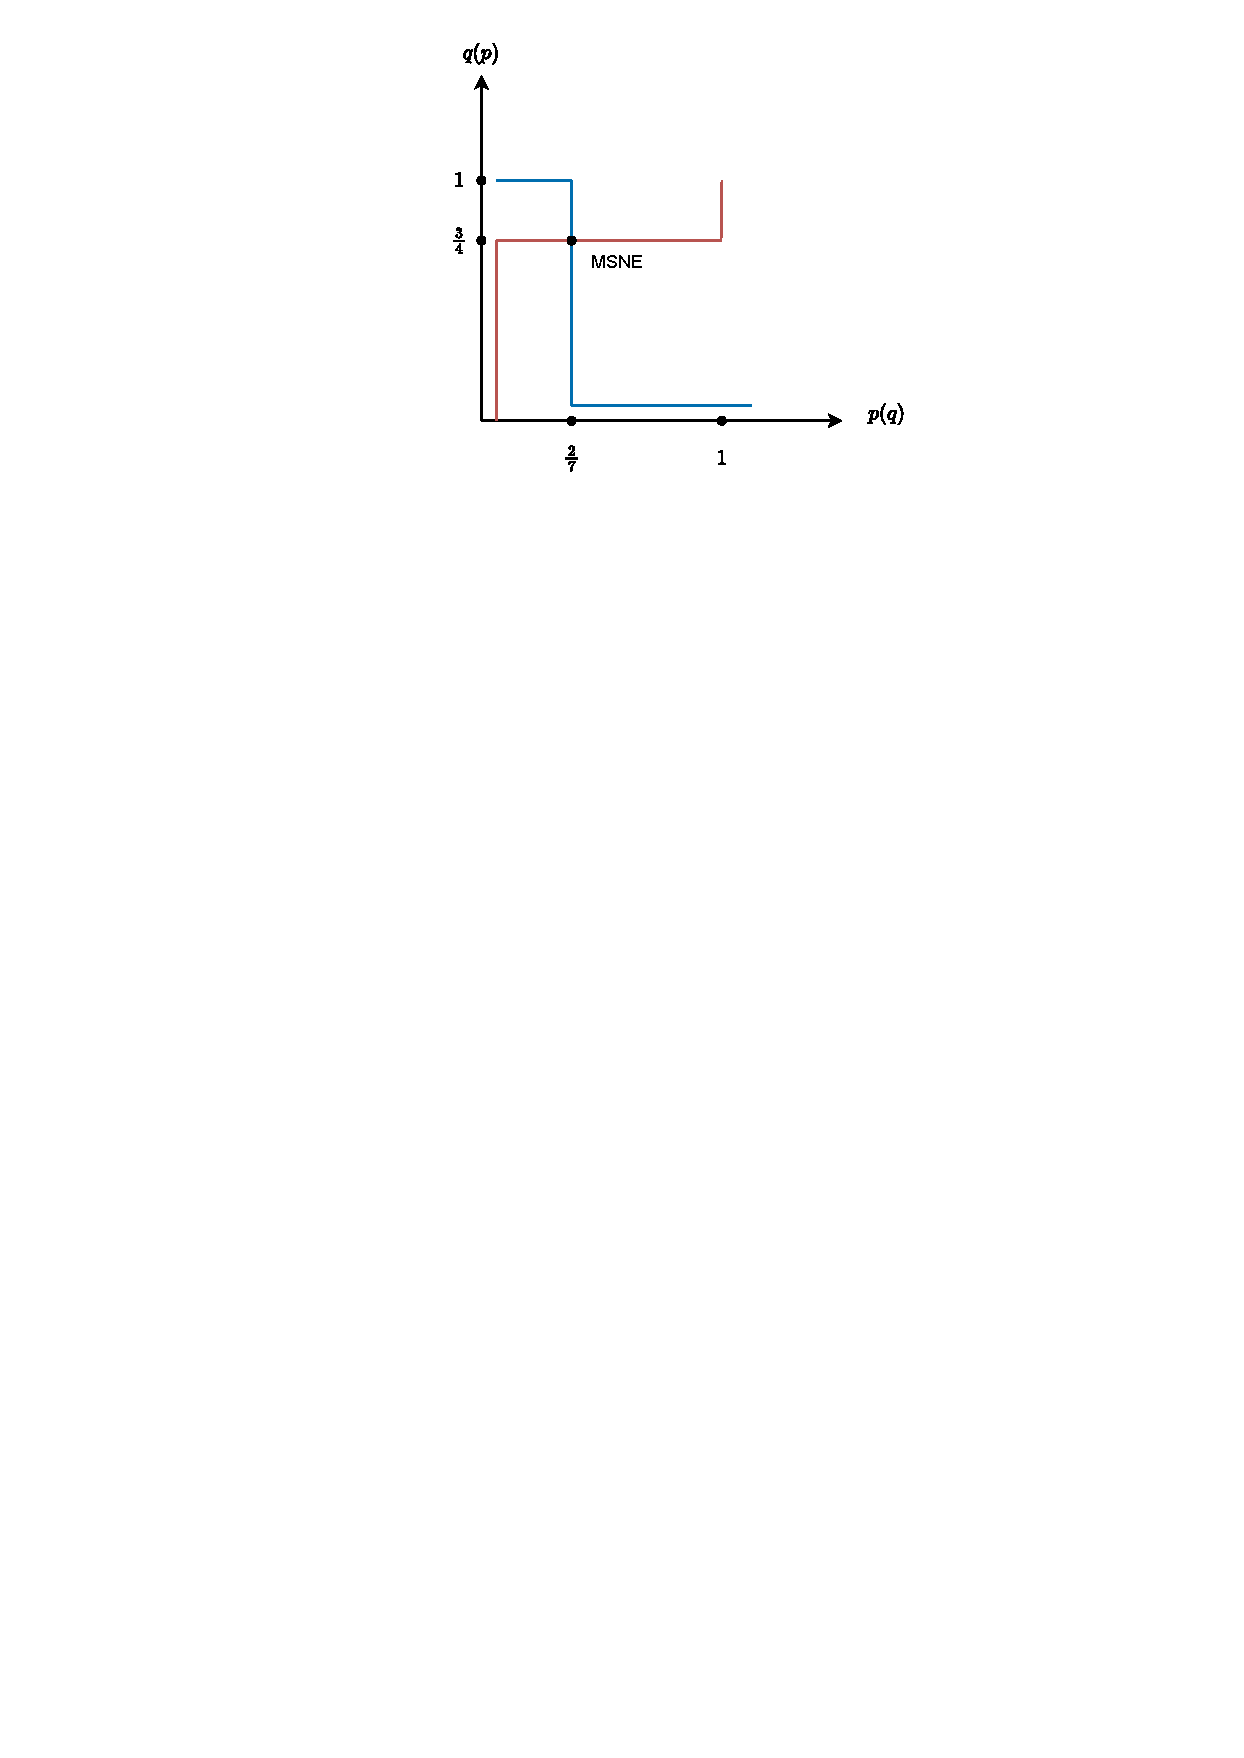
\includegraphics[width = \textwidth, trim = {4cm, 21cm, 3cm, 0cm}, clip]{document/0416.drawio.pdf}
\end{figure}
and one MSNE $\bar{x} = (\frac{2}{7}, \frac{5}{7})$, $\bar{y} = (\frac{3}{4}, \frac{1}{4})$. The NE payoffs for Alice and Bob are $\mathbb{E}_A(\frac{2}{7}, \frac{3}{4}) = \frac{7}{4}$, $\mathbb{E}_B(\frac{2}{7}, \frac{3}{4}) = -\frac{1}{7}$.

\begin{definition}
    The strategies $\alpha_{i_1}, \cdots, \alpha_{i_t}$ \uline{\textcolor{MarkerColour}{\textsc{strictly dominate}}} the strategy $\alpha_k\ (k\neq i_1, i_2, \cdots, i_t)$ if $\exists \gamma\in\Delta_t$, s.t. 
    \begin{align*}
        \gamma_1a_{i_i, j} + \cdots + \gamma_{t} a_{i_t, j} > a_{kj}, \ \forall 1\leqslant j\leqslant n
    \end{align*}

    We similar define $\beta_{j_1}, \cdots, \beta_{j_t}$ \uline{\textcolor{MarkerColour}{\textsc{strictly dominate}}} $\beta_l$.
\end{definition}

\setcounter{lemma}{2}
\begin{lemma}
    Suppose that in the game $(A, B)$, the strategies $\alpha_{i_1}, \cdots, \alpha_{i_t}$ strictly dominate the strategy $\alpha_k$. Then every MSNE $(\bar{x}, \bar{y})$ must have $\bar{x}_k =0$. Similarly, if $\beta_{j_1}, \cdots, \beta_{j_t}$ strictly dominates $\beta_l$, then every MSNE $(\bar{x}, \bar{y})$ must have $\bar{y}_l = 0$.
\end{lemma}
\begin{proof}
    By permuting the $\alpha_i$, we may assume $\alpha_1, \cdots, \alpha_t\ (1\leqslant t<m)$ strictly dominate $\alpha_m$. Then $\exists \gamma\in\Delta_t$, s.t. $\gamma_1a_{1j}+\cdots + \gamma_t a_{tj}>a_{mj}$, $\forall 1\leqslant j\leqslant n$. Suppose $\exists$ a MSNE $(\bar{x}, \bar{y})$ s.t. $\exists \bar{x}_m > 0$. Consider $x^{\prime}\in\Delta_m$ where
    \begin{align*}
        x_i^{\prime} = \left\lbrace\begin{array}{ll}
            x_1 + \varepsilon \gamma_i \bar{x}_m,  &\text{if} \ 1\leqslant i\leqslant t, \\
            \bar{x}_i & \text{if} \ t<i<m, \\
            (1-\varepsilon)\bar{x}_m & \text{if} \ i=m
        \end{array} \right.
    \end{align*}
    for some small $\varepsilon > 0$. Note that $x^{\prime}\in\Delta_m$ since $\bar{x}_m>0 \ \Longrightarrow$ $\bar{x}_i < 1$, $\forall 1\leqslant i\leqslant m$. Then
    \begin{align*}
        \mathbb{E}_A(x^{\prime}, \bar{y}) &= \sum\limits_{\substack{1\leqslant i\leqslant t, \\ 1\leqslant j\leqslant n}} a_{ij} (\bar{x}_i + \varepsilon \gamma_i \bar{x}_m) \bar{y}_i + \sum\limits_{\substack{t<i<m, \\ 1\leqslant j\leqslant n}} a_{ij} \bar{x}_i \bar{y}_j + \sum\limits_{1\leqslant j\leqslant n} a_{mj}(1-\varepsilon) \bar{x}_m \bar{y}_j \\
        & = \sum\limits_{\substack{1\leqslant i< m, \\ 1\leqslant j\leqslant n}} a_{ij}\bar{x}_i\bar{y}_j + \sum\limits_{1\leqslant j\leqslant n} a_{mj}(1-\varepsilon) \bar{x}_m\bar{y}_j + \sum\limits_{\substack{1\leqslant i\leqslant t, \\ 1\leqslant j\leqslant n}} a_{ij} \varepsilon \gamma_i \bar{x}_m\bar{y}_j \\
        & \underset{(*)}{>} \sum\limits_{\substack{1\leqslant i<m, \\ 1\leqslant j\leqslant n}}a_{ij}\bar{x}_i\bar{y}_j + \sum\limits_{1\leqslant j\leqslant n}a_{mj}(1-\varepsilon)\bar{x}_m\bar{y}_j  + \sum\limits_{1\leqslant j\leqslant n} a_{mj}\varepsilon \bar{x}_m\bar{y}_j = \mathbb{E}_A(\bar{x}, \bar{y})
    \end{align*}
    which contradicts that $\bar{x}$ is Alice's best response to $\bar{y}$.

   Note that $(*)$ holds since $\bar{x}_m\bar{y}_j > 0$ for some $j$. A similar proof holds if there is a strict domination among the $\beta_j$.
\end{proof}

\setcounter{example}{5}
\begin{example}\label{ex-5}
    Find the MSNEs of
    \begin{align*}
        \left(\begin{array}{ccc}
            (-1, -1) & (1, -2) & (5, 1)  \\
            (1, 2) & (2, 1) & (2, 4) \\
            (0, -2) & (1, -3) & (3, 2) \\
            (3, -2) & (4, 0) & (2, -2)
        \end{array} \right)
    \end{align*}
\end{example}

We say that $(\frac{1}{3}\times \mathrm{row}\ 1) + (\frac{2}{3}\times \mathrm{row}\ 4)$ and $(\frac{1}{2}\times\mathrm{row}\ 1)+ (\frac{1}{2}\times\mathrm{row}\ 4)$ strictly dominate rows $2$ and $3$. Delete row $2$ and $3$:
\begin{align*}
    \left(\begin{array}{ccc}
        (-1, -1) & (1, -2) & (5, 1)  \\
        (3, -2) & (4, 0) & (2, -2)
    \end{array} \right)
\end{align*}

Next, $(\frac{1}{2}\times\mathrm{column}\ 2) + (\frac{1}{2}\times\mathrm{column}\ 3)$ strictly dominates column 1. Delete column 1.

\begin{table}[H]
    \centering
    \begin{tabular}{|c|cc|}
    \hline
    & $y_2$ & $y_3$  \\ \hline
    $x_1$ & $(1,-2)$ & $(5, 1)$ \\
    $x_4$ & $(4, 0)$ & $(2, -2)$ \\ \hline
\end{tabular}
\end{table}

The surviving variables are $x_1$, $x_4$, $y_2$, $y_3$. Now proceed as in Example (\ref{ex-5}). Suppose Alice and Bob choose $\alpha_1$, $\beta_2$ with probabilities $p, q\in[0, 1]$. Then
\begin{align*}
    \mathbb{E}_A(p, q) &= pq + 5p(1-q) + 4(1-p)q + 2(1-p)(1-q) \\
    & = (-6q+3)p + (2q+2)
\end{align*}
\begin{align*}
    \Longrightarrow \text{Best response }p=\left\lbrace\begin{array}{ll}
        0,& \text{if} \ q>\frac{1}{2},  \\
        1,& \text{if} \ q<\frac{1}{2}, \\
        \in[0, 1],& \text{if} \ q = \frac{1}{2}. 
    \end{array} \right.
\end{align*}
\begin{align*}
    \mathbb{E}_B(p,q) &= -2pq + p(1-q) - 2(1-p)(1-q) \\
    & = (-5p+2)q + (3p-2)
\end{align*}
\begin{align*}
    \Longrightarrow \text{Best response }q=\left\lbrace\begin{array}{ll}
        0,& \text{if} \ q>\frac{2}{5},  \\
        1,& \text{if} \ q<\frac{2}{5}, \\
        \in[0, 1],& \text{if} \ q = \frac{2}{5}. 
    \end{array} \right.
\end{align*}

We have 
\begin{figure}[H]
    \centering
    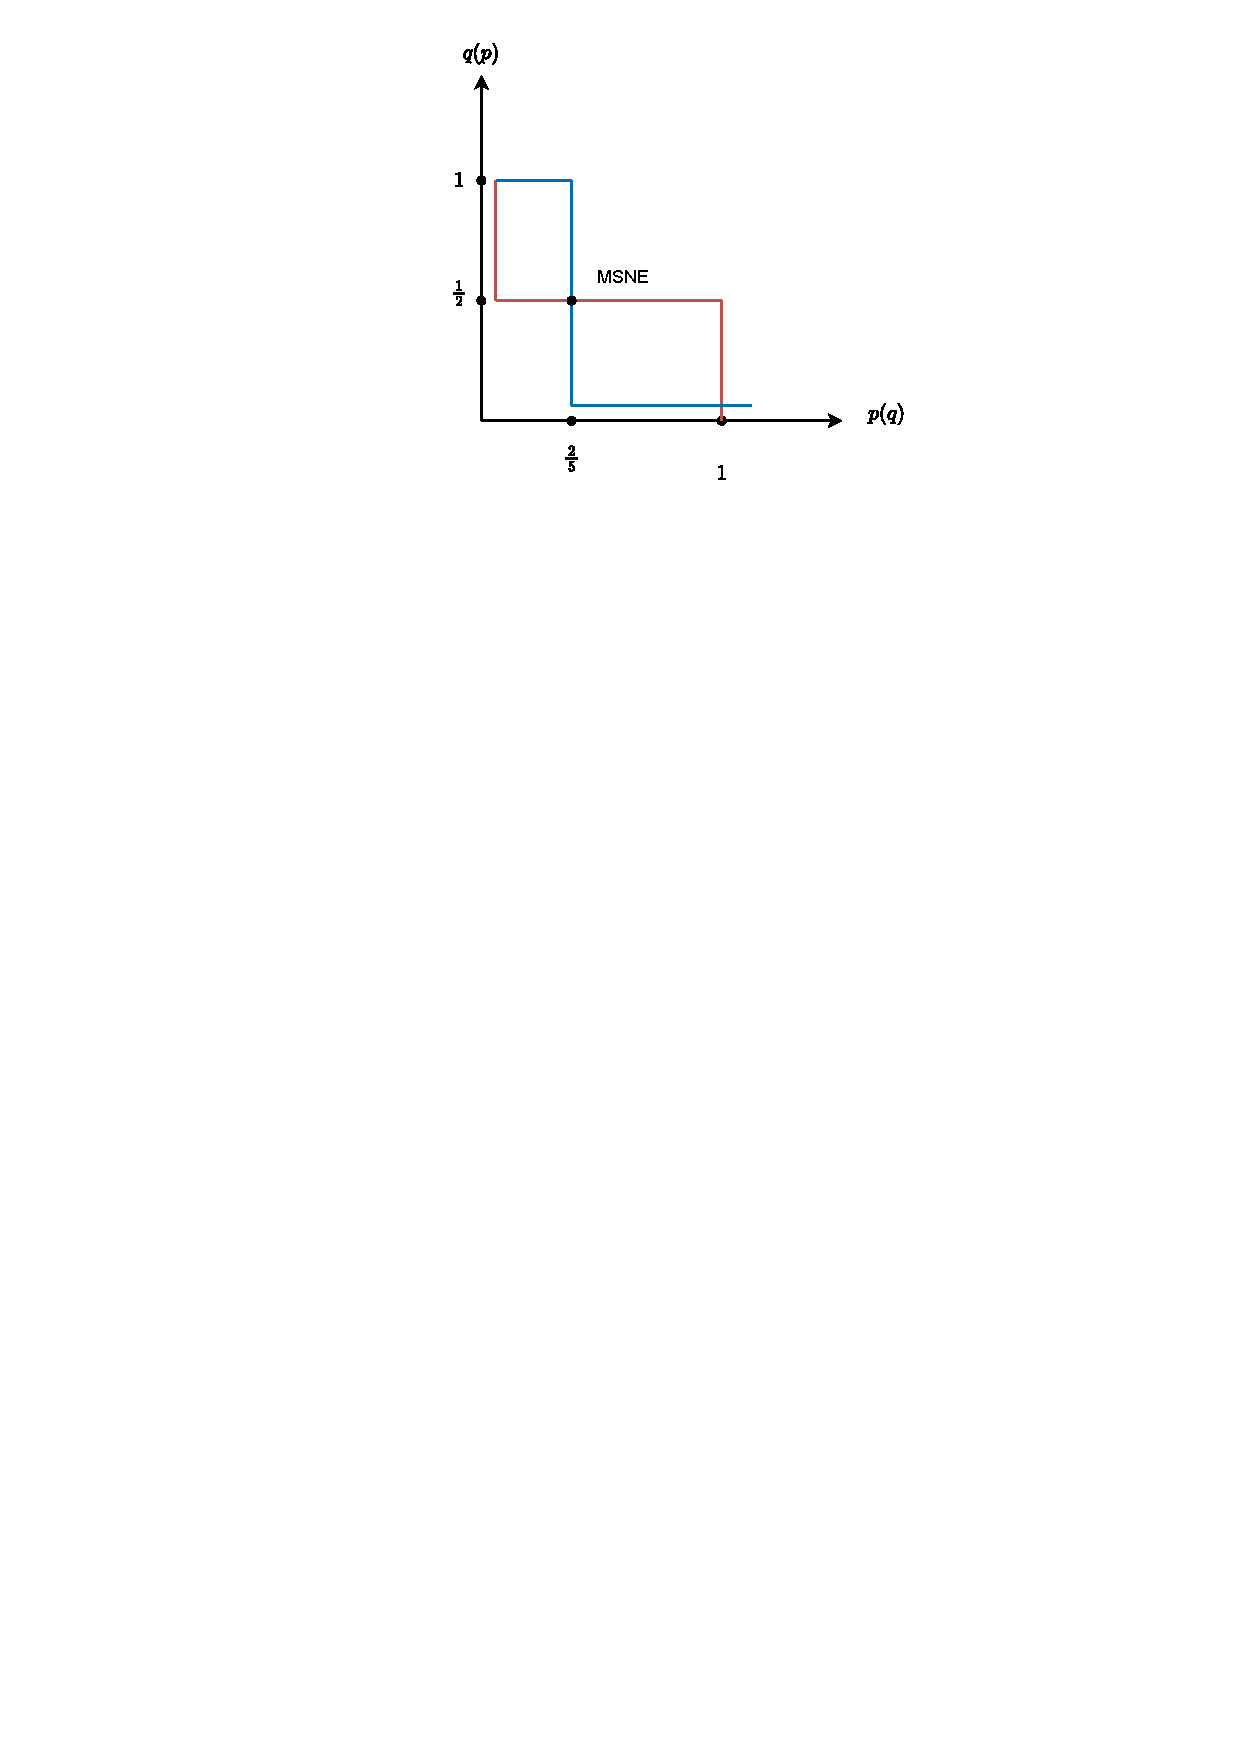
\includegraphics[width = 0.6\textwidth, trim = {4cm, 21cm, 3cm, 0cm}, clip]{document/0416.pdf}
\end{figure}

There are three MSNEs, two of which are also NEs.
\begin{table}[H]
    \centering
    \begin{tabular}{|c|c|c|c|}
    \hline
        \multirow{2}{*}{MSNE} & \multirow{2}{*}{NE} & \multicolumn{2}{c|}{NE payoffs} \\ \cline{3-4}
        & & Alice & Bob \\ \hline
        $\bar{x} = (0\ 0\ 0\ 1)^T$, $\bar{y} = (0\ 1\ 0)^T$ & $(4, 0)$ & $\mathbb{E}_A(0, 1) = 4$ & $\mathbb{E}_B(0, 1) = 0$ \\
        $\bar{x} = (1\ 0\ 0\ 0)^T$, $\bar{y} = (0\ 0\ 1)^T$ & $(5, 1)$ & $\mathbb{E}_A(1, 0) = 5$ & $\mathbb{E}_B(0, 1) = 1$ \\
        $\bar{x} = (\frac{2}{5}\ 0\ 0\ \frac{3}{5}$, $\bar{y} = (0\ \frac{1}{2}\ \frac{1}{2})^T$ & $\backslash$ & $\mathbb{E}_A(\frac{2}{5}, \frac{1}{2}) = 3$ & $\mathbb{E}_B(\frac{2}{5}, \frac{1}{2}) = -\frac{4}{5}$ \\ \hline
    \end{tabular}
\end{table}

\subsection{Cooperative Games}
For non-constant-sum games, it is interesting if the players can ``cooperate''.

\begin{example}
    Recall that in Prisoner's Dilemma, we have
    \begin{table}[H]
    \centering
    \begin{tabular}{|c|cc|}
        \hline
        \diagbox{Alice}{Bob}  &  $\beta_1 = $ Silent & $\beta_2 = $ Testify\\ \hline
        $\alpha_1 = $ Silent  & (-1, -1) & (-6, 0) \\
        $\alpha_2 = $ Testify & (0, -6) & (-3, 3) \\ \hline
    \end{tabular}
    \caption{(2.2)}
\end{table}
\end{example}
Suppose that, before being taken into separate rooms and questioned, Alice and Bob can communicate privately with each other. From the table (2.2), it seems a good compromise for them to both remain silence, so they each spend a short time of 1 year in jail.

\uline{\textcolor{MarkerColour}{\textsc{BUT}}}, can they keep their promise (cooperate) when they are questioned separately? If one of them decides to defect and testify (non-cooperate), while the other keeps the promise, the one who defects ``gains'' and does not go to jail, while the other is ``suckered'', and gets 6 years in jail. However, if they defect, then they are both worse off than if they had cooperated, since they each have to go to jail for 3 years ($3>1$).

We see that Prisoner's Dilemma is interesting since it asks the question ``Can Alice and Bob really trust each other?''.

In general, the payoff matrix may be represented as follows:
\begin{table}[H]
    \centering
    \begin{tabular}{|c|cc|}
        \hline
        \diagbox{Alice}{Bob} & C & NC \\ \hline
        C & $(r, r)$ & $(s, t)$ \\
        NC &$(t, s)$ & $(p, p)$ \\ \hline
    \end{tabular}
    {\hfill \begin{align*}
        \textrm{C} &= \textrm{Cooperate} \\
        \textrm{NC} &= \textrm{Non-Cooperate} \\
        \textrm{r} &= \textrm{Reward for cooperating} \\
        \textrm{t} &= \textrm{Temptation for defecting} \\
        \textrm{s} &= \textrm{Punishment for getting suckered} \\
        \textrm{p} &= \textrm{Punishment for non-cooperation}
    \end{align*}}
\end{table}

We see that $t$ and $s$ should be the largest and smallest payoffs. Also, for cooperation to be possible, we need $r>p$. Thus, $t>r>p>s$. We see that $(p, p)$ is the only NE. Moreover, by strict domination, we see that $\bar{x} = \bar{y} = (0\ 1)^T$ is the only MSNE, giving the NE payoffs $p, p$. Thus, it is wisest if they both defect.
\setcounter{example}{6}
\begin{example}[The game of Chicken]
    After a tough F1 race, Livid Lewis accuses Mad Max of cheating towards to win. Lewis promises Max that in the next race, he will cause a collision so that Max cannot win the race, he will cause a collision so that Max cannot win the race, to which Max replies that he will also promise to cause a collision.

    In the next race, the pair are side by side in their cars.
    \begin{itemize}
        \item In one of them swerves away\footnote{突然转向} to avoid a collision (``chickens\footnote{a man who is not brave} out''), and the other remains committed to the promise, the one who swerves is overtaken by the other. The score ``mind games points'' of $-3$ and $5$.
        \item If they both swerve, they both spin out of the race, and they each score $0$ mind games points.
        \item But is they both kept the promise, they cause a collision and each suffers an injury. They both score $-10$ mind games points.
    \end{itemize}

    The payoff matrix is 
    \begin{table}[H]
        \centering
        \begin{tabular}{|c|cc|}
            \hline
            \diagbox{Lewis}{Max} & Don't swerve & Swerve  \\ \hline
            Don't swerve & $(-10, -10)$ & $(5, -3)$ \\
            Swerve & $(-3, 5)$ & $(0, 0)$ \\ \hline
        \end{tabular}
    \end{table}

    We may generally represent the matrix as:
    \begin{table}[H]
        \centering
        \begin{tabular}{|c|cc|}
            \hline
            \diagbox{Lewis}{Max} & C & NC  \\ \hline
            C & $(r, r)$ & $(s, t)$ \\
            NC &$(t, s)$ & $(p, p)$ \\ \hline
        \end{tabular}
    \end{table}

    Clearly, $s$ and $r$ should be the largest and smallest payoffs. We should have $p>t$, since if one chickens out, it is better if the other chickens out than not. Thus $s>p>t>r$. We see that $(t, s)$ and $(s, t)$ are NEs. If say $s = 2$, $p = 1$, $t = -1$, $r = -M\ (M>0\text{ is large})$, then we can find that $\bar{x} = \bar{y} = \left( \frac{1}{M}, 1-\frac{1}{M}\right)$ is a MSNE. Thus it is wisest if they both swerve. 
\end{example}

\section{Games with t players}
Suppose $t\geqslant 2$ players play a game. Their strategy sets are $S_1, \cdots, S_t$. Let $S = S_1\times\cdots\times S_t$. The \uline{\textcolor{MarkerColour}{\textsc{payoff function}}} for Player $i\ (1\leqslant i\leqslant t)$ is $u_i:\ S\to\mathbb{R}$, where Player $i$ wins $u_i(s)$ when the strategies $s = (s_1,\cdots, s_t)\in S$ are chosen by the $t$ players. Thus for a 2-player game $(A, B)$, $u_1, u_2$ correspond to $A$, $B$.

We assume the players are non-cooperative, and they play rationally. Also, the sets $S_i$ are finite.
\begin{definition}
    $\bullet$ For $s\in S\ (1\leqslant i\leqslant t)$, write
    \begin{align*}
        s_{-i} = (s_1, \cdots, s_{i-1}, s_{i+1}, \cdots, s_t)\in S_1\times\cdots S_{i-1}\times S_{i}\times \cdots S_t
    \end{align*}

    For $s^{\prime}_i\in S_i$, write 
    \begin{align*}
        (s_i^{\prime}, s_{-i}) = (s_1, \cdots, s_{i-1}, s_i^{\prime}, s_{i+1}, \cdots, s_{t})\in S
    \end{align*}

    $\bullet$ A (pure strategy) Nash equilibrium (NE) is $\bar{s} \in S\ (\text{or}\ (u_1(\bar{s}), \cdots, u_t(\bar{s})))$ s.t.
    \begin{align*}
        u_i(\bar{s}) = u_i(\bar{s}_i, \bar{s}_{-i}) \geqslant u_i(s_i, \bar{s}_{-i}), \ \forall 1\leqslant i\leqslant t.
    \end{align*}

    Thus if Player $i$ changes strategy from a NE and all other players remain, then Player $i$ cannot win more.
\end{definition}

\begin{definition}
    \par $\bullet$ For probability distributions $\pi_i:S_i\to[0, 1]\ (1\leqslant i\leqslant t)$, the \uline{\textcolor{MarkerColour}{\textsc{expected utility}}} of Player $i$ is 
    \begin{align*}
        \mathbb{E}_i(\pi_1, \cdots, \pi_t) = \sum\limits_{s\in S} u_i(s) \prod\limits_{j=1}^t \pi_j(s_j).
    \end{align*}

    $\bullet$ $\bar{pi}_i$ is Player $i$'s best response to $\pi_1, \cdots, \pi_{i-1}, \pi_{i+1}, \cdots, \pi_t$ if 
    \begin{align*}
        \mathbb{E}_i(\pi_1, \cdots, \pi_{i-1}, \bar{\pi}_i, \pi_{i+1}, \cdots, \pi_t) \geqslant \mathbb{E}_i(\pi_1, \cdots, \pi_{i-1}, \pi_i, \pi_{i+1}, \cdots, \pi_t), \ \forall \pi_i
    \end{align*}

    $\bullet$ $(\bar{\pi}_1, \cdots, \bar{\pi}_t)$ is a \uline{\textcolor{MarkerColour}{\textsc{mixed strategy Nash equilibrium (MSNE)}}} if $\bar{\pi}_i$ is Player $i$'s best response to $\bar{\pi}_1, \cdots, \bar{\pi}_{i-1}, \bar{\pi}_{i+1}, \cdots, \bar{\pi}_t, \ \forall 1\leqslant i\leqslant t$. The \uline{\textcolor{MarkerColour}{\textsc{Nash equilibrium payoff}}} for Player $i$ is $\mathbb{E}_i(\bar{\pi}_1, \cdots, \bar{\pi}_t)$.
\end{definition}

\begin{example}
    Suppose we have a 3-player game, where $S_1=\{\alpha_1, \alpha_2\}$, $S_2 = \{\beta_1, \beta_2\}$, $S_3 = \{\gamma_1, \gamma_2\}$, and 
    \begin{table}[H]
        \centering
        \begin{tabular}{|c|cc|}
            \hline
            \diagbox{$P_1$}{$P_2$} & $\beta_1$ & $\beta_2$  \\ \hline
            $\alpha_1$ & $(3, 3, 3)$ & \boxed{$(3, 4, 3)$} \\
            $\alpha_2$ & \boxed{$(4, 3, 3)$} & $(1, 1, 0)$ \\ \hline
        \end{tabular}
        \caption{If $P_3$ choose $\gamma_1$}
    \end{table}

    \begin{table}[H]
        \centering
        \begin{tabular}{|c|cc|}
            \hline
            \diagbox{$P_1$}{$P_2$} & $\beta_1$ & $\beta_2$  \\ \hline
            $\alpha_1$ & \boxed{$(3, 3, 4)$} & $(0, 1, 1)$ \\
            $\alpha_2$ & $(1, 0, 1)$ & \boxed{$(1, 1, 1)$} \\ \hline
        \end{tabular}
        \caption{If $P_3$ choose $\gamma_3$}
    \end{table}
\end{example}

There are four NEs as indicated. Now consider mixed strategies. Let $x = (p, 1-p), \ y=(q, 1-q),\ z = (r, 1-r)$, be the probability distributions.
\begin{align*}
    \mathbb{E}_1(p, q, r) &= \left[3qr + 3(1-q)r + 3q(1-r)p\right]p \\
    & + \left[4qr+(1-q)r+q(1-r)+(1-q)(1-r)\right](1-p) \\
    &= (3qr+3r-6qr-1)p + (3qr+1) 
\end{align*}
\begin{align*}
    \Longrightarrow \text{Best response }p = \left\lbrace\begin{array}{ll}
        0, & \text{if} \ 3qr+3r-6qr-1<0 (*) \\
        1, & \text{if} \ 3qr+3r-6qr-1>0 \\
        \in[0, 1], & \text{if} \ 3qr+3r-6qr-1=0
    \end{array}\right.
\end{align*}

Similarly (by symmetry of $p, q, r$)
\begin{align*}
    \Longrightarrow \text{ BR }q & = \left\lbrace\begin{array}{ll}
        0, & \text{if} \  3p+3r-6pr-1 < 0 \\
        1, & \text{if} \  3p+3r-6pr-1 > 0  \\
        \in[0, 1] & \text{if} \ 3p+3r-6pr-1 = 0 
    \end{array} \right. \\
    \Longrightarrow \text{ BR }r & = \left\lbrace\begin{array}{ll}
        0, & \text{if} \  3p+3q-6pq-1 < 0 \\
        1, & \text{if} \  3p+3q-6pq-1 > 0  \\
        \in[0, 1] & \text{if} \ 3p+3q-6pq-1 = 0 
    \end{array} \right.
\end{align*}

Let $(\bar{x}, \bar{y}, \bar{z})$ be a MSNE. If $\bar{p} = 0$, 
\begin{align*}
    \text{BR }q &= \left\lbrace\begin{array}{ll}
        0, &\text{if} \ r<\frac{1}{3}  \\
        1, &\text{if} \ r>\frac{1}{3} \\
        \in[0, 1], & \text{if}\ r= \frac{1}{3}
    \end{array} \right. ,\\
    \text{BR }e &= \left\lbrace\begin{array}{ll}
        0, &\text{if} \ q<\frac{1}{3}  \\
        1, &\text{if} \ q>\frac{1}{3} \\
        \in[0, 1], & \text{if}\ q= \frac{1}{3}
    \end{array} \right. .
\end{align*}

\begin{figure}[H]
    \centering
    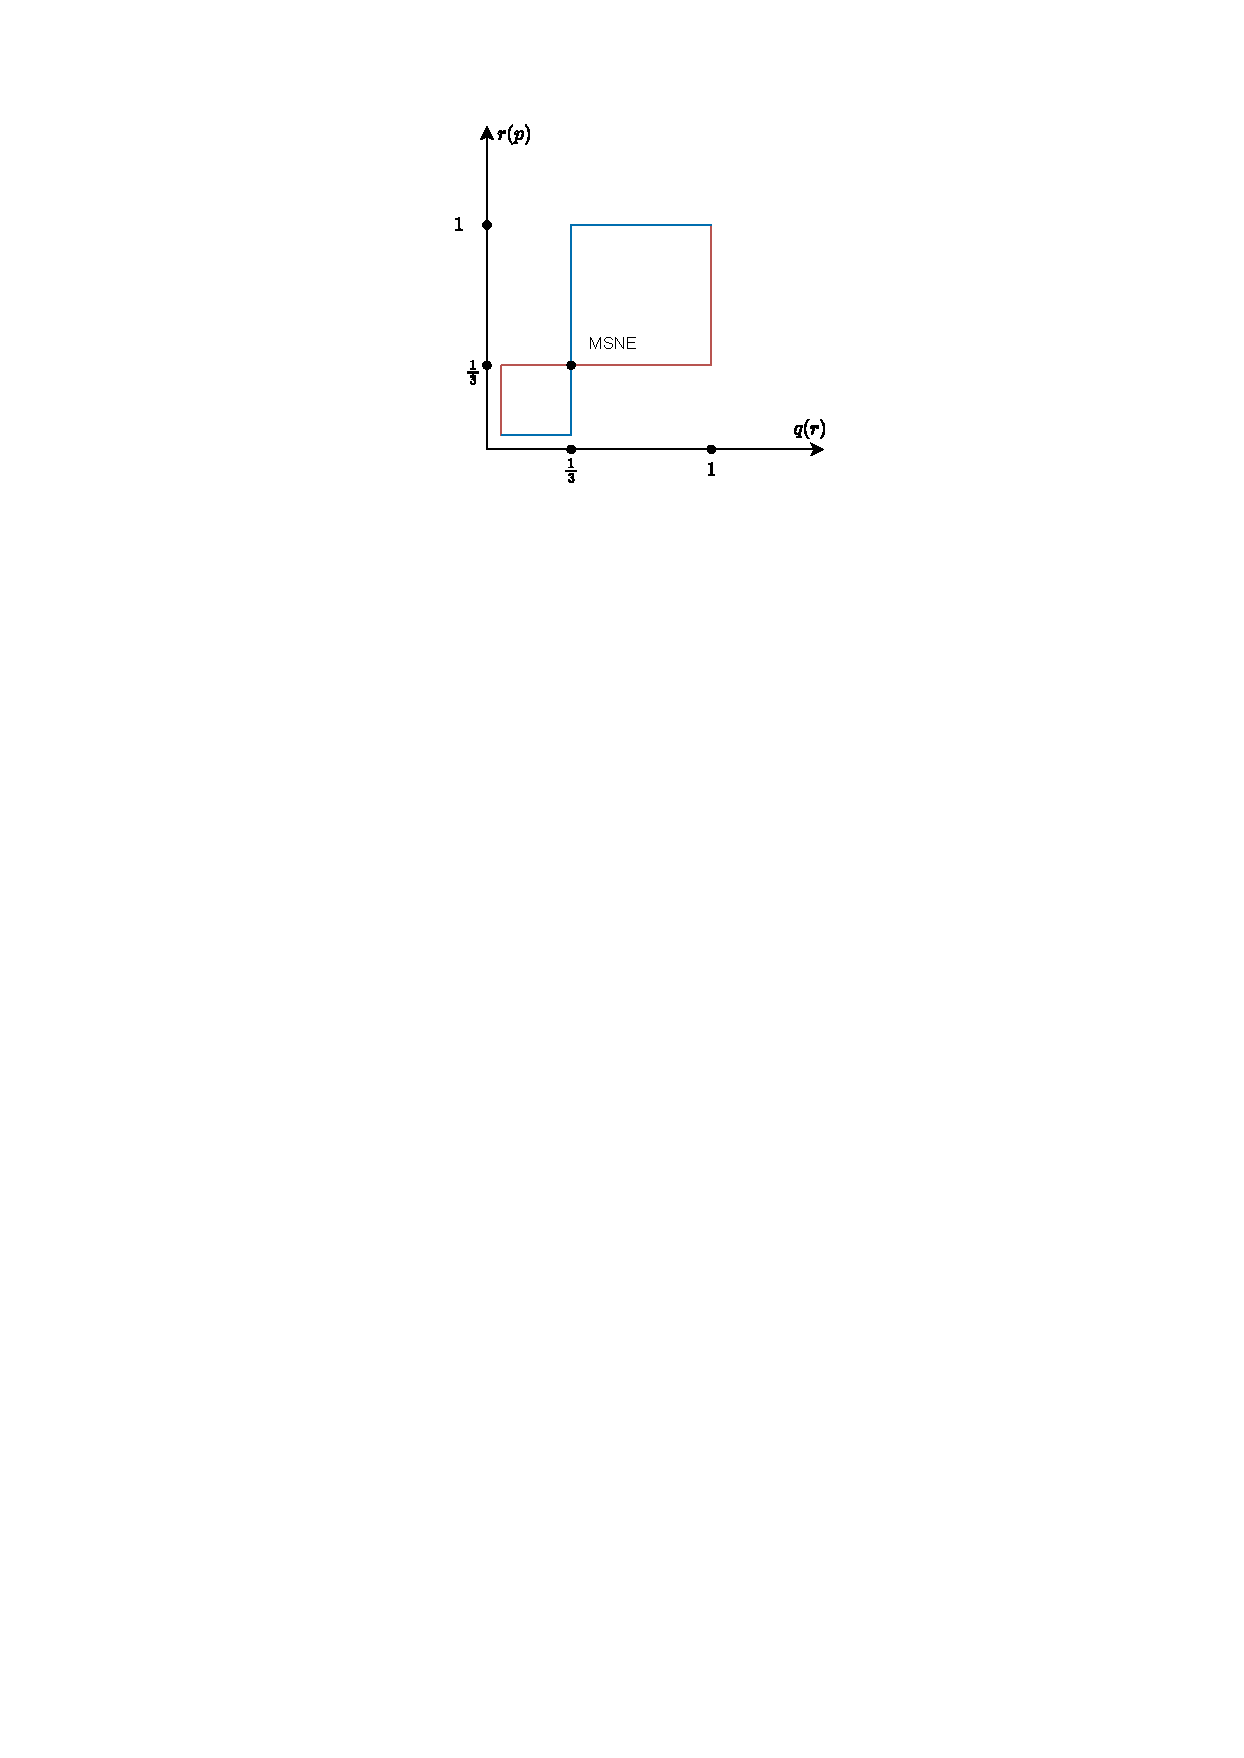
\includegraphics[width = 0.6\textwidth, trim = {4cm, 21cm, 3cm, 2cm}, clip]{document/0423.pdf}
\end{figure}

$\Longrightarrow$ $(p, q, r) = (0, 0, 0),\ (0, \frac{1}{3}, \frac{1}{3}), \ (0, 1, 1)$. We discord $(0, \frac{1}{3}, \frac{1}{3})$ since it does not satisfy (*). If $\bar{p} = 1$,
\begin{align*}
    \text{BR }q &= \left\lbrace\begin{array}{ll}
        0, & \text{if} \ r>\frac{2}{3} \\
        1, & \text{if} \ r<\frac{2}{3} \\
        \in[0, 1], &\text{if} \ r = \frac{2}{3}
    \end{array}\right. ,\\
    \text{BR }r &= \left\lbrace\begin{array}{ll}
        0, & \text{if} \ q>\frac{2}{3} \\
        1, & \text{if} \ q<\frac{2}{3} \\
        \in[0, 1], &\text{if} \ q = \frac{2}{3}
    \end{array}\right. 
\end{align*}
\begin{figure}[H]
    \centering
    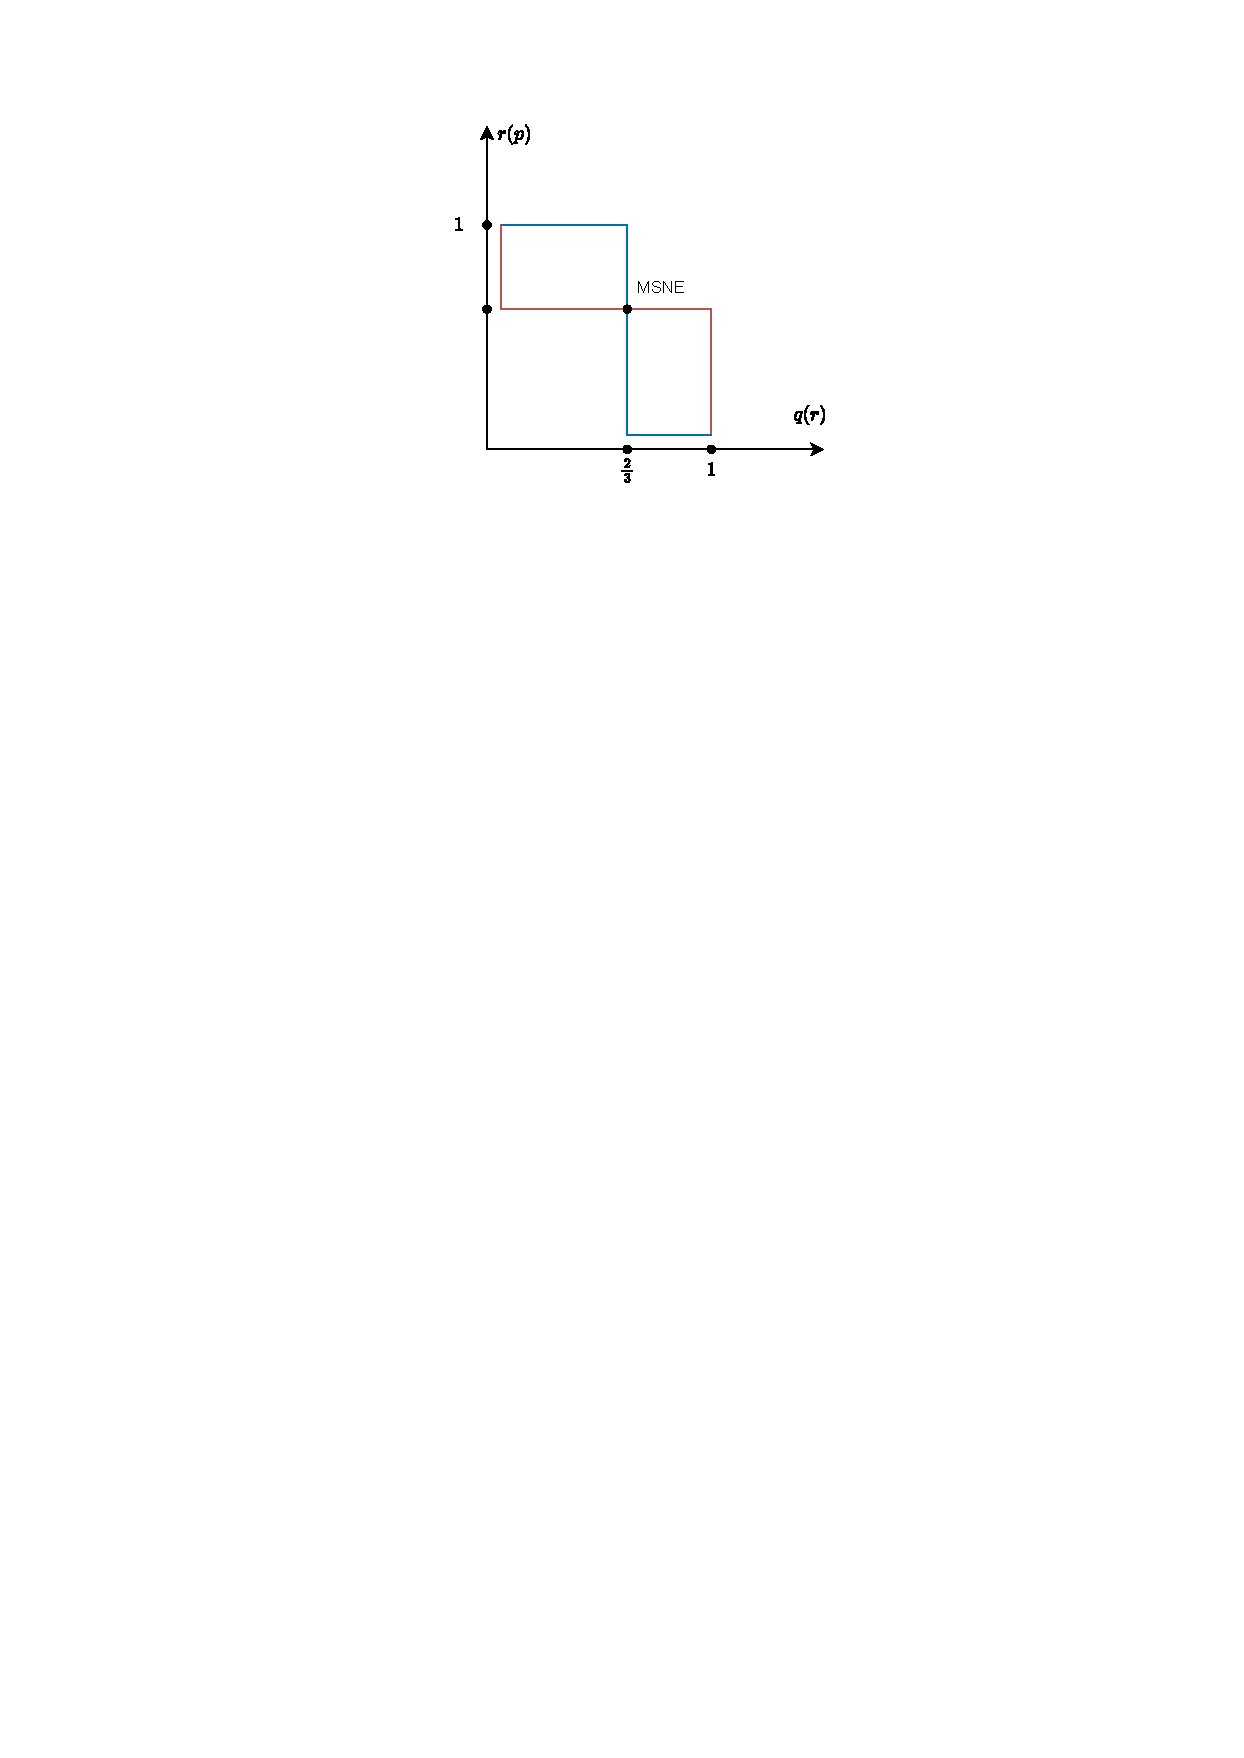
\includegraphics[width = 0.6\textwidth, trim = {4cm, 21cm, 3cm, 2cm}, clip]{document/0423-1.pdf}
\end{figure}
$\Longrightarrow\ (\bar{p}, \bar{q}, \bar{r}) = (1, 0, 1),\ (1, \frac{2}{3}, \frac{2}{3}), \ (1, 1, 0)$.

Now by symmetry of $p, q, r$, suppose $\bar{p}, \bar{q}, \bar{r} \in (0, 1)$. Then 
\begin{align*}
    &3q+3r-6qr-1 = 0 {\hfill\quad (1)} \\
    &3p+3r-6pr-1=0 {\hfill\quad (2)} \\
    &3p+3q-6pq-1=0 {\hfill\quad (3)}
\end{align*}
$(1), (2)\Longrightarrow\ 3q-6qr = 3p-6pr \Longrightarrow \ (p-q)(1-2r) = 0$.

$\bullet$ If $p=q$, $(3)\Longrightarrow\ 6p-6p^2-1=0\Longrightarrow \ \bar{p}=\bar{q} = \frac{3\pm \sqrt{3}}{6}\in(0, 1)$.

$(1)\Longrightarrow\ \bar{p} = \bar{q} = \bar{r} = \frac{3\pm\sqrt{3}}{6}\in(0, 1)$.

$\bullet$ If $r = \frac{1}{2}$, $(1) \Longrightarrow \ \frac{1}{2} = 0$, which is absurd.

\paragraph{Conclusion}
\par NEs: $(\bar{p}, \bar{q}, \bar{r}) = (0, 0, 0),\ (0, 1, 1), \ (1, 0, 1), \ (1, 1, 0)$.
\par MSNEs: $(\bar{p}, \bar{q}, \bar{r}) = (1, \frac{2}{3}, \frac{2}{3}),\ (\frac{2}{3}, 1, \frac{2}{3}),\ (\frac{2}{3}, \frac{2}{3}, 1), \ \left(\frac{3\pm\sqrt{3}}{6}, \frac{3\pm\sqrt{3}}{6}, \frac{3\pm\sqrt{3}}{6}\right)$.

We may obtain all possible $(\bar{x}, \bar{y}, \bar{z})$ and NE payoffs from these.

We have the celebrated result.

\setcounter{theorem}{3}
\begin{theorem}[Nash's theorem]\label{Th 2.4}
    If a game with $t\geqslant 2$ players has finite strategy sets $S_1, \cdots, S_t$ then $\exists$ MSNE.
\end{theorem}

Note that \ref{Th 2.4} says that a MSNE exists, but does not tell us how to find one!

A proof of Th \ref{Th 2.4} requires:
\begin{theorem}[Brouwer's fixed-point theorem]\label{Th 2.5}
    Let $K\subset \mathbb{R}^n$ be a compact, convex set, and $f:K\to K$ be continuous. Then $\exists x\in K$, s.t. $f(x) = x$. Such an $x$ is a \uline{\textcolor{MarkerColour}{\textsc{fixed point}}}.
\end{theorem}

\begin{proof}
    For Th \ref{Th 2.4} (Using Th \ref{2.5})

   First, consider the case of two players Alice and Bob, with matrices $A, B\in\mathbb{R}^{m\times n}$. Let $K = \Delta_m\times \Delta_n$. For $(x, y)\in K$, we define $f(x, y) = (x^{\prime}, y^{\prime})$ as follows. Let
   \begin{align*}
       c_i = c_i(x, y) = \max\left(A_i y - x^T Ay, 0 \right), \ 1\leqslant i\leqslant m
   \end{align*}
    where $A_i$ is the $i^{\text{th}}$ row of $A$. Note that $c_i$ is Alice's possible gain by switching from mixed strategy $x$ to pure strategy $\alpha_i$, if such a gain is positive. Let $x^{\prime}\in\Delta_m$ where 
    \begin{align*}
        x_i^{\prime} = \dfrac{x_i + c_i}{1+\sum\limits_{k=1}^m c_k}
    \end{align*}

    Similarly, let
    \begin{align*}
        d_j = d_j(x, y) = \max\left( x^T B^j - x^T B y, 0\right), \ 1\leqslant j\leqslant n
    \end{align*}
    where $B^j$ is the $j^{\text{th}}$ column of $B$, and let $y^{\prime}\in \Delta_n$, where
    \begin{align*}
        y_j^{\prime} = \dfrac{y_j+d_j}{1+ \sum\limits_{k=1}^n d_k}.
    \end{align*}

    Now, if $c_i = 0$ (or $x^TAy\geqslant A_iy)$, $\forall i$, then $x^{\prime} = x$ is a best response to $y$. Otherwise, $c = \sum\limits_{i=1}^m c_i >0$. Then 
    \begin{align*}
        \sum\limits_{i=1}^m c_i A y &> cx^TAy = \sum\limits_{i=1}^m c_ix^TAy \\
        \Longrightarrow \ \sum\limits_{i=1}^m (x_i+c_i) y &> (1+c)x^TAy \\
        \Longrightarrow \ \sum\limits_{i=1}^m x_i^{\prime} A_i y &> x^TAy
    \end{align*}
   so $x^{\prime}$ is a better response to $y$ than $x$ is. Similarly, either $y^{\prime} = y$ is a best response to $x$, or $y^{\prime}$ is a better response to $x$ than $y$ is.

   Clearly, $K$ is compact and convex, and $f$ is continuous since $c_i$ and $d_j$ are. Thus Th \ref{Th 2.5} $\Longrightarrow \ f$ has a fixed point, which is a MSNE.

   For $t\geqslant 3$ players, we define for Player $j$ with pure strategy $l$, the quantity $c_l^{(i)}$, which is the gain that Player $j$ gets by switching from current strategy $x^{(j)}$ to pure strategy $l$, is positive, while fixing the current strategies of all other players. The argument is similar.
\end{proof}

\chapter{Graph Theory and Networks}
\section{Terminology}
A \uline{\textcolor{MarkerColour}{\textsc{graph}}} is a pair $G = (V, E)$ where $V$ is a set, and $E$ is a set of ordered pairs from $V$.

For example

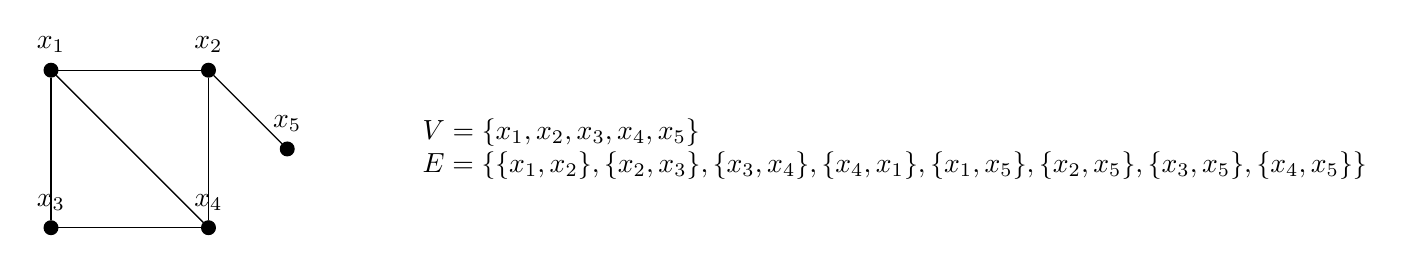
\begin{tikzpicture}
  % 定义点
  \node[circle,draw,fill=black,label=above:$x_1$,minimum size=5pt,inner sep=0pt] (x1) at (0,0) {};
  \node[circle,draw,fill=black,label=above:$x_2$,minimum size=5pt,inner sep=0pt] (x2) at (2,0) {};
  \node[circle,draw,fill=black,label=above:$x_3$,minimum size=5pt,inner sep=0pt] (x3) at (0,-2) {};
  \node[circle,draw,fill=black,label=above:$x_4$,minimum size=5pt,inner sep=0pt] (x4) at (2,-2) {};
  \node[circle,draw,fill=black,label=above:$x_5$,minimum size=5pt,inner sep=0pt] (x5) at (3,-1) {};

  % 定义边
  \draw (x1) -- (x2);
  \draw (x2) -- (x4);
  \draw (x1) -- (x3);
  \draw (x3) -- (x4);
  \draw (x1) -- (x4);
  \draw (x4) -- (x1);
  \draw (x2) -- (x5);

  \node[align=left, right=of x5, xshift=5mm]{
    $V = \{x_1, x_2, x_3, x_4, x_5\}$ \\
    $E = \{\{x_1, x_2\}, \{x_2, x_3\}, \{x_3, x_4\}, \{x_4, x_1\}, \{x_1, x_5\}, \{x_2, x_5\}, \{x_3, x_5\}, \{x_4, x_5\}\}$
  };
\end{tikzpicture}


$V$ is the \uline{\textcolor{MarkerColour}{\textsc{Vertex set}}} and $E$ is the \uline{\textcolor{MarkerColour}{\textsc{edge set}}}. We may also write $V(G)$ and $E(G)$ for $V$ and $E$. $|V|$ and $|E|$ are the \uline{\textcolor{MarkerColour}{\textsc{order}}} and \uline{\textcolor{MarkerColour}{\textsc{size}}} of $G$.

Note: No loops.

No multi edges.

\paragraph{Important examples:}

The \uline{\textcolor{MarkerColour}{\textsc{empty graph}}} $E_n$ of order $n$:

\begin{tikzpicture}
  % 定义点
  \node[circle,draw,fill=black,label=above:$x_1$,minimum size=5pt,inner sep=0pt] (x1) at (0,0) {};
  \node[circle,draw,fill=black,label=above:$x_2$,minimum size=5pt,inner sep=0pt] (x2) at (2,0) {};
  \node[circle,draw,fill=black,label=above:$x_3$,minimum size=5pt,inner sep=0pt] (x3) at (0,-2) {};
  \node[circle,draw,fill=black,label=above:$x_n$,minimum size=5pt,inner sep=0pt] (xn) at (2,-2){};

  \node[align=left, right=of x5, xshift=20mm]{
    $V = \{x_1, \cdots , x_n\}$
  };
\end{tikzpicture}

The \uline{\textcolor{MarkerColour}{\textsc{complete graph}}} $K_n$ of order n:

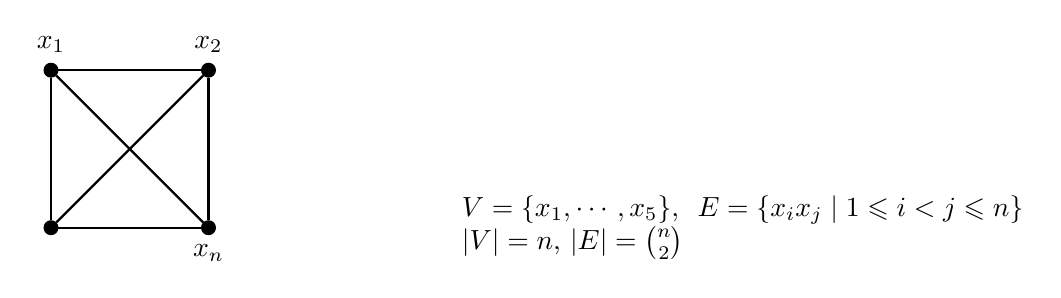
\begin{tikzpicture}
  % 定义样式
  \tikzset{vertex/.style = {circle, draw, fill=black, minimum size=5pt, inner sep=0pt}}
  \tikzset{edge/.style = {draw, thick}}

  % 定义点
  \node[vertex, label=above:$x_1$] (x1) at (0,0) {};
  \node[vertex, label=above:$x_2$] (x2) at (2,0) {};
  \node[vertex, label=below:$x_n$] (x3) at (2,-2) {};
  \node[vertex, label=below:] (x4) at (0,-2) {};

  % 定义边
  \draw[edge] (x1) -- (x2);
  \draw[edge] (x1) -- (x3);
  \draw[edge] (x1) -- (x4);
  \draw[edge] (x2) -- (x3);
  \draw[edge] (x2) -- (x4);
  \draw[edge] (x3) -- (x4);

  \node[align=left, right=of x3, xshift=20mm]{
    $V = \{x_1, \cdots,  x_5\}$, \ $E = \{x_ix_j\mid 1\leqslant i<j\leqslant n \}$ \\
    $|V| = n$,\ $|E| =\binom{n}{2}$
  };
\end{tikzpicture}

The \uline{\textcolor{MarkerColour}{\textsc{path}}} $P_n$ of order $n$, \uline{\textcolor{MarkerColour}{\textsc{length}}} $n-1$:

\usetikzlibrary{positioning, shapes.misc}
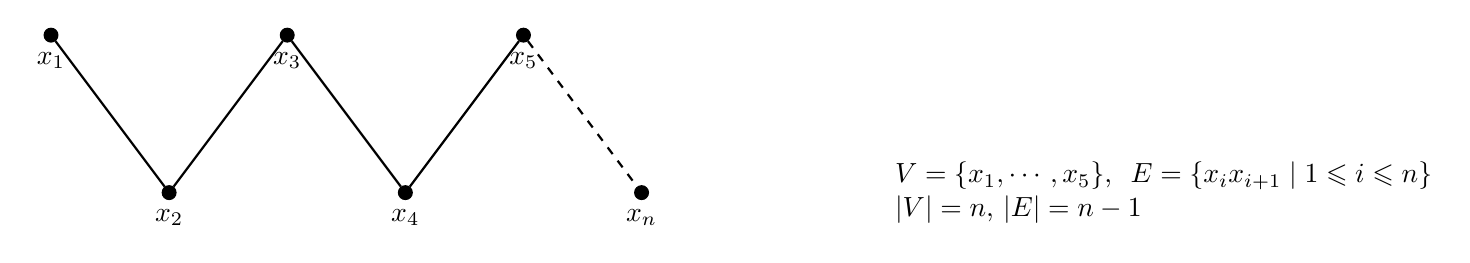
\begin{tikzpicture}
  % 定义样式
  \tikzset{vertex/.style = {circle, draw, fill=black, minimum size=5pt, inner sep=0pt}}
  \tikzset{edge/.style = {draw, thick}}
  \tikzset{dots/.style = {draw, thick, dashed}}

  % 定义点
  \node[vertex, label=below:$x_1$] (x1) at (0,1) {};
  \node[vertex, label=below:$x_2$] (x2) at (1.5,-1) {};
  \node[vertex, label=below:$x_3$] (x3) at (3,1) {};
  \node[vertex, label=below:$x_4$] (x4) at (4.5,-1) {};
  \node[vertex, label=below:$x_5$] (x5) at (6,1) {};
  \node[vertex, label=below:$x_n$] (xn) at (7.5,-1) {}; % Assuming x_n is x_6

  % 定义边
  \draw[edge] (x1) -- (x2);
  \draw[edge] (x2) -- (x3);
  \draw[edge] (x3) -- (x4);
  \draw[edge] (x4) -- (x5);
  \draw[dots] (x5) -- (xn); % Dashed line for ellipsis
    
    \node[align=left, right=of xn, xshift=20mm]{
    $V = \{x_1, \cdots,  x_5\}$, \ $E = \{x_ix_{i+1}\mid 1\leqslant i\leqslant n \}$ \\
    $|V| = n$,\ $|E| =n-1$
  };
\end{tikzpicture}

We may write $P_n = x_1x_2\cdots x_n$. We say that $x_1, x_n$ are the \uline{\textcolor{MarkerColour}{\textsc{end-vertices}}} of $P_n$, and $P_n$ is an \uline{\textcolor{MarkerColour}{\textsc{$x_1-x_n$ Path}}}.

The \uline{\textcolor{MarkerColour}{\textsc{cycle}}} $C_n$ of order and length $n\geqslant 3$: 
\usetikzlibrary{shapes.geometric, positioning, decorations.markings}

\begin{tikzpicture}
  % 定义半径和中心点
  \def\radius{1.5cm} % 半径为2cm
  \def\center{0,0} % 中心点为原点

  % 使用极坐标定义六边形的六个顶点
  \foreach \x/\angle in {1/0, 2/60, 3/120, 4/180, 5/240, n/300}
    \node[fill, circle, inner sep=2pt, label={[font=\small]\angle:$x_{\x}$}] (x\x) at ([shift={(\angle:\radius)}]\center) {};

  % 连接顶点
  \draw (x1) -- (x2) -- (x3) -- (x4) -- (x5) -- (xn) -- (x1) -- cycle;

  \node[align=left, right=of x1, xshift=20mm]{
    $V = \{x_1, \cdots,  x_n\}$, \ $E = \{x_ix_{i+1}\mid 1\leqslant i\leqslant n \}\cup\{x_nx_1\}$ \\
    $|V| = n$,\ $|E| =n$
  };
\end{tikzpicture}

We may write $C_n = x_1x_2\cdots x_nx_1$.

The \uline{\textcolor{MarkerColour}{\textsc{complete bipartite graph}}} $K_{m, n}$:

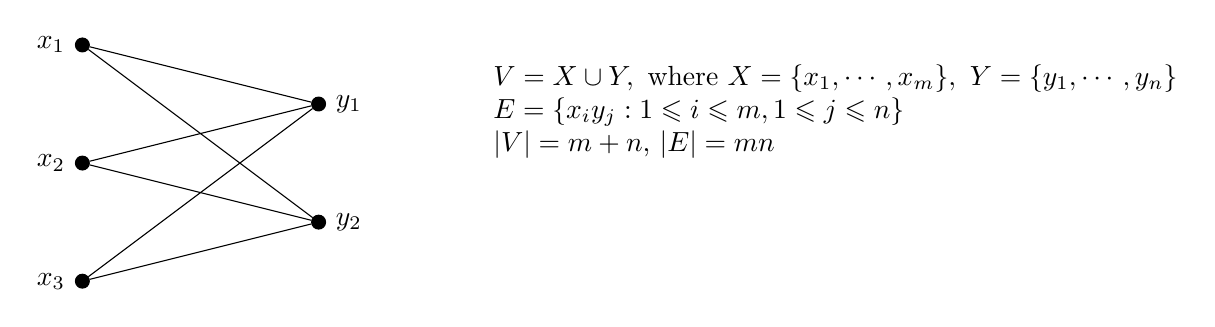
\begin{tikzpicture}[scale=1.5, vertex/.style={circle, draw, fill=black, minimum size=5pt, inner sep=0pt}]

  % 定义左侧顶点
  \node[vertex, label=left:$x_1$] (x1) at (0,2) {};
  \node[vertex, label=left:$x_2$] (x2) at (0,1) {};
  \node[vertex, label=left:$x_3$] (x3) at (0,0) {};

  % 定义右侧顶点
  \node[vertex, label=right:$y_1$] (y1) at (2,1.5) {};
  \node[vertex, label=right:$y_2$] (y2) at (2,0.5) {};

  % 绘制边连接顶点
  \foreach \i in {1,2,3}
    \foreach \j in {1,2}
      \draw (x\i) -- (y\j);

    \node[align=left, right=of y1, xshift=10mm, yshift=-1mm]{
    $V = X\cup Y,\ \text{where}\ X = \{x_1, \cdots, x_m\},\ Y = \{y_1, \cdots, y_n\}$ \\
    $E = \{x_iy_j:1\leqslant i\leqslant m, 1\leqslant j\leqslant n\}$ \\
    $|V| = m+n$, $|E| = mn$
  };
\end{tikzpicture}

In general, a graph $G = (V, E)$ is \uline{\textcolor{MarkerColour}{\textsc{bipartite}}} if we have $V = X\cup Y$ s.t. $E\subset \{xy\mid x\in X, y\in Y\}$.

$G^{\prime} = (V^{\prime}, E^{\prime})$ is a \uline{\textcolor{MarkerColour}{\textsc{subgraph}}} of $G = (V, E)$, written $G^{\prime}\subset G$, if $V^{\prime}\subset V$ and $E^{\prime}\subset E$. If $V^{\prime} = V$ and $E^{\prime}\subset E$, then $G^{\prime}$ is a \uline{\textcolor{MarkerColour}{\textsc{spanning subgraph}}} of $G$.

Let $G = (V, E)$. If $xy\in E$, then $x$ and $y$ are \uline{\textcolor{MarkerColour}{\textsc{neighbours}}} or \uline{\textcolor{MarkerColour}{\textsc{adjacent}}}. The \uline{\textcolor{MarkerColour}{\textsc{neighbourhood}}} of $x\in V$ is $\Gamma(x)$ (or $N(x)$) $=\{y\in V\mid xy\in E\}$. The \uline{\textcolor{MarkerColour}{\textsc{degree}}} of $x$ is $d(x) = |\Gamma(x)|$.

\begin{definition}[Directed Graph]
    A \uline{\textcolor{MarkerColour}{\textsc{directed graph}}} or \uline{\textcolor{MarkerColour}{\textsc{digraph}}} is a pair $D = (V, A)$, where $V$ is a set and $A$ is a set of ordered pairs from $V$.
\end{definition}

For example:

\usetikzlibrary{decorations.markings}
\begin{tikzpicture}[arrow1/.style={postaction={decorate}, decoration={
        markings,
        mark=at position 0.5 with {\arrow{stealth}} % 在中间位置添加箭头
    }},
    vertex/.style={circle, draw, fill=black, minimum size=5pt, inner sep=0pt}
]

  % 节点样式定义
  \tikzstyle{vertex} = [circle, draw, fill=black, minimum size=5pt, inner sep=0pt]

  % 定义节点
  \node[vertex, label=above:$x_1$] (x1) at (0,0) {};
  \node[vertex, label=above:$x_2$] (x2) at (2,0) {};
  \node[vertex, label=below:$x_3$] (x3) at (0,-2) {};
  \node[vertex, label=below:$x_4$] (x4) at (2,-2) {};
  \node[vertex, label=right:$x_5$] (x5) at (3,-1) {};

  % 绘制有向边
  \draw[arrow1] (x1) -- (x2);
  \draw[arrow1] (x4) -- (x2);
  \draw[arrow1] (x5) -- (x2);
  \draw[arrow1] (x4) -- (x3);

  % 绘制弧线
  \draw[arrow1, bend right] (x1) to (x3);
  \draw[arrow1, bend right] (x3) to (x1);
  \draw[arrow1, bend right] (x1) to (x4);
  \draw[arrow1, bend right] (x4) to (x1);

  % 绘制更复杂的弧线,比如回环
  % \draw[->, loop above] (x2) to (x2);
  \node[align=left, right=of x5, xshift=20mm]{
    $V = \{x_1, \cdots,  x_5\}$,\\
    $E = \{x_1x_2, x_1x_3, x_1x_4, x_3x_1, x_4x_1, x_4x_2, x_4x_3, x_5x_2 \}$
  };
\end{tikzpicture}

$V$ is the \uline{\textcolor{MarkerColour}{\textsc{vertex set}}}, and $A$ is the \uline{\textcolor{MarkerColour}{\textsc{arc set}}}. We may also write $V(D)$ and $A(D)$ for $V$ and $A$. $|V|$ and $|A|$ are the \uline{\textcolor{MarkerColour}{\textsc{order}}} and \uline{\textcolor{MarkerColour}{\textsc{size}}} of $D$.

Note: No loops.

No multiple arcs. But $x1-x2, x2-x1$ is acceptable.

\begin{example}
    The \uline{\textcolor{MarkerColour}{\textsc{complete diagraph}}} $K_n$ of order $n$:

\begin{tikzpicture}[
    arrow in middle/.style={postaction={decorate}, decoration={
        markings,
        mark=at position 0.5 with {\arrow{stealth}}
    }},
    vertex/.style={circle, draw, fill=black, minimum size=5pt, inner sep=0pt}
]

  % 定义顶点位置
  \node[vertex, label=above:$x_1$] (x1) at (0,2) {};
  \node[vertex, label=above:$x_2$] (x2) at (2,2) {};
  \node[vertex, label=below:] (x3) at (0,0) {};
  \node[vertex, label=below:$x_n$] (x4) at (2,0) {};

  % 绘制有向边
  \foreach \from/\to in {x1/x2, x2/x3, x3/x4, x4/x1, x1/x3, x2/x4}
    \draw[arrow in middle] (\from) -- (\to);
  \foreach \from/\to in {x2/x1, x3/x2, x4/x3, x1/x4, x3/x1, x4/x2}
    \draw[arrow in middle, bend left=20] (\from) to (\to);

    \node[align=left, right=of x2, xshift=20mm, yshift = -4mm]{
    $V = \{x_1, \cdots,  x_n\}$,\\
    $E = \{x_ix_j\mid 1\leqslant i \neq j \leqslant n\}$ \\
    $|V| = n$, $|A| = n(n_1)$
  };
\end{tikzpicture}
\end{example}

\begin{example}
    The \uline{\textcolor{MarkerColour}{\textsc{directed path}}}, or \uline{\textcolor{MarkerColour}{\textsc{path}}} $\hat{P}_n$ of order $n$, length $n-1$:

    \vspace{0.5cm}
    \begin{tikzpicture}[
    arrow in middle/.style={postaction={decorate}, decoration={
        markings,
        mark=at position 0.5 with {\arrow{stealth}}
    }},
    vertex/.style={circle, draw, fill=black, minimum size=5pt, inner sep=0pt}
]
  % 定义样式
  \tikzset{vertex/.style = {circle, draw, fill=black, minimum size=5pt, inner sep=0pt}}
  \tikzset{edge/.style = {draw, thick}}
  \tikzset{dots/.style = {draw, thick, dashed}}

  % 定义点
  \node[vertex, label=below:$x_1$] (x1) at (0,1) {};
  \node[vertex, label=below:$x_2$] (x2) at (1.5,-1) {};
  \node[vertex, label=below:$x_3$] (x3) at (3,1) {};
  \node[vertex, label=below:$x_4$] (x4) at (4.5,-1) {};
  \node[vertex, label=below:$x_5$] (x5) at (6,1) {};
  \node[vertex, label=below:$x_n$] (xn) at (7.5,-1) {}; % Assuming x_n is x_6

  % 定义边
  \draw[arrow in middle] (x1) -- (x2);
  \draw[arrow in middle] (x2) -- (x3);
  \draw[arrow in middle] (x3) -- (x4);
  \draw[arrow in middle] (x4) -- (x5);
  \draw[dots] (x5) -- (xn); % Dashed line for ellipsis
    
    \node[align=left, right=of xn, xshift=3mm, yshift = 4mm]{
    $V = \{x_1, \cdots,  x_5\}$, \\
    $E = \{x_ix_{i+1}\mid 1\leqslant i\leqslant n \}$, \\
    $|V| = n$,\ $|E| =n-1$
  };
\end{tikzpicture}

We may write $\hat{P}_n = x_1x_2\cdots x_n$. We say that $x_1, x_n$ are the \uline{\textcolor{MarkerColour}{\textsc{source}}} and \uline{\textcolor{MarkerColour}{\textsc{sink}}} of $\hat{P}_n$, and $\hat{P}_n$ is an $x_1 - x_n$ Path.
\end{example}

\begin{example}
    The \uline{\textcolor{MarkerColour}{\textsc{directed cycle}}}, or \uline{\textcolor{MarkerColour}{\textsc{dicycle}}} $\hat{C}_n$ of order and length $n\geqslant 3$ (Sometimes $n=2$ are allowed).

    \begin{tikzpicture}[
    arrow in middle/.style={postaction={decorate}, decoration={
        markings,
        mark=at position 0.5 with {\arrow{stealth}}
    }},
    vertex/.style={circle, draw, fill=black, minimum size=5pt, inner sep=0pt}
]
  % 定义半径和中心点
  \def\radius{1.5cm} % 半径为2cm
  \def\center{0,0} % 中心点为原点

  % 使用极坐标定义六边形的六个顶点
  \foreach \x/\angle in {1/0, 2/60, 3/120, 4/180, 5/240, n/300}
    \node[fill, circle, inner sep=2pt, label={[font=\small]\angle:$x_{\x}$}] (x\x) at ([shift={(\angle:\radius)}]\center) {};

  % 连接顶点
  \draw[arrow in middle] (x1) -- (x2) -- (x3) -- (x4) -- (x5) -- (xn) -- (x1);

  \node[align=left, right=of x1, xshift=20mm]{
    $V = \{x_1, \cdots,  x_n\}$, \ $E = \{x_ix_{i+1}\mid 1\leqslant i\leqslant n \}\cup\{x_nx_1\}$ \\
    $|V| = n$,\ $|E| =n$
  };
\end{tikzpicture}

We may write $\hat{C}_n = x_1x_2\cdots x_nx_1$. 
\end{example}

$D^{\prime} = (V^{\prime}, A^{\prime})$ is a \uline{\textcolor{MarkerColour}{\textsc{subdigraph}}} of $D = (V, A)$, written $D^{\prime}\subset D$, if $V^{\prime}\subset V$ and $A^{\prime} \subset A$. If $V^{\prime} = V$ and $A^{\prime}\subset A$, then $D^{\prime}$ is a \uline{\textcolor{MarkerColour}{\textsc{spanning subdigraph}}} of $D$.

Let $D = (V, A)$. If $xy\in A$, then $Y$ is an \uline{\textcolor{MarkerColour}{\textsc{out-neighbour}}} of $x$ and $x$ is an \uline{\textcolor{MarkerColour}{\textsc{in-neighbour}}} of $y$. The \uline{\textcolor{MarkerColour}{\textsc{out-neighbourhood/in-neighbourhood}}} of $x\in V$ are $\Gamma^{+}(x) = \{y\in V: xy\in A\}$ and $\Gamma^{-}(x) = \{y\in V: yx\in A\}$. The \uline{\textcolor{MarkerColour}{\textsc{out-degree/in-degree}}} of $x\in V$ are $d^+(x) = |\Gamma^+(x)|$ and $d^-(x) = |\Gamma^-(x)|$.

For a digraph $D = (V, A)$, the \uline{\textcolor{MarkerColour}{\textsc{underlying graph}}} is $G = (V, E)$ where $E = \{xy\mid xy\in A\ or\ yx\in A\}$.

A graph $G = (V, E)$ is \uline{\textcolor{MarkerColour}{\textsc{connected}}} if $\forall x, y\in V$, $\exists x-y$ path $P\subset G$. A digraph $D = (V, A)$ is \uline{\textcolor{MarkerColour}{\textsc{connected}}} if the underlying graph of $D$ is connected, and \uline{\textcolor{MarkerColour}{\textsc{strong-connected}}} if $\forall x, y\in V$, $\exists x-y$ path $\hat{P}\subset D$.

\uline{\textcolor{MarkerColour}{\textsc{A network graph}}} is a pair $(G, w)$, where $G$ is a graph, and $w\mid E(G)\to\mathbb{R}$. A \uline{\textcolor{MarkerColour}{\textsc{network digraph}}} is a pair $(D, w)$, where $D$ is a digraph, and $w\mid A(D)\to\mathbb{R}$. In each case, $w$ is a \uline{\textcolor{MarkerColour}{\textsc{weight function}}}.

From now on, we assume $V$ is finite, $\forall$ graphs and digraphs. In many situations, we consider connected graphs and digraphs.

\section{Shortest path problem}
\begin{definition}
    Let $(D, w)$ be a network digraph and $x, y\in V(D)$. A \uline{\textcolor{MarkerColour}{\textsc{walk}}} from $x$ to $y$, or an \uline{\textcolor{MarkerColour}{\textsc{$x-y$ walk}}}, is a sequence vertices $x = v_0, v_1, \cdots, v_k = y$ s.t. $v_{i-1}v_i\in A(D)$, $\forall 1\leqslant i\leqslant k$. Note that $v_0, v_1, \cdots, v_k$ and $v_0 v_1 \cdots v_{k-1} v_k$ are not necessarily distinct.
\end{definition}

\vspace{0.5cm}
\begin{tikzpicture}[
    arrow in middle/.style={postaction={decorate}, decoration={
        markings,
        mark=at position 0.5 with {\arrow{stealth}}
    }},
    vertex/.style={circle, draw, fill=black, minimum size=5pt, inner sep=0pt}
]
  % 定义样式
  \tikzset{vertex/.style = {circle, draw, fill=black, minimum size=5pt, inner sep=0pt}}
  \tikzset{edge/.style = {draw, thick}}
  \tikzset{dots/.style = {draw, thick, dashed}}

    \node[vertex, label=left:$x_1$](x1) at (0, 0) {};
    \node[vertex, label=below:](x2) at (1, 0) {};
    \node[vertex, label=below:](x3) at (2, 0) {};
    \node[vertex, label=below:](x4) at (3, 0) {};
    \node[vertex, label=below:](x5) at (4, 0) {};
    \node[vertex, label=below:$y$](x6) at (8, 0) {};
    \node[vertex, label=below:](x7) at (4, 2) {};
    \node[vertex, label=below:](x8) at (6, 2) {};
    \node[vertex, label=below:](x9) at (8, 2) {};

    \draw[arrow in middle] (x1) -- (x2) -- (x3) -- (x4) -- (x5) -- (x6);
    \draw[arrow in middle] (x5) to[out=90, in=180] (x7)
                               to[out=0, in=180] (x8)
                               to[out=0, in=180] (x9)
                               to[out=0, in=90] (x6);
\end{tikzpicture}

We say that $y$ is \uline{\textcolor{MarkerColour}{\textsc{reachable}}} from $x$ if $\exists$ an $x-y$ walk (equivalently, $\exists x-y$ path) in $D$. In this case, a \uline{\textcolor{MarkerColour}{\textsc{shortest path}}} from $x$ to $y$ is an $x-y$ walk. $x = v_0,v_1,\cdots, v_k =y$ with minimum weight, that is, $\sum\limits_{i=1}^k w(v_{i-1}, v_i)$ is minimum. Note that $D$ is strong connected $\Longleftrightarrow$ \ $y$ is reachable from $x$, $\forall\ x, y\i V(D)$.

We consider the following problem.
\subsection{Problem 3.1 Shortest path problem}
Let $(D, w)$ be a network digraph. Let $x\in V(D)$ s.t. $\forall \ y\in V(D)\backslash \{x\}$, $y$ is reachable from $x$. Find a shortest path from $x$ to every $y\in V(D)\backslash \{x\}$. We call $x$ the \uline{\textcolor{MarkerColour}{\textsc{source vertex}}}.

We consider two algorithms for solving Problem 3.1.
\subsubsection{A. Dijkstra's Algorithm}
We assume $w: A(D)\to \mathbb{R}_{\geqslant 0}$ in Problem 3.1. As Dijkstra's Algorithm is performed, every vertex $y\in V(D)$ is given a temporary label $T(y)$ which gets updated, then eventually a permanent label $P(y)$, which will be the weight of a shortest path from $x$ to $y$. Then algorithm is as follows.

\paragraph{1.} Set $P(x) = 0$, and
\begin{align*}
    T(y) = \left\lbrace\begin{array}{ll}
        w(xy), &\ \text{if} \ y\in \Gamma^+(x)  \\
        \infty, &\ \text{if} \ y\in V(D)\backslash \{\Gamma^+(x)\cup\{x\}\}
    \end{array} \right.
\end{align*}

Then, choose $y\in\Gamma^+(x)$ with $T(y)$ minimum, and set $P(y) = T(y)$.

\paragraph{2} Now, suppose $z\in V(D)$ is the most recent vertex to receive a permanent label, that is, to have $P(z)$ defined. $\forall v\in \Gamma^+(z)$ s.t. $T(v)$ but not $P(v)$ is defined, update
\begin{align*}
    T(v) = \min\left( T(v), P(z) + w(zv)\right)
\end{align*}

Then $\forall u\in V(D)$ s.t. $T(u)$ but not $P(u)$ is defined, choose $y$ where $T(y)$ is minimum, and set $P(y) = T(y)$. 

\paragraph{3} Return to Step $2$. Repeat procedure until termination.

\begin{remark}
    \begin{itemize}
        \item In Step 1 and 2 if there is a tie for the minimum, we may not choose any such suitable $y$.
        \item The assumption $w: A(D) \to \mathbb{R}_{\geqslant 0}$ implies that any shortest path from $x$ is in fact a path.
    \end{itemize}
\end{remark}

\setcounter{example}{0}
\begin{example}
    Find the shortest paths from $x_1$ to all other vertices, where $(D, w)$ is:
    \begin{tikzpicture}[
    arrow in middle/.style={postaction={decorate}, decoration={
        markings,
        mark=at position 0.5 with {\arrow{stealth}}
    }},
    vertex/.style={circle, draw, fill=black, minimum size=5pt, inner sep=0pt}
]

  % 定义顶点位置
  \node[vertex, label=above:$x_1$] (x1) at (0,0) {};
  \node[vertex, label=above:$x_2$] (x2) at (2,2) {};
  \node[vertex, label=below:$x_3$] (x3) at (4,2) {};
  \node[vertex, label=below:$x_4$] (x4) at (2,0) {};
  \node[vertex, label=below:$x_5$] (x5) at (4,0) {};
  \node[vertex, label=below:$x_6$] (x6) at (6,0) {};
  \node[vertex, label=below:$x_7$] (x7) at (3,-2) {};
    
  % 绘制有向边并添加数字标签
  \draw[arrow in middle] (x1) to [bend right=20] node[midway, above, sloped] {5} (x2);
  \draw[arrow in middle] (x2) to [bend right=20] node[midway, above, sloped] {1} (x1);

  % 其他连线,如果需要标注也可以添加
  \draw[arrow in middle] (x6) to [bend right=20] node[midway, below, sloped] {0} (x7);
  \draw[arrow in middle] (x7) to [bend right=20] node[midway, below, sloped] {2} (x6);  % 替换“标签”为实际数值

  \draw[arrow in middle] (x1) -- (x4) node[midway, above, sloped] {2};
  \draw[arrow in middle] (x4) -- (x5) node[midway, above, sloped] {0};
  \draw[arrow in middle] (x5) -- (x6) node[midway, above, sloped] {9};
  \draw[arrow in middle] (x4) -- (x2) node[midway, above, sloped] {2};
  \draw[arrow in middle] (x5) -- (x2) node[midway, above, sloped] {1};

  \draw[arrow in middle] (x2) -- (x3) node[midway, above, sloped] {6};
  \draw[arrow in middle] (x1) -- (x7) node[midway, above, sloped] {5};
  \draw[arrow in middle] (x3) -- (x6) node[midway, above, sloped] {1};
  %\draw[arrow in middle] (x4) -- (x2) node[midway, above, sloped] {2};
  
\end{tikzpicture}
\end{example}

We initially set 
\begin{table}[H]
    \centering
    \begin{tabular}{|ccccccc|}
    \hline
       $x_1$ & $x_2$ & $x_3$ & $x_4$ & $x_5$ & $x_6$ & $x_7$   \\ \hline
    \uline{$0^*$} & 5 & $\infty$ & $2^{\boxed{*}}$ & $\infty$ & $\infty$ & 5 \\ \hline
    \end{tabular}
\end{table}
where $\_$ means the out-neighbour of this vertex (z in Step 2) are being considered, and ${}^*$ is a permanent label, with $^{\boxed{*}}$ the newest one. The next iteration is 
\begin{table}[H]
    \centering
    \begin{tabular}{|ccccccc|}
    \hline
       $x_1$ & $x_2$ & $x_3$ & $x_4$ & $x_5$ & $x_6$ & $x_7$   \\ \hline
    $0^*$ & 4 & $\infty$ & \uline{$2^*$} & $2^{\boxed{*}}$ & $\infty$ & 5 \\ \hline
    \end{tabular}
\end{table}

New temporary labels:
\begin{align*}
    x_2: & \min(5, 2+2) = 4\\
    x_5: & \min(\infty, 2+0) = 2
\end{align*}

$2 = \min(4, 2, 5)$, this becomes permanent.

Repeating, we obtain:
\begin{table}[H]
    \centering
    \begin{tabular}{|ccccccc|}
    \hline
       $x_1$ & $x_2$ & $x_3$ & $x_4$ & $x_5$ & $x_6$ & $x_7$   \\ \hline
    $0^*$ & $3^{\boxed{*}}$ & $\infty$ & $2^*$ & \uline{$2^*$} & $5$ & 5 \\
    $0^*$ & \uline{$3^*$} & $9$ & $2^*$ & $2^*$ & $5^{\boxed{*}}$ & 5 \\
    $0^*$ & $3^*$ & $9$ & $2^*$ & $2^*$ & \uline{$5^*$} & $5^{\boxed{*}}$ \\
    $0^*$ & $3^*$ & $9^{\boxed{*}}$ & $2^*$ & $2^*$ & $5^*$ & \uline{$5^{*}$} \\
    \hline
    \end{tabular}
\end{table}

We obtain a \uline{shortest paths tree from $x_1$ as}:

\begin{tikzpicture}[
    arrow in middle/.style={postaction={decorate}, decoration={
        markings,
        mark=at position 0.5 with {\arrow{stealth}}
    }},
    vertex/.style={circle, draw, fill=black, minimum size=5pt, inner sep=0pt}
]

  % 定义顶点位置
  \node[vertex, label=above:$x_1$] (x1) at (0,0) {};
  \node[vertex, label=above:$x_2$] (x2) at (2,2) {};
  \node[vertex, label=below:$x_3$] (x3) at (4,2) {};
  \node[vertex, label=below:$x_4$] (x4) at (2,0) {};
  \node[vertex, label=below:$x_5$] (x5) at (4,0) {};
  \node[vertex, label=below:$x_6$] (x6) at (6,0) {};
  \node[vertex, label=below:$x_7$] (x7) at (3,-2) {};
  
  \draw[arrow in middle] (x1) -- (x4) node[midway, above, sloped] {2};
  \draw[arrow in middle] (x4) -- (x5) node[midway, above, sloped] {0};
  \draw[arrow in middle] (x5) -- (x6) node[midway, above, sloped] {9};
  % \draw[arrow in middle] (x4) -- (x2) node[midway, above, sloped] {2};
  \draw[arrow in middle] (x5) -- (x2) node[midway, above, sloped] {1};

  \draw[arrow in middle] (x2) -- (x3) node[midway, above, sloped] {6};
  \draw[arrow in middle] (x1) -- (x7) node[midway, above, sloped] {5};
  % \draw[arrow in middle] (x3) -- (x6) node[midway, above, sloped] {1};
  % \draw[arrow in middle] (x4) -- (x2) node[midway, above, sloped] {2};
  
\end{tikzpicture}

To obtain a shortest path from $x_1$ to $y$, look at when $y$ is given ${}^{\boxed{*}}$, and backtrack.

\begin{theorem}
    Let $(D, w)$ be a network digraph, where $w:A(D)\to\mathbb{R}_{\geqslant 0}$. Then Dijkstra's Algorithm solves Problem 3.1.
\end{theorem}
\begin{proof}
    Let $R_t\subset V(D)$ be the set of permanently labelled vertices after $t$ iterations of Dijkstra's Algorithm. Note that $R_t = R_{t-1}\cup\{y\}$, where $y$ becomes permanently labelled at the $t^{th}$ iteration ($1<t\leqslant |V(D)|$). We use induction on $t$ to show that $P(z) = W(z)$, $\forall z\in R_t\backslash \{x\}$, where $W(z)$ is the weight of a shortest path from $x$ to $z$.

   \paragraph{Base cases:} $t=1: R_1=\{x\}, not \exists z\in R_1\backslash\{x\}$.

   $t = 2$: Let $R_2=\{x, z\}$. Then clearly, $w(xz) \leqslant$ weight of any $x-z$ walk since $w:A(D)\to \mathbb{R}_{\geqslant 0}$.

   \paragraph{Induction Step} Let $t\geqslant 3$, and suppose $P(z) = W(z)$, $\forall z\in R_{t-1}\backslash\{x\}$. Let $R_t = R\cup\{y\}$. We show that $P(y) = W(y)$. Clearly, $P(y)\geqslant W(y)$. Suppose that $P(y)>W(y)$. Let $v_0 v_1\cdots v_k$ be a shortest path from $x$ to $y$. $(v_0 = x, v_k = y)$ with $\sum\limits_{i=1}^k w(v_{i-1} v_i) = W(y)$. Since $y\in R_{t-1}$, $\exists 0\leqslant l\leqslant k$ s.t. $v_i\in R_{t-1}$, $\forall 0\leqslant i\leqslant l$, and $v_{l+1}\notin R_{t+1}$, then 
   \begin{align*}
       P(y) > \sum\limits_{i=1}^k w(v_{i-1}v_i) \geqslant \sum\limits_{i=1}^k w(v_{i-1}v_i) + w(v_l v_{l+1}) \geqslant P(v_l) + w(v_lv_{l+1}) \geqslant T(v_{l+1}) \geqslant P(y)
   \end{align*}
    where $T_(v_{l+1})$ is the temporary label of $v_{l+1}$ at the $t^{th}$ iteration. To see $(*)$, note that at some iteration before $t$, $v_l$ was given the permanent label $P(v_l)$, and $v_{l+1}$ was given a temporary label $\leqslant P(v_l) + w(v_l v_{l+1})$. $+$ holds since at $t^{th}$ iteration, $y$ is given a permanent label over $v_{l+1}$ or $y=v_{l+1}$.

    We have a contradiction. The induction step holds. The proof follows by letting $R_t = V(D)$.
\end{proof}

\subsubsection{Bellman-Fold Algorithm}
Now, let $w:A(D)\to \mathbb{R}$ in Problem 3.1, so arcs of $D$ may have negative weights. Then Dijkstra's Algorithm fails. A major problem is if $D$ has a \uline{negative dicycle} $\vec{C}=v_1 v_2\cdots v_k v_1\ (k\geqslant 2)$, where $\sum\limits_{i=1}^k w(v_i v_{i+1}) < 0\ (v_{k+1} = v_1)$. Then no shortest path exists from $x$ to any $v_i$, since we may reach $v_i$ from $x$, then go around $\vec{C}$ as much as we like. Dijkstra's Algorithm does not detect this problem, since at each iteration, only vertices without a permanent label are explored. Even if $D$ has no dicycle, there is still a problem like:

\tikzset{
    big arrow/.style={
        decoration={
            markings,
            mark=at position 0.5 with {\arrow[scale=2]{stealth}} % 调整这里的scale值来改变箭头大小
        },
        postaction={decorate}
    },
    vertex/.style={circle, draw, fill=black, minimum size=5pt, inner sep=0pt},
    label distance=2mm  % 调整标签距离线的距离
}

\begin{tikzpicture}[
    vertex/.style={circle, draw, fill=black, minimum size=5pt, inner sep=0pt},
    label distance=2mm  % 调整标签距离线的距离
]

  % 定义顶点位置
  \node[vertex, label=left:$x_1$] (x1) at (0,0) {};
  \node[vertex, label=right:$x_2$] (x2) at (2,0) {};
  \node[vertex, label=left:$x_3$] (x3) at (0,-2) {};
  \node[vertex, label=right:$x_4$] (x4) at (2, -2) {};

  % 绘制有向边并添加数字标签
  \draw[big arrow] (x1) -- (x2) node[midway, above, sloped] {2};
  \draw[big arrow] (x2) -- (x4) node[midway, above, sloped] {3};
  \draw[big arrow] (x4) -- (x3) node[midway, above, sloped] {-6};
  \draw[big arrow] (x1) -- (x3) node[midway, above, sloped] {1};

\end{tikzpicture}

If $x_1$ is the source vertex, then Dijkstra's Algorithm gives $P(x_3) = 1$. But the shortest path from $x_1$ to $x_3$ is $x_1x_2x_4x_3$, with weight $-1$. Then proof Th 3.2 breaks down at the base case $t=2$, and also at the induction step.

The \uline{\textcolor{MarkerColour}{\textsc{Bellman-Ford Algorithm}}} can overcome these problems, and detect the presence of a negative dicycle, but takes more work than Dijkstra's Algorithm. As we run the algorithm, each vertex $y\in V(D)$ has its label $L(y)$ updated, which is the currently known weight of an $x-y$ walk. The algorithm is as follows:

\paragraph{1}Fix an ordering of the arcs of $D$, say $a_1, \cdots, a_m$, where $m = |A(D)|$.

\paragraph{2}Set $L(x) = 0$ and $L(y) = \infty$, $\forall y\in V(D)\backslash\{x\}$.

\paragraph{3}In one round, we run through $a_1, \cdots, a_m$. When we consider $a_i = uv$ say, update $L(v)$ by
\begin{align*}
    L(v) = \min(L(v), L(u) + w(uv) )
\end{align*}

\paragraph{4}Repeat Step 3. If after $\leqslant |V(D)| - 1$ rounds, $L(y)$ does not decrease $\forall y\in V(D)$, then the resulting $L(y)$ are the weights of these shortest paths from $x$ to every $y\in V(D)\backslash\{x\}$. Otherwise, $\exists$ negative dicycle in $D$.

Note that:
\begin{itemize}
    \item After $r$ rounds step $3$, all walks from $x$ with $\leqslant r$ arcs are found.
    \item If at round $|V(D)|$, some $L(y)$ is updated, then an $x$-$y$ walk with $\geqslant |V(D)|$ arcs and weight $L(y)$ has been found. Such a walk contains a dicycle, and then can only exist if $D$ has a negative dicycle. 
\end{itemize}

\setcounter{example}{1}
\begin{example}
    Find the shortest paths from $x_1$ to all others vertices when $(D, w)$ is the following:
    \tikzset{
    big arrow/.style={
        decoration={
            markings,
            mark=at position 0.5 with {\arrow[scale=2]{stealth}} % 调整这里的scale值来改变箭头大小
        },
        postaction={decorate}
    },
    vertex/.style={circle, draw, fill=black, minimum size=5pt, inner sep=0pt},
    label distance=2mm  % 调整标签距离线的距离
}

\begin{tikzpicture}[
    vertex/.style={circle, draw, fill=black, minimum size=5pt, inner sep=0pt},
    label distance=2mm  % 调整标签距离线的距离
]

  % 定义顶点位置
  \node[vertex, label=above:$x_2$] (x2) at (4,4) {};
  \node[vertex, label=below:$x_3$] (x3) at (4,-4) {};
  \node[vertex, label=above:$x_4$] (x4) at (12,4) {};
  \node[vertex, label=below:$x_5$] (x5) at (12, -4) {};
  \node[vertex, label=above:$x_1$] (x1) at (0, 0) {};

  % 绘制有向边并添加数字标签
  \draw[big arrow] (x1) -- (x2) node[midway, above, sloped] {6, \textcolor{blue}{$a_8$}};
  \draw[big arrow] (x1) -- (x3) node[midway, above, sloped] {7,\textcolor{blue}{$a_6$}};
  \draw[big arrow] (x3) -- (x4) node[midway, above, sloped] {-3, \textcolor{blue}{$a_5$}};
  \draw[big arrow] (x5) -- (x1) node[midway, above, sloped] {2, \textcolor{blue}{$a_9$}};
  \draw[big arrow] (x2) -- (x5) node[midway, above, sloped] {-4, \textcolor{blue}{$a_4$}};
  \draw[big arrow] (x5) -- (x4) node[midway, above, sloped] {7, \textcolor{blue}{$a_3$}};
  \draw[big arrow] (x3) -- (x5) node[midway, above, sloped] {9, \textcolor{blue}{$a_7$}};
  \draw[big arrow] (x2) -- (x3) node[midway, above, sloped] {8, \textcolor{blue}{$a_{10}$}};
  
  \draw[big arrow] (x2) to [bend right=20] node[midway, above, sloped] {5, \textcolor{blue}{$a_1$}} (x4);
  \draw[big arrow] (x4) to [bend right=20] node[midway, above, sloped] {-2, \textcolor{blue}{$a_2$}} (x2);
  
  
\end{tikzpicture}
\end{example}

Fix the arc ordering $a_1, \cdots, a_{10}$ as shown. In round 1, we have
\begin{table}[H]
    \centering
    \begin{tabular}{|c|ccccc|c}
        \cline{1-6}
         & $x_1$ & $x_2$ & $x_3$ & $x_4$ & $x_5$ & \\ \cline{1-6}
        Initially & 0 & $\infty$ &  $\infty$  &  $\infty$ &  $\infty$ & \\ 
        After $a_1, \cdots, a_6$ & \boxed{0} &  $\infty$  & \boxed{7} &  $\infty$  &  $\infty$ & \textcolor{blue}{$a_6$}\\
        After $a_7$ & 0 &  $\infty$  & 7 &  $\infty$  & 16 & \\
        After $a_8$ & 0 & 6 & 7 &  $\infty$ & 16 & \\
        After $a_9$, $a_{10}$ & 0 & 6 & 7 & $\infty$ & 16 & \\ \cline{1-6}
    \end{tabular}
    \caption{Round 1}
\end{table}

\begin{table}[H]
    \centering
    \begin{tabular}{|c|ccccc|c}
        \cline{1-6}
         & $x_1$ & $x_2$ & $x_3$ & $x_4$ & $x_5$ & \\ \cline{1-6}
        Initially & 0 & 6 & 7 & $\infty$ & 16  &  \\ 
        After $a_1$ & 0 & 6  & 7 & 11 & 16  & \\
        After $a_2, a_3, a_4$ & 0 & 6  & 7 & 11  & 2 & \\
        After $a_5$ & 0 & 6 & \boxed{7} &  \boxed{4} & 2 & \textcolor{blue}{$a_5$} \\
        After $a_6, \cdots, a_{10}$ & 0 & 6 & 7 & 4 & 2 &  \\ \cline{1-6}
    \end{tabular}
    \caption{Round 2}
\end{table}

\begin{table}[H]
    \centering
    \begin{tabular}{|c|ccccc|c}
        \cline{1-6}
         & $x_1$ & $x_2$ & $x_3$ & $x_4$ & $x_5$ & \\ \cline{1-6}
        Initially & 0 & 6 & 7 & 4 & 2   & \\ 
        After $a_1, a_2$ & 0 & \boxed{2}  & 7 & \boxed{4} & 2 & \textcolor{blue}{$a_2$} \\
        After $a_3, a_4$ & 0 & \boxed{2}  & 7 & 4  & \boxed{-2} &  \textcolor{blue}{$a_4$}\\
        After $a_5, \cdots, a_{10}$ & 0 & 2 & 7 & 4 & -2 & \\ \cline{1-6}
    \end{tabular}
    \caption{Round 3}
    \label{Round 3}
\end{table}

We can then show that round $4$ does not update the bottom row of \ref{Round 3}. The weights of the shortest paths from $x_1$, are given by the bottom row of \ref{Round 3}. We can easily backtrack to obtain the shortest paths tree from $x_1$.

\tikzset{
    big arrow/.style={
        decoration={
            markings,
            mark=at position 0.5 with {\arrow[scale=2]{stealth}} % 调整这里的scale值来改变箭头大小
        },
        postaction={decorate}
    },
    vertex/.style={circle, draw, fill=black, minimum size=5pt, inner sep=0pt},
    label distance=2mm  % 调整标签距离线的距离
}

\begin{tikzpicture}[
    vertex/.style={circle, draw, fill=black, minimum size=5pt, inner sep=0pt},
    label distance=2mm  % 调整标签距离线的距离
]

  % 定义顶点位置
  \node[vertex, label=above:$x_2$] (x2) at (2,2) {};
  \node[vertex, label=below:$x_3$] (x3) at (2,-2) {};
  \node[vertex, label=above:$x_4$] (x4) at (6,2) {};
  \node[vertex, label=below:$x_5$] (x5) at (6, -2) {};
  \node[vertex, label=above:$x_1$] (x1) at (0, 0) {};

  % 绘制有向边并添加数字标签
  \draw[big arrow] (x4) -- (x2) node[midway, above, sloped] {-2, \textcolor{blue}{$a_2$}};
  \draw[big arrow] (x1) -- (x3) node[midway, above, sloped] {7,\textcolor{blue}{$a_6$}};
  \draw[big arrow] (x3) -- (x4) node[midway, above, sloped] {-3, \textcolor{blue}{$a_5$}};
  \draw[big arrow] (x2) -- (x5) node[midway, above, sloped] {-4, \textcolor{blue}{$a_4$}};
\end{tikzpicture}

For example, for $x_5$, see the circle entries. The shortest path has arcs $a_6$, $a_5$, $a_2$, $a_4$.

\begin{theorem}
    Let $(D, w)$ be a network digraph, where $w: A((D)\to R$. Suppose we apply the Bellman-Ford Algorithm to solve Problem 3.1.
    \begin{itemize}
        \item[\textbf{(a)}] Suppose for some $1\leqslant r\leqslant |V(D)|-1$, when going from round $r$ to round $r+1$, the algorithm does not update $L(y)$, $\forall y\in V(D)$. Then $L(y)$ after round $r$ is the weight of the shortest path from $x$ to $y$, $\forall y\in V(D)\backslash\{x\}$, and $L(x)=0$ at all times.
        \item[\textbf{(b)}] If when going from round $|V(D)|-1$ to $|V(D)|$, the algorithm updates $L(y)$ for some $y\in V(D)$, then $\exists$ negative dicycle $\vec{C}\subset D\ (|V(\vec{C}) \geqslant 2)$. Moreover, for $z\in V(D)\backslash \{x\}$, $\exists$ shortest path (with finite weight) from $x$ to $z\Longleftrightarrow\ z$ is not reachable from any vertex of a negative dicycle of $D$.
    \end{itemize} 
\end{theorem}

\begin{proof}
    \textbf{(a)} Note that no $L(y)$ is updated when we go from round $s$ to round $s+1$, $\forall s\geqslant r$. Suppose $\exists\ z\in V(D)\backslash\{x\}$, s.t. at round $s$, $\exists s\geqslant r$, we have $L(z)>W(z)$, where 
    \begin{align*}
        W(z) = \left\lbrace\begin{array}{ccc}
            \textrm{Minimum weight of an }x-z \textrm{ walk,} &\  \textrm{if finite}, & (1) \\
            -\infty, & \ \textrm{otherwise} & (2)
        \end{array} \right.
    \end{align*}

    If (1) holds, then $\exists$ x-z walk with weight $W(z)$, which is in fact an $x$-$z$ path $\vec{P}$ (see HW5), so $|A(\vec{P})| \leqslant |V(D)| - 1$. But then $\vec{P}$ would be realised by the algorithm at round $|V(D)| - 1$, when we have $L(z)\leqslant W(z) < L(z)$, a contradiction. 

    If (2) holds, then $\exists$ sequence of $x$-$z$ walks, whose weights strictly decrease and $\to - \infty$. By running the algorithm for as many rounds as we like, all these weights will be realised, and so $L(z)\to -\infty$, a contradiction.

    Finally, if $L(x)<0$ after some number of rounds, then $\exists$ negative dicycle containing $x$. Running the algorithm as long as we like, we have $L(x)\to -\infty$, a contradiction.

    \textbf{(b)} If $y=x$, then proof of last part of (a) $\Longrightarrow$ $\exists$ negative dicycle. Now let $y\neq x$. If $\exists v\in V(D)\backslash \{x\}$ s.t. $\neg\exists$ shortest path from $x$ to $v$. ($\forall M>0,\ \exists\ x-v $ walk with weight $\leqslant -M$), then $\exists$ negative dicycle (HW5). Otherwise, $\forall y\in V(D)\backslash\{x\}$, $\exists$ shortest path from $x$ to $y$, and this is an $x-y$ path(HW5), with $\leqslant |V(D)| - 1$ arcs. Hence, the algorithm cannot update after round $|V(D)| - 1$, a contradiction.

    Final part: $(\Longrightarrow)$ If $z$ is reachable from some vertex $u$ of a negative dicycle $\vec{C}$, then we may reach $u$ from $x$, go around $\vec{C}$ as much as we like, then reach $z$ from $u$. Then $\neg\exists$ shortest path from $x$ to $z$.

    $(\Longleftarrow)$ If $\neg\exists$ shortest path from $x$ to $z$, then $\exists$ negative dicycle $\vec{C}$, and $\exists v\in V(\vec{C})$ s.t. $z$ is reachable from $v$ (HW5).
\end{proof}

\section{Maximum Flow Problem}
\begin{definition}
    A \uline{\textcolor{MarkerColour}{\textsc{Flow Network}}} is a 4-tuple $(D, c, s, t)$, where $(D, c)$ is a network digraph, $c:\ A(D)\to\mathbb{R}_{\geqslant 0}$ is the \uline{\textcolor{MarkerColour}{\textsc{capacity function}}}, and $s, t\in V(D)$ are the \uline{\textcolor{MarkerColour}{\textsc{source}}} and \uline{\textcolor{MarkerColour}{\textsc{sink}}}, s.t. $t$ is reachable from $s$.
\end{definition}

\begin{definition}
    A \uline{\textcolor{MarkerColour}{\textsc{Flow}}} of $(D, c, s, t)$ is $f: A(D)\to\mathbb{R}_{\geqslant 0}$ s.t. $0\leqslant f(a)\leqslant c(a)$, $\forall a\in A(D)$, and 
    \setcounter{equation}{1}
    \begin{align}
        \sum\limits_{z\in\Gamma_{-}(x)} f(zx) = \sum\limits_{y\in\Gamma^{+}(x)} f(xy), \quad \forall x\in V(D)\backslash \{s, t\} \label{3.2}
    \end{align}

   That is, under $f$, the amount flowing into $x$ and out of $x$ is same. Note that we always have the flow $f\equiv 0$.
\end{definition}

\begin{example}
    A flow network, and a possible flow (reduced capacities in blue):

    \tikzset{
    big arrow/.style={
        decoration={
            markings,
            mark=at position 0.5 with {\arrow[scale=2]{stealth}} % 调整这里的scale值来改变箭头大小
        },
        postaction={decorate}
    },
    vertex/.style={circle, draw, fill=black, minimum size=5pt, inner sep=0pt},
    label distance=2mm  % 调整标签距离线的距离
}

\begin{tikzpicture}[
    vertex/.style={circle, draw, fill=black, minimum size=5pt, inner sep=0pt},
    label distance=2mm  % 调整标签距离线的距离
]

  % 定义顶点位置
  \node[vertex, label=above:$x_1$] (x1) at (2,2) {};
  \node[vertex, label=below:$x_3$] (x3) at (2,-2) {};
  \node[vertex, label=above:$x_2$] (x2) at (6,2) {};
  \node[vertex, label=below:$x_4$] (x4) at (6, -2) {};
  \node[vertex, label=above:$s$] (s) at (0, 0) {};
  \node[vertex, label=above:$t$] (t) at (8, 0) {};

  % 绘制有向边并添加数字标签
  \draw[big arrow] (s) -- (x1) node[midway, above, sloped] {10, \textcolor{blue}{6}};
  \draw[big arrow] (s) -- (x3) node[midway, above, sloped] {8,\textcolor{blue}{2}};
  \draw[big arrow] (x2) -- (t) node[midway, above, sloped] {3, \textcolor{blue}{2}};
  \draw[big arrow] (x4) -- (t) node[midway, above, sloped] {14, \textcolor{blue}{6}};
  \draw[big arrow] (x1) -- (x2) node[midway, above, sloped] {5};
  \draw[big arrow] (x3) -- (x4) node[midway, above, sloped] {10};
  \draw[big arrow] (x2) -- (x3) node[midway, above, sloped] {7};
  
  \draw[big arrow] (x1) to [bend right=20] node[midway, below, sloped] {5} (x3);
  \draw[big arrow] (x3) to [bend right=20] node[midway, below, sloped] {-2} (x1);

  \draw[big arrow] (x2) to [bend right=20] node[midway, below, sloped] {6} (x4);
  \draw[big arrow] (x4) to [bend right=20] node[midway, below, sloped] {10} (x2);
\end{tikzpicture}

Flow $= 8$.
\end{example}

\setcounter{lemma}{3}
\begin{lemma}\label{lemma 3.4}
    Let $f$ be a flow of $(D, s, c,t)$. Then 
    \begin{align}
        \sum\limits_{y\in\Gamma^+(s)} f(sy) - \sum\limits_{z\in\Gamma^-(s)}f(zs) = \sum\limits_{z\in\Gamma^-(t)} f(zt) - \sum\limits_{y\in\Gamma^+(t)}f(ty) \label{3.3}
    \end{align}

   That is, net amount flowing out of $s = $net amount flowing into $t$. The \uline{\textcolor{MarkerColour}{\textsc{value}}} $v(f)$ of $f$ is the common value of \ref{3.3}. If particular, if $\Gamma^+(s) = \Gamma^+(t) = \varnothing$, then
   \begin{align*}
       \sum\limits_{y\in\Gamma^+(s)} f(sy) = \sum\limits_{z\in\Gamma^-(t)} f(zt)
   \end{align*}
\end{lemma}

\begin{proof}
    Note that 
    \begin{align*}
        \sum\limits_{v\in V(D)} \underbrace{\left( \sum\limits_{y\in\Gamma^+(x)} f(xy) - \sum\limits_{z\in\Gamma^-(x)}f(zx) \right) }\limits_{\color{red}{(*)}}= 0
    \end{align*}
    since at $x$, then terms $f(xy)$ and $-f(zx)$ are cancelled by the terms $-f(xy)$ and $f(zx)$ from $y$ and $z$. Thus \ref{3.2} $\Longrightarrow$ The terms $\color{red}{(*)} = 0$, except when $x = s,t$ and $\Longrightarrow$ \ref{3.3}
\end{proof}

By, lemma \ref{lemma 3.4}, we may ask:

\subsection{Problem 3.5} Given a flow network $(D, c, s, t)$, find a \uline{maximum flow}, that is, a flow $f$ s.t. $v(f)$ is maximum.

\subsubsection{Folk-Fulkerson Algorithm} 
\begin{definition}
    Given $(D, c, s, t)$, let $a_1, \cdots, a_k\in A(D)$ be s.t. when their directions are ignored, we have a graph path $x_0x_1\cdots x_k$, where $a_i = x_{i-1}x_i$ or $x_{i}x_{i-1}$, $\forall 1\leqslant i \leqslant k$. Assign a symbol $p_i/q_i$ to $a_i\ (1\leqslant i\leqslant k)$, where $p_i+q_i = c(a_i)$, and $p_i, q_i\geqslant 0$. The $a_i$ form an $x_0$-$x_k$ augmenting path if 
    \begin{align*}
        \left\lbrace\begin{array}{lll}
            p_i>0, &\ \text{if}\ a_i = x_{i-1}x_i: &\ a_i\ \text{is a \uline{forward arc}} \\
            q_i>0, &\ \text{if}\ a_i = x_{i}x_{i-1}: &\ a_i \text{is a \uline{backward arc}} 
        \end{array} \right.
    \end{align*}

    \tikzset{
    big arrow/.style={
        decoration={
            markings,
            mark=at position 0.5 with {\arrow[scale=2]{stealth}} % 调整这里的scale值来改变箭头大小
        },
        postaction={decorate}
    },
    vertex/.style={circle, draw, fill=black, minimum size=5pt, inner sep=0pt},
    label distance=2mm  % 调整标签距离线的距离
}

\begin{tikzpicture}[
    vertex/.style={circle, draw, fill=black, minimum size=5pt, inner sep=0pt},
    label distance=2mm  % 调整标签距离线的距离
]

  % 定义顶点位置
  \node[vertex, label=above:$x_0$] (x0) at (0,0) {};
  \node[vertex, label=above:$x_1$] (x1) at (2,0) {};
  \node[vertex, label=above:$x_2$] (x2) at (4,0) {};
  \node[vertex, label=above:$x_3$] (x3) at (6,0) {};
  \node[vertex, label=above:] (xk-2) at (8, 0) {};
  \node[vertex, label=above:$x_{k-1}$] (xk-1) at (10, 0) {};
  \node[vertex, label=above:$x_k$] (xk) at (12, 0) {};

  % 绘制有向边并添加数字标签
  \draw[big arrow] (x0) -- (x1) node[midway, above, sloped] {$p_1/q_1$};
  \draw[big arrow] (x2) -- (x1) node[midway, above, sloped] {$p_2/q_2$};
  \draw[big arrow] (x3) -- (x2) node[midway, above, sloped] {$p_3/q_3$};
  \draw[big arrow] (xk) -- (xk-1) node[midway, above, sloped] {$p_k/q_k$};
  \draw[big arrow] (xk-2) -- (xk-1) node[midway, above, sloped] {$p_{k-1}/q_{k-1}$};
\end{tikzpicture}
\end{definition}

The \uline{Ford-Fulkerson Algorithm} for solving Problem 3.5 is as follows.
\begin{itemize}
    \item Label the arcs of $D$ as $a_1, \cdots, a_m\ (m = |A(D)|)$. Assign $c(a_i)/0$ to $a_i$, $\forall 1\leqslant i\leqslant m$.
    \item Suppose $a_i$ is labelled with $p_i/q_i\ (1\leqslant i\leqslant m)$. Choose an $s$-$t$ augmenting with arcs $b_1, \cdots, b_k$, labelled with $p^{\prime}_i/q^{\prime}_i\ (1\leqslant i\leqslant k)$. Let 
    \begin{align*}
        r = \min \left(\min \{p_i^{\prime}:\ b_i\ \text{is forward}\},\ \min \{q_i^{\prime}:\ b_i\ \text{is backward}\}\right) > 0
    \end{align*}

    Update $p^{\prime}_i/q^{\prime}_i$ to
    \begin{align*}
        p^{\prime}_i/q^{\prime}_i = \left\lbrace\begin{array}{ll}
            p^{\prime}_i - r/q^{\prime}_i + r, &\ \text{if} \ b_i \ \text{is forward},  \\
            p^{\prime}_i + r/q^{\prime}_i - r, &\ \text{if} \ b_i \ \text{is backward}.
        \end{array} \right.
    \end{align*}

    This directs a flow of $r>0$ from $s$ to $t$ along the $s$-$t$ augmenting path.
    \item Repeat Step 2 until $\neg\exists\ s$-$t$ augmenting path. The maximum flow is the sum of all the $r$'s, achieved by the final $q_i$'s
\end{itemize}
\newcommand{\setexampletoVariant}[1]{%
    \setcounter{example}{#1}%
    \renewcommand{\theexample}{\arabic{example}$'$}%
}
\setexampletoVariant{2}

\begin{example}
    Again

    \tikzset{
    big arrow/.style={
        decoration={
            markings,
            mark=at position 0.5 with {\arrow[scale=2]{stealth}} % 调整这里的scale值来改变箭头大小
        },
        postaction={decorate}
    },
    vertex/.style={circle, draw, fill=black, minimum size=5pt, inner sep=0pt},
    label distance=2mm  % 调整标签距离线的距离
}

\begin{tikzpicture}[
    vertex/.style={circle, draw, fill=black, minimum size=5pt, inner sep=0pt},
    label distance=2mm  % 调整标签距离线的距离
]

  % 定义顶点位置
  \node[vertex, label=above:$x_1$] (x1) at (2,2) {};
  \node[vertex, label=below:$x_2$] (x3) at (2,-2) {};
  \node[vertex, label=above:$x_3$] (x2) at (6,2) {};
  \node[vertex, label=below:$x_4$] (x4) at (6, -2) {};
  \node[vertex, label=above:$s$] (s) at (0, 0) {};
  \node[vertex, label=above:$t$] (t) at (8, 0) {};

  % 绘制有向边并添加数字标签
  \draw[big arrow] (s) -- (x1) node[midway, above, sloped] {10,\ \textcolor{blue}{$a_1$}};
  \draw[big arrow] (s) -- (x3) node[midway, above, sloped] {8,\ \textcolor{blue}{$a_2$}};
  \draw[big arrow] (x2) -- (t) node[midway, above, sloped] {3, \textcolor{blue}{$a_{10}$}};
  \draw[big arrow] (x4) -- (t) node[midway, above, sloped] {14, \textcolor{blue}{$a_{11}$}};
  \draw[big arrow] (x1) -- (x2) node[midway, above, sloped] {5,\ \textcolor{blue}{$a_5$}};
  \draw[big arrow] (x3) -- (x4) node[midway, above, sloped] {10,\ \textcolor{blue}{$a_7$}};
  \draw[big arrow] (x2) -- (x3) node[midway, above, sloped] {7,\ \textcolor{blue}{$a_6$}};
  
  \draw[big arrow] (x1) to [bend right=20] node[midway, below, sloped] {5,\ \textcolor{blue}{$a_3$}} (x3);
  \draw[big arrow] (x3) to [bend right=20] node[midway, below, sloped] {4, \ \textcolor{blue}{$a_4$}} (x1);

  \draw[big arrow] (x2) to [bend right=20] node[midway, below, sloped] {6,\ \textcolor{blue}{$a_8$}} (x4);
  \draw[big arrow] (x4) to [bend right=20] node[midway, below, sloped] {10,\ \textcolor{blue}{$a_9$}} (x2);
\end{tikzpicture}
\end{example}

We proceed as follows.
\begin{table}[H]
    \centering
    \begin{tabular}{|ccccccccccc|c|c|}
        \hline
        $a_1$ & $a_2$ & $a_3$ & $a_4$ & $a_5$ & $a_6$ & $a_7$ & $a_8$ & $a_9$ & $a_{10}$ & $a_{11}$ & $s$-$t$ augmenting path & flow  \\ \hline
        \uline{10}/0 & 8/0 & 5/0 & 4/0 & \uline{5}/0 & 7/0 & 10/0 & 6/0 & 10/0 & \uline{3}/0 & 14/0 & $a_1 a_5 a_{10}$ & 3 \\
        7/3 & \uline{8}/0 & 5/0 & 4/0 & 2/3 & 7/0 & \uline{10}/0 & 6/0 & 10/0 & 0/3 & \uline{14}/0 & $a_2 a_7 a_{11}$ & 8 \\
        \uline{7}/3 & 0/8 & 5/0 & 4/0 & \uline{2}/3 & \uline{7}/0 & \uline{2}/8 & 6/0 & 2/8 & 0/3 & \uline{6}/8 & $a_1 a_5 a_6 a_7 a_{11}$ & 2 \\
        \uline{5}/5 & 0/8 & \uline{5}/0 & 4/0 & 0/5 & 5/\uline{2} & 0/10 & \uline{6}/0 & 2/8 & 0/3 & \uline{4}/10 & $a_1 a_3 \overleftarrow{a_6} a_8 a_{11}$ & 2 \\
        3/7 & 0/8 & 3/2 & 4/0 & 0/5 & 7/0 & 0/10 & 4/2 & 10/0 & 0/3 & 2/12 & & \\ \hline
    \end{tabular}
\end{table}

The bottom row has no $s$-$t$ augmenting path. The maximum flow is $3+8+2+2 = 15$, achieved as follows:

    \tikzset{
    big arrow/.style={
        decoration={
            markings,
            mark=at position 0.5 with {\arrow[scale=2]{stealth}} % 调整这里的scale值来改变箭头大小
        },
        postaction={decorate}
    },
    vertex/.style={circle, draw, fill=black, minimum size=5pt, inner sep=0pt},
    label distance=2mm  % 调整标签距离线的距离
}

\begin{tikzpicture}[
    vertex/.style={circle, draw, fill=black, minimum size=5pt, inner sep=0pt},
    label distance=2mm  % 调整标签距离线的距离
]

  % 定义顶点位置
  \node[vertex, label=above:$x_1$] (x1) at (2,2) {};
  \node[vertex, label=below:$x_2$] (x3) at (2,-2) {};
  \node[vertex, label=above:$x_3$] (x2) at (6,2) {};
  \node[vertex, label=below:$x_4$] (x4) at (6, -2) {};
  \node[vertex, label=above:$s$] (s) at (0, 0) {};
  \node[vertex, label=above:$t$] (t) at (8, 0) {};

  % 绘制有向边并添加数字标签
  \draw[big arrow] (s) -- (x1) node[midway, above, sloped] {7,\ \textcolor{blue}{$a_1$}};
  \draw[big arrow] (s) -- (x3) node[midway, above, sloped] {8,\ \textcolor{blue}{$a_2$}};
  \draw[big arrow] (x2) -- (t) node[midway, above, sloped] {3, \textcolor{blue}{$a_{10}$}};
  \draw[big arrow] (x4) -- (t) node[midway, above, sloped] {12, \textcolor{blue}{$a_{11}$}};
  \draw[big arrow] (x1) -- (x2) node[midway, above, sloped] {5,\ \textcolor{blue}{$a_5$}};
  \draw[big arrow] (x3) -- (x4) node[midway, above, sloped] {10,\ \textcolor{blue}{$a_7$}};
  \draw[big arrow] (x2) -- (x3) node[midway, above, sloped] {0,\ \textcolor{blue}{$a_6$}};
  
  \draw[big arrow] (x1) to [bend right=20] node[midway, below, sloped] {2,\ \textcolor{blue}{$a_3$}} (x3);
  \draw[big arrow] (x3) to [bend right=20] node[midway, below, sloped] {0, \ \textcolor{blue}{$a_4$}} (x1);

  \draw[big arrow] (x2) to [bend right=20] node[midway, below, sloped] {2,\ \textcolor{blue}{$a_8$}} (x4);
  \draw[big arrow] (x4) to [bend right=20] node[midway, below, sloped] {0,\ \textcolor{blue}{$a_9$}} (x2);
\end{tikzpicture}

\begin{definition}
    Let $(D, c, s, t)$ be a flow network. For disjoint $X, Y\subset V(D)$, let
    \begin{align*}
        A(X, Y) &= \{xy\in A(D): x\in X, y\in Y\}, \\
        c(X, Y) &= \sum\limits_{xy\in A(X, Y)} c(xy) \\
    \end{align*}

    A \uline{\textcolor{MarkerColour}{\textsc{cut (separating $s$ and $t$}}} is a set $A(X, \bar{X})$, where $s\in X$, $t\in \bar{X}$ and $\bar{X} = V(D)\backslash X$. Thus by deleting a cut $A(X, \bar{X})$ from $D$, the remaining subdigraph $D^{\prime} = (V(D), A(D)\backslash A(X, \bar{X}))$ is s.t. $t$ is not reachable from $s$. A \uline{\textcolor{MarkerColour}{\textsc{minimum cut}}} of $(D, c, s, t)$ is a cut $A(X, \bar{X})$ s.t. $c(X, \bar{X})$ is minimum.
\end{definition}

\tikzset{
    big arrow/.style={
        decoration={
            markings,
            mark=at position 0.5 with {\arrow[scale=2]{stealth}} % 调整这里的scale值来改变箭头大小
        },
        postaction={decorate}
    },
    vertex/.style={circle, draw, fill=black, minimum size=5pt, inner sep=0pt},
    label distance=2mm  % 调整标签距离线的距离
}

\begin{tikzpicture}[
    vertex/.style={circle, draw, fill=black, minimum size=5pt, inner sep=0pt},
    label distance=2mm  % 调整标签距离线的距离
]

% 绘制左侧的椭圆
\draw[thick] (-4, 0) ellipse (0.5 and 2) node[above] {$X$};;
% 左侧的点
\node[vertex] (A1) at (-4, 1) {};
\node[vertex] (A2) at (-4, 0) {};
\node[vertex] (A3) at (-4, -1) {};

% 绘制右侧的椭圆
\draw[thick] (4, 0) ellipse (0.5 and 2) node[above] {$\bar{X}$};
% 右侧的点
\node[vertex] (B1) at (4, 1) {};
\node[vertex] (B2) at (4, 0) {};
\node[vertex] (B3) at (4, -1) {};

% 绘制从左到右的连线
\draw[big arrow] (A1) -- (B1);
\draw[big arrow] (A2) -- (B2);
\draw[big arrow] (A3) -- (B3);

% 绘制从右到左的连线
\draw[big arrow] (B1) -- (A2);
\draw[big arrow] (B2) -- (A3);
\draw[big arrow] (B3) -- (A1);

% \node[anchor=west] at (7, 2) {$\longrightarrow \in A(X, \bar{X})$, $\longleftarrow \notin A(X, \bar{X})$}
\end{tikzpicture}

The Fold-Fulkersoon Algorithm also finds a minimum cut of $(D, c, s, t)$. When the algorithm terminates, let
\begin{align*}
    X = \{x\in V(D):\ \exists \ s-x\ \text{augmenting path w.r.t. final flow}\}\cup\{s\}
\end{align*}

Note that $t\in\bar{X}$, otherwise $\exists$ $s$-$t$ augmenting path when the algorithm terminated, a contradiction. So $A(X, \bar{X})$ is a cut, and in fact, a minimum cut.

\setcounter{example}{2}
\begin{example}
    After the algorithm terminates in Example 3', we see that $\exists$ $s$-$t$ augmenting path $\Longleftrightarrow$\ $x \in\{x_1, x_2\}$.
\end{example}

\begin{tikzpicture}[
    vertex/.style={circle, draw, fill=black, minimum size=5pt, inner sep=0pt},
    label distance=2mm  % 调整标签距离线的距离
]

  % 定义顶点位置
  \node[vertex, label=above:$x_1$] (x1) at (2,2) {};
  \node[vertex, label=below:$x_2$] (x3) at (2,-2) {};
  \node[vertex, label=above:$x_3$] (x2) at (6,2) {};
  \node[vertex, label=below:$x_4$] (x4) at (6, -2) {};
  \node[vertex, label=above:$s$] (s) at (0, 0) {};
  \node[vertex, label=above:$t$] (t) at (8, 0) {};

  % 绘制有向边并添加数字标签
  \draw[big arrow] (s) -- (x1) node[midway, above, sloped] {7,\ \textcolor{blue}{$a_1$}};
  \draw[big arrow] (s) -- (x3) node[midway, above, sloped] {8,\ \textcolor{blue}{$a_2$}};
  \draw[big arrow] (x1) -- (x2) node[midway, above, sloped] {5,\ \textcolor{blue}{$a_5$}};
  \draw[big arrow] (x3) -- (x4) node[midway, above, sloped] {10,\ \textcolor{blue}{$a_7$}};
  \draw[big arrow] (x2) -- (x3) node[midway, above, sloped] {0,\ \textcolor{blue}{$a_6$}};
  
  \draw[big arrow] (x1) to [bend right=20] node[midway, below, sloped] {2,\ \textcolor{blue}{$a_3$}} (x3);
\end{tikzpicture}

We have $X = \{s, x_1, x_2\}$, $\bar{X} = \{t, x_3, x_4\}$, and $A(X, \bar{X}) = \{a_5, a_7\}$ with $c(X, \bar{X}) = 5+10 = 15$.

We have the following result
\setcounter{theorem}{5}
\begin{theorem}[Max-flow min-cut Theorem]
    For a flow network $(D, c, s, t)$, the maximum flow is equal to $c(X, \bar{X})$, where $A(X, \bar{X})$ is a minimum cut.
\end{theorem}

We first prove:
\begin{theorem}[Flow value lemma]
    Let $f$ be a flow and $A(X, \bar{X})$ be a cut of $(D, c, s, t)$. Then 
    \begin{align*}
        v(f) = \sum\limits_{xy\in A(X, \bar{X})} f(xy) - \sum\limits_{yx\in A(\overline{X}, X)} f(yx) 
    \end{align*}
\end{theorem}

\begin{proof}
    We have 
    \begin{align*}
        v(f) &= \sum\limits_{y\in \Gamma^+(s)} f(sy) - \sum\limits_{z\in \Gamma^-_(s)} f(zs) \\
        &= \sum\limits_{x\in X} \underbrace{\left(\sum\limits_{y\in \Gamma^+(s)} f(xy) - \sum\limits_{z\in \Gamma^-_(s) } f(zx) \right)}\limits_{(*)},\ \text{the terms}\ (*) = 0,\ \text{except for}\ x=s \\
        &= \sum\limits_{xy\in A(X, \bar{X})} f(xy) - \sum\limits_{yx\in A(X, \bar{X})} f(yx), \ \text{arcs within}\ X \ \text{cancel}.
    \end{align*}
\end{proof}

\begin{proof}
    of Th 3.6. For any flow $g$ and any cut $A(Y, \bar{Y})$, we have $v(g)\leqslant c(Y, \bar{Y})$(HW5). So $v = \sup\{v(g):\ g\ \text{is a flow of}\ (D, c, s, t)\} < \infty$. We may take a sequence of flow $g_j: A(D)\to\mathbb{R}_{\geqslant 0}$ s.t. $v(g_j)\to v$ and $g_j(xy) \to f(xy)$, $\forall xy\in A(D)$ ($f$ is the point-wise limit of the $g_j$). Then $f$ is a minimum flow. Now, we construct a cut $A(X, \bar{X})$ s.t. $v(f) = c(X, \bar{X})$. Define 
    \begin{align*}
        X = \{ x\in V(D): \exists \ s-x\ \text{augmenting path w.r.t.}\ f\}\cup \{s\}
    \end{align*}

    We claim that $A(X, \bar{X})$ is a cut. Otherwise, suppose $t\in X$. Then $\exists s= x_0, x_1, \cdots, x_k = t \in V(D)$ s.t.
    \begin{align*}
        r_i = c(x_{i-1}x_i) - f(x_{i-1}x_i)\  \text{or} \ r_i = f(x_ix_{i-1})
    \end{align*}
    satisfies $r_i>0$, $\forall 1\leqslant i\leqslant k$. Let $r = \min\limits_i r_i >0$. We define the flow $f^*$ by 
    \begin{align*}
    \begin{array}{ll}
        f^*(x_{i-1}x_i) = f(x_{i-1}x_i) + r \leqslant c(x_{i-1}x_i),& \ \text{if}\ r_i = c(x_{i-1}x_i) - f(x_{i-1}x_i) \\
        f^*(x_{i-1}x_i) = f(x_i x_{i-1}) - r \geqslant 0,& \ \text{if} r_i = f(x_ix_{i-1}), \\
        f^*(a) = f(a), &\forall\ \text{other arcs}\ a.
    \end{array}
    \end{align*}

    Then $f^*$ is also a flow, and $v(f^*) = v(f) + r$ since either $sx_1$ increased by $r$, or $x_1 s$ decreased by $r$. This contradicts that $f$ is a maximum flow.

    Now, 
    \begin{align*}
        v(f) = \underset{=}{\text{Th 3.7}} \sum\limits_{xy\in A(X, \bar{X})} \underbrace{f(xy)}\limits_{= c(xy)} - \sum\limits_{yx\in A(X, \bar{X}} \underbrace{f(yx)}\limits_{=0} = c(X, \bar{X}),
    \end{align*}
    as required.
\end{proof}


\begin{theorem}
    The Ford-Fulkerson Algorithm, \uline{If} it terminates, solves Problem 3.5 for $(D,\ c,\ s,\ t)$ and also finds a minimum cut. Precisely, let $f$ be the final flow, and 
    \begin{align*}
        X = \{x\in V(D):\ \exists\ s-x\ \text{augmenting path w.r.t}\ f\} \cup \{s\}
    \end{align*}

    Then $f$ is a maximum flow, and $A(X,\ \overline{X})$ is a minimum cut.
\end{theorem}
\begin{proof}
    From the discussion before Example 3'', $A(X,\ \overline{X})$ is a cut. Note that if $xy\in A(X,\ \overline{X})$ then $f(xy) = c(xy)$, and if $yx\in A(X,\ \overline{X})$ then $f(yx) = 0$. Otherwise, in either case, $\exists\ s-y$ augmenting path: Take an $s-x$ augmenting path, which must be within $X$, then go along $xy$ or $yx$ to $y$. Thus
    \begin{align*}
        v(f) = \underset{L\ 3.7}{=} \sum\limits_{xy\in A(X,\overline{X})} \underbrace{f(xy)}\limits_{=c(xy)} - \sum\limits_{yx\in A(\overline{X},X)} \underbrace{f(yx)}\limits_{=0} = c(X,\overline{X})
    \end{align*}

    If $A(Y,\ \overline{Y})$ is a minimum cut, then $c(X,\ \overline{X}) = v(f) \leqslant c(Y,\ \overline{Y})$ (HW5). So $A(X,\ \overline{X})$ is a minimum cut, and Th 3.6 $\Rightarrow\ f$ is a maximum flow. 
\end{proof}

\begin{remark}
    The Fold-Fulkersoon Algorithm terminates if $c:\ A(D)\to\mathbb{Z}_{\geqslant 0}$, since each iteration increase the currently known flow by $\geqslant 1$. The algorithm also terminates if $c:\ A(D)\to\mathbb{Q}_{\geqslant 0}$, since we may consider $c^{\prime}:A(D)\to\mathbb{Z}_{\geqslant 0}$ by multiplying the denominators of $c(xy)$, $\forall\ xy\in A(D)$ by a common multiple. But the algorithm may possible not terminate if $c:A(D)\to\mathbb{R}_{\geqslant 0}$. For example:
    
    \begin{tikzpicture}[
    vertex/.style={circle, draw, fill=black, minimum size=5pt, inner sep=0pt},
    label distance=2mm  % 调整标签距离线的距离
]

  % 定义顶点位置
  \node[vertex] (x1) at (0,2) {};
  \node[vertex] (x2) at (-2,0) {};
  \node[vertex] (x3) at (2,0) {};
  \node[vertex] (x4) at (0, -2) {};
  \node[vertex] (x5) at (0, 0.4) {};
  \node[vertex] (x6) at (0, -0.4) {};

  % 绘制有向边并添加数字标签
  \draw[big arrow] (x2) -- (x1) node[midway, above, sloped] {2};
  \draw[big arrow] (x1) -- (x3) node[midway, above, sloped] {2};
  \draw[big arrow] (x2) -- (x4) node[midway, above, sloped] {2};
  \draw[big arrow] (x4) -- (x3) node[midway, above, sloped] {2};
  \draw[big arrow] (x2) -- (x5) node[midway, above, sloped] {2};
  \draw[big arrow] (x3) -- (x6) node[midway, above, sloped] {2};
  
  \draw[big arrow] (x5) -- (x1) node[midway, above, sloped] {1};
  \draw[big arrow] (x4) -- (x6) node[midway, above, sloped] {1};
  \draw[big arrow] (x5) -- (x6) node[midway, above, sloped] {r};
  
\end{tikzpicture}

$r = \frac{\sqrt{5}-1}{2}$, which satisfies $r^2 = 1-r$.
\end{remark}

\section{Minimum Spanning Tree Problem}
\begin{definition}
    A \uline{(connected) component} of a graph $G$ is a ``maximal connected subgraph'' $H\subset G$ in the following sense: $H$ is connected, and $\neg\exists\ xy\in E(G)\backslash E(H)$ s.t. $H^{\prime} = (V(H)\cup\{x,\ y\},\ E(H)\cup\{xy\})$ is connected.
\end{definition}

%%% G
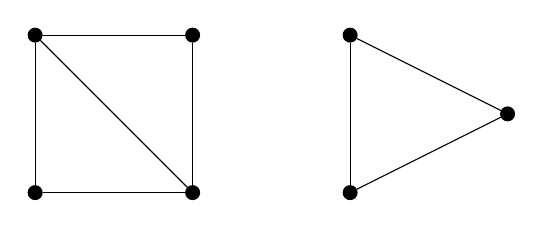
\begin{tikzpicture}[
    vertex/.style={circle, draw, fill=black, minimum size=5pt, inner sep=0pt},
    label distance=2mm  % 调整标签距离线的距离
]

  % 定义顶点位置
  \node[vertex] (x1) at (0,1) {};
  \node[vertex] (x2) at (0,-1) {};
  \node[vertex] (x3) at (2,1) {};
  \node[vertex] (x4) at (2,-1) {};
  \node[vertex] (x5) at (4, 1) {};
  \node[vertex] (x6) at (4, -1) {};
  \node[vertex] (x7) at (6, 0) {};
%  \node[vertex] (x8) at (8, 1) {};
  

  % 绘制有向边并添加数字标签
  \draw[-] (x1) -- (x2);
  \draw[-] (x2) -- (x4);
  \draw[-] (x3) -- (x4);
  \draw[-] (x4) -- (x1);
  \draw[-] (x1) -- (x3);

  \draw[-] (x5) -- (x6);
  \draw[-] (x6) -- (x7);
  \draw[-] (x7) -- (x5);
  
\end{tikzpicture}

A graph $T$ is a tree if $T$is connected; and does not contain q cycle as q subgraph. A graph $F$ is a forest if all components of $F$ are trees. A leaf of a graph is a vertex with degree $1$. Trees, with leaves circled.

\tikzset{every picture/.style={line width=0.75pt}} %set default line width to 0.75pt        

\begin{tikzpicture}[x=0.75pt,y=0.75pt,yscale=-1,xscale=1]
%uncomment if require: \path (0,300); %set diagram left start at 0, and has height of 300

%Straight Lines [id:da8778746157310466] 
\draw    (26.52,180.52) -- (53.81,102.84) -- (99.99,170.51) -- (153.11,106.6) -- (191.04,178.21) -- (236.56,112.35) ;
%Straight Lines [id:da982602405019146] 
\draw    (311.33,94.55) -- (315.4,146.07) -- (361.03,109.46) ;
%Straight Lines [id:da10558162526255566] 
\draw    (315.4,146.07) -- (340.36,179.43) ;
%Straight Lines [id:da9652131386469209] 
\draw    (281.55,176.92) -- (315.4,146.07) ;
%Straight Lines [id:da9098976808427328] 
\draw    (277.55,129.99) -- (315.4,146.07) ;
%Straight Lines [id:da6871756317261613] 
\draw    (458.32,75.75) -- (477.12,97.08) -- (501.63,75.98) ;
%Straight Lines [id:da8528625774476026] 
\draw    (471.01,123.31) -- (477.12,97.08) ;
%Straight Lines [id:da38370950515203894] 
\draw    (505.75,119.91) -- (471.01,123.31) ;
%Straight Lines [id:da11776512824599861] 
\draw    (442.15,144.6) -- (471.01,123.31) ;
%Straight Lines [id:da3101455899284844] 
\draw    (415.7,124.08) -- (442.15,144.6) ;
%Straight Lines [id:da7053915994545827] 
\draw    (507.92,168.38) -- (475.72,173.41) -- (442.15,144.6) ;
%Straight Lines [id:da6541004127841545] 
\draw    (487.63,201.13) -- (475.72,173.41) ;
%Straight Lines [id:da08969264363324325] 
\draw    (428.07,175.9) -- (442.15,144.6) ;
\end{tikzpicture}

\subsection{Problem 3.9 (Minimum Spanning Tree Problem)}
Let $(G, W)$ be a network graph, where $G$ is connected and $w:\ E(G)\to\mathbb{R}$. Find a \uline{minimum spanning tree (MST)}, that is, a spanning tree (ST) $T$ of $G$ s.t. $\sum\limits_{e\in E(T)} w(e)$ is minimum.

\uline{Kruskal's Algorithm} can solve Problem 3.9, and is as follows.

\paragraph{Kruskal's Algorithm}
\begin{itemize}
    \item Choose an edge $e_1\in E(G)$ with $w(e_i)$ minimum.
    \item Suppose edges $e_1,\cdots, e_k\in E(G)$ have been chosen, for some $k\geqslant 1$. Choose $e_{k+1}\in E(G)\backslash\{e_1,\cdots, e_k\}$ s.t. $e_{k+1}$ does not from a cycle with some of $e_1,\cdots, e_k$ and $w(e_{k+1})$ is minimum.
    \item Continue until $|V(G)| - 1$ edges are found. The result is a MST.
\end{itemize}

\setcounter{example}{3}
\begin{example}
    Let $(G, W)$ be

    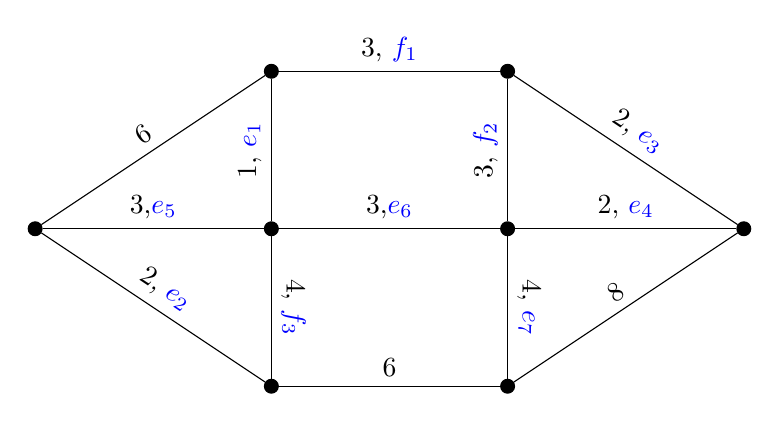
\begin{tikzpicture}[
    vertex/.style={circle, draw, fill=black, minimum size=5pt, inner sep=0pt},
    label distance=1mm  % 调整标签距离线的距离
]

  % 定义顶点位置
  \node[vertex] (x1) at (0,0) {};
  \node[vertex] (x2) at (3,2) {};
  \node[vertex] (x3) at (3,-2) {};
  \node[vertex] (x) at (3,0) {};
  \node[vertex] (y) at (6,0) {};
  \node[vertex] (x4) at (6, 2) {};
  \node[vertex] (x5) at (6, -2) {};
  \node[vertex] (x6) at (9, 0) {};

  % 绘制有向边并添加数字标签
  \draw[-] (x1) -- (x2) node[midway, above, sloped] {6};
  \draw[-] (x1) -- (x3) node[midway, above, sloped] {2, \textcolor{blue}{$e_2$}};
  \draw[-] (x1) -- (x) node[midway, above, sloped] {3,\textcolor{blue}{$e_5$}};
  \draw[-] (x) -- (y) node[midway, above, sloped] {3,\textcolor{blue}{$e_6$}};
  \draw[-] (x) -- (x2) node[midway, above, sloped] {1, \textcolor{blue}{$e_1$}};
  \draw[-] (x) -- (x3) node[midway, above, sloped] {4, \textcolor{blue}{$f_3$}};
  \draw[-] (x2) -- (x4) node[midway, above, sloped] {3, \textcolor{blue}{$f_1$}};
  \draw[-] (x4) -- (x6) node[midway, above, sloped] {2, \textcolor{blue}{$e_3$}};
  \draw[-] (y) -- (x6) node[midway, above, sloped] {2, \textcolor{blue}{$e_4$}};
  
  \draw[-] (y) -- (x4) node[midway, above, sloped] {3, \textcolor{blue}{$f_2$}};
  \draw[-] (x5) -- (x6) node[midway, above, sloped] {8};
  \draw[-] (x3) -- (x5) node[midway, above, sloped] {6};

  \draw[-] (y) -- (x5) node[midway, above, sloped] {4, \textcolor{blue}{$e_7$}};
\end{tikzpicture}
\end{example}

We ``greedily'' choose $e_1,\cdots, e_6$, since they have the smallest weights, and do not from a cycle. Then we cannot choose $f_1$ or $f_2$ since adding either edge forms a cycle. We can then choose $e_7$ (but not $f_3$) to obtain the MST. The weight is $1+2+2+2+3+3+4 = 17$.
    
\begin{tikzpicture}[
    vertex/.style={circle, draw, fill=black, minimum size=5pt, inner sep=0pt},
    label distance=1mm  % 调整标签距离线的距离
]

  % 定义顶点位置
  \node[vertex] (x1) at (0,0) {};
  \node[vertex] (x2) at (3,2) {};
  \node[vertex] (x3) at (3,-2) {};
  \node[vertex] (x) at (3,0) {};
  \node[vertex] (y) at (6,0) {};
  \node[vertex] (x4) at (6, 2) {};
  \node[vertex] (x5) at (6, -2) {};
  \node[vertex] (x6) at (9, 0) {};

  % 绘制有向边并添加数字标签
  \draw[-] (x1) -- (x3) node[midway, above, sloped] {2, \textcolor{blue}{$e_2$}};
  \draw[-] (x1) -- (x) node[midway, above, sloped] {3,\textcolor{blue}{$e_5$}};
  \draw[-] (x) -- (y) node[midway, above, sloped] {3,\textcolor{blue}{$e_6$}};
  \draw[-] (x) -- (x2) node[midway, above, sloped] {1, \textcolor{blue}{$e_1$}};
  \draw[-] (x4) -- (x6) node[midway, above, sloped] {2, \textcolor{blue}{$e_3$}};
  \draw[-] (y) -- (x6) node[midway, above, sloped] {2, \textcolor{blue}{$e_4$}};
  \draw[-] (y) -- (x5) node[midway, above, sloped] {4, \textcolor{blue}{$e_7$}};
\end{tikzpicture}

\begin{theorem}
    Kruskal's Algorithm solves Problem 3.9.
\end{theorem}
\begin{proof}
    Let $|V(G)| = n$. We first show that when the algorithm terminates, we have a $ST$ $T$ of $G$. 

    Initially, we have a forest with $n$ single vertices as components. Suppose that after $t$ iterations $(0\leqslant t\leqslant n-2)$, the current graph $F$ is a forest with $n-t$ components. If we add a new edge $xy$ to $F$ to form $F^+$, then we cannot have $x, y$ belonging to the same component of $F$, otherwise we create a cycle. Also, since $G$ is connected, we may add $xy$ where $x, y$ belong to two different components $F_1, F_2$ of $F$. The new component $F^{\prime} = \left(V(F_1)\cup V(F_2),\ E(F_1)\cup E(F_2) \cup\{xy\} \right)$ of $F^+$ is also a tree. Clearly $F^{\prime}$ is connected, and if $\exists$ cycle $C\subset F^{\prime}$, then $\exists\ e, e^{\prime}\in E(C)$, each one connecting $F_1$ and $F_2$, a contradiction since $xy$ is the only such edge in $F^{\prime}$. Thus, $F^+$ is a forest with $n-t-1$ components. Iterating $n-1$ times gives a ST T of G.

    Now, we prove that $T$ is a MST. Let $e_1,\cdots, e_{n-1}$ chosen in that order, so $w(e_1)\leqslant\cdots\leqslant w(e_{n-1})$. If $T$ is not a MST, choose a MST $S\subset G$ s.t. $|E(S)\cap E(T)|$ is maximum. Let $1\leqslant k \leqslant n-1$ be s.t. $e_1,\cdots, e_{k-1}\in E(S)\cap E(T)$, and $e_k\in E(T)\backslash E(S)$. Then $S^{\prime} = (V(S), E(S)\cup\{e_k\})$ has a cycle $C^{\prime}$. Now, $\exists\ f\in E(C^{\prime})\backslash E(T)$. Then $S^{\prime\prime} = (V(S^{\prime},\ E(S^{\prime})\backslash\{f\})$ is also a ST, since $S^{\prime\prime}$ is connected and has $n-1$ edges (HW6). To see that $S^{\prime\prime}$ is connected, let $u,\ v\in V(S^{\prime\prime}$. Then $\exists\ u-v$ path $P\subset S^{\prime}$. Either $P\subset S^{\prime\prime}$, or $f\in E(P)$. If the latter, let $f= zz^{\prime}$. Then $\exists\ u-z$ and $z^{\prime}-v$ paths $\subset P$, and a $z-z^{\prime}$ path in $C^{\prime}$, not using $f$. These paths $\Longrightarrow$ $\exists\ u-v$ path in $S^{\prime\prime}$. 

    Now $\sum\limits_{e\in E(S^{\prime\prime})} w(e) \geqslant \sum\limits_{e\in E(S)} w(e)\ \Longrightarrow\ w(e_k)\geqslant w(f)$. Since $e_1,\cdots, e_{k-1}, e_k\in E(T)$ and $e_1,\cdots, e_{k-1},f\in E(S)$, neither of these sets of edges creates a cycle, and since the algorithm chose $e_k$ instead of $f$, we have $w(e_k)\geqslant w(f)$. So $w(e_k)=w(f)$, and $S^{\prime\prime}$ is also a MST. But then $|E(S^{\prime\prime})\cap E(T)| = |E(S)\cap E(T)| + 1$, which contradicts the choice of $S$.
\end{proof}

\begin{remark}
    \begin{itemize}
        \item Kruskal's Algorithm also work if some edges of $G$ has negative weights.
        \item If these is a tie for the choice of edges with minimum weight at an iteration, we may choose any suitable edge.
        \item If $G$ has $q$ components, then Kruskal's Algorithm finds a minimum spanning forest in $n-q$ iterations.
    \end{itemize}
\end{remark}

\setcounter{proposition}{10}
\begin{proposition}
    Let $T$ be a tree with $n\geqslant 2$ vertices. 
    \begin{itemize}
        \item[(a)] $T$ has a leaf.
        \item[(b)] Deleting a leaf $x$ and the edge $e$ incident to $x$ from $T$ gives another tree $T^{\prime}$.
    \end{itemize}
\end{proposition}
\begin{proof}
    True for $n=2$. Assume $n\geqslant 3$.
    \begin{itemize}
        \item[(a)] Let $P = x_0 x_1\cdots x_k\subset T$ be a longest path, for some $k\geqslant 2$. Then $\Gamma(x_k)\subset\{x_0,\cdots,x_{k-1}\}$, otherwise we have a path longer than $P$. Also, $x_kx_i\notin E(T)$, $\forall 0\leqslant i\leqslant k-2$, otherwise $T$ has a cycle. So $\Gamma(x_k) = x_{k-1}$, and $x_k$ is a leaf.
        \item[(b)] Clearly $\neq\exists$ cycle in $T\Longrightarrow\ \neq\exists$ cycle in $T^{\prime}$. Let $u,v\in V(T^{\prime}) = V(T)\backslash\{x\}$. Then $\exists u-v$ path $Q\subset T$, and $Q$ cannot use $e$ and $x$ since $d(x)= 1$ in $T$. So $G\subset T^{\prime}$ and $T^{\prime}$ is connected.
    \end{itemize}
\end{proof}

Prop 3.11 is very useful for induction proofs involving trees.




\chapter{Queueing Theory}
\section{Queueing system}
Queueing happens in everyday life. At the supermarket or airport, bank and so on. A typical queueing system (say at the airport check-in): 


Suppose the $n^{th}$ customer $C_n$ arrives at time $\tau_n\geqslant 0$, where $\tau_n =0$ and $0\leqslant \tau_1\leqslant \tau_2\leqslant \cdots\leqslant $. The \uline{interarrival time} between customers $c_n$ and $c_{n+1}$ is $T_n = \tau_{n+1} - \tau_n\ (T_0 = \tau_1)$. The \uline{service time} for customer $C_n$ is $X_n\geqslant 0$. Assume the $T_n$ are independent random variables, and the some for the $X_n$. The \uline{distribution function (DF)} of $T_n(n\geqslant 0)$ is $A_n:\mathbb{R}\to [0, 1]$, where
\begin{align*}
    A_n(t) = \mathbb{P}(T_n\leqslant t)
\end{align*}
and the \uline{probability density function (PDF)} is 
\begin{align*}
    a_n(t) = A_n^{\prime}(t)
\end{align*}

Similarly, $X_n\ (n\geqslant 1)$ has DF $B_n(t) = \mathbb{P}(X_n\leqslant t)$ and PDF $b_n(t) = B_n^{\prime}(t)$. 

\paragraph{Kendall-Lee notation} A queueing system description is written as:

\vspace{1em}
\begin{align}
    \eqnmarkbox[red]{A}{A}/\eqnmarkbox[blue]{B}{B}/\eqnmarkbox[green]{s}{s}/\eqnmarkbox[pink]{D}{D}/\eqnmarkbox[brown]{q}{q}/\eqnmarkbox[orange]{p}{p} \label{4.1}
\end{align}
\annotate[yshift=0.5em]{above,left}{A}{Interarrival time distribution}
\annotate[yshift=2.0em]{above,left}{B}{Service time distribution}
\annotate[yshift=-0.5em]{below, left}{s}{Number of servers}
\annotate[yshift=-0.5em]{below,right}{D}{Queueing discipline}
\annotate[yshift=2.0em]{above,right}{q}{Maximum number of customers allowed in the queueing system\\ (in queue and in service)}
\annotate[yshift=0.5em]{above,right}{p}{Customer population}

\paragraph{Notable cases:}
For $A$ and $B$:
\begin{itemize}
    \item $M$: \uline{Markovian}, with \uline{exponential distribution}
    \begin{align*}
        A_n(t) = 1-e^{-\lambda_n t},\quad a_n(t) = \lambda_n e^{-\lambda_n t}
    \end{align*}
    for some parameter $\lambda_n > 0\ (n\geqslant 0)$. Similarly for $B_n(t)$, $b_n(t)$ with parameter $\mu_n>0\ (n\geqslant 1)$.
    \item $D$: \uline{Deterministic}, with ``constant distribution''.
    \item $E_k$: \uline{Erlang-k}
    \item $G$: \uline{General}, not specified, usually the mean and variance are known.
\end{itemize}

For $D$:
\begin{itemize}
    \item FCFS: \uline{First come first served}. Services is performed according to the order of the queue. New arrival join the back of the queue.
    \item LCFS: \uline{Last come first served}. 
    \item SIRO: \uline{Service in random order}.
\end{itemize}

\paragraph{Note also} Nucleic acid test queueing discipline. 

Arrival order: $1,2,\cdots, 20, 21, 22, \cdots, 40, 41, \cdots$

Service order: $20, 19, \cdots, 40, 39,\cdots, 21, 60, \cdots$

For example, $M/G/2/SIRO/50/1000$. If $D = FCFS$, $q=p=\infty$, then we write \ref{4.1} as $A/B/s$. The simplest case is $M/M/s$, especially $M/M/1$.

\begin{definition}
    
    \begin{itemize}
        \item \uline{State/Queue length}$=$ Number of customers in the queueing system/queue (12 and 8 in the diagram).
        \item $N(t) = $ State at time $t\geqslant 0$.
        \item $\mathbb{P}_k(t) = $ Probability of state $k$ at time $t\geqslant 0$ (assume $\mathbb{P}_k(0) = 0$).
        \item $\lambda_k = $ Mean arrival rate $=$ Expected number of new customer arrivals per unit time, when state $=k\geqslant 0$.
        \item $\mu_k = $ \uline{Mean service rate for overall system} $=$ Expected number of customers served per unit time between all \uline{busy} servers (those serving customers), when state $= k\geqslant 1$.
    \end{itemize}
\end{definition}

When $A$ and $B$ are both Markovian, we have the \uline{birth-death process rate diagram}:
\usetikzlibrary{automata}
\begin{tikzpicture}[->, >=stealth', auto, thick, node distance=2cm]

\tikzstyle{every state}=[fill=white, draw=black, text=black, minimum size=1.2cm]

\node[state] (q0) {$0$};
\node[state] (q1) [right of=q0] {$1$};
\node[state] (q2) [right of=q1] {$2$};
\node[state] (q3) [right of=q2] {$3$};

\path[->, draw=blue] 
    (q0) edge[bend left] node[above] {$\lambda_0$} (q1)
    (q1) edge[bend left] node[above] {$\lambda_1$} (q2)
    (q2) edge[bend left] node[above] {$\lambda_2$} (q3)
    (q3) edge[bend left] node[above] {$\lambda_3$} ($(q3)+(1,0)$);

\path[->, draw=red]
    (q1) edge[bend left] node[below] {$\mu_1$} (q0)
    (q2) edge[bend left] node[below] {$\mu_2$} (q1)
    (q3) edge[bend left] node[below] {$\mu_3$} (q2)
    ($(q3)+(1,0)$) edge[bend left] node[below] {$\mu_4$} (q3);

\end{tikzpicture}

If $\lambda_k$ is constant $\forall k\geqslant 0$, write $\lambda_k = \lambda$. If the mean service rate \uline{per busy server} is constant $\forall k\geqslant 1$, denote this constant by $\mu$. Then 
\begin{align*}
    \mu_k = \left\lbrace\begin{array}{ll}
       k_{\mu} & 1\leqslant k\leqslant s \\
        s\mu & k>s.
    \end{array} \right.
\end{align*}

Under these circumstance, $\frac{1}{\lambda}$ and $\frac{1}{\mu}$ are the \uline{expected interarrival time} and the \uline{expected service time}.

Also,
\begin{align*}
    \varrho = \frac{\lambda}{s\mu}
\end{align*}

is the \uline{utilisation factor} of the service facility, which is the expected fraction of time the service capacity $(s\mu)$ is being utilised by arriving customers $(\lambda)$.

\begin{example}
    Suppose a time unit is one hour.
    \begin{itemize}
        \item If on average, a customer arrives every 10 minutes, then $\lambda = 6$ customers/hour. Expected interarrival time $\frac{1}{\lambda} = \frac{1}{6}$.
    
        \item If on average, a service time takes 30 minutes, then $\mu = 2$ customers/hour. Expected service time $= \frac{1}{\mu} = \frac{1}{2}$.
    \end{itemize}
    Utilisation factor $\varrho = \frac{\lambda}{s\mu} = \frac{3}{s}$.
    \begin{itemize}
        \item If $s = 1,2$, then $\varrho>1$. The state $\to\infty$ as time $\to\infty$, and the system is ``unsteady''.
        \item If $s = 3$, then $\rho = 1$. Queue is unstable and system may not become ``steady''.
        \item If $s\geqslant 4$, then $\rho <1$. The system will become ``steady''. 
    \end{itemize}
\end{example}

\begin{definition}
    \begin{align}
        \eqnmarkbox[blue]{1}{\bar{L}(t)} &= \frac{1}{t}\int_0^t N(u)du \nonumber \\
        \eqnmarkbox[red]{2}{\bar{L}} &= \lim\limits_{t\to\infty} \bar{L}(t) \nonumber \\
        & {} \nonumber \\
        \eqnmarkbox[orange]{4}{\bar{\alpha}(t)} &= \frac{\eqnmarkbox[green]{3}{\alpha(t)}}{t} \nonumber \\
        \eqnmarkbox[pink]{5}{\bar{\lambda}} &= \lim\limits_{t\to\infty} \bar{\alpha(t)}  \label{4.2}
    \end{align}
    \annotate[yshift=0.5em]{above,right}{1}{The average state over $[0,t]$}
    \annotate[yshift = 0.5em]{above,left}{2}{The long term average state}
    \annotate[yshift = 0.5em]{above,right}{3}{Number of arrivals in $[0,t]$}
    \annotate[yshift = 0.5em]{above,left}{4}{The average number of arrivals in $[0,t]$}
    \annotate[yshift = -0.5em]{below,left}{5}{The long term average arrival rate}

    \begin{itemize}
        \item \uline{Sojourn time} $=$ Time a customer spends in queueing system.
        \item $W_k = $ Sojourn time of customer $C_k$.
        \item $\bar{W}(t) = \frac{1}{\alpha(t)}\sum\limits_{k=1}^{\alpha(t)} W_k$, the \uline{average sojourn time} in $[0,t]$.
        \begin{align}
            \bar{W} = \lim\limits_{t\to\infty} \frac{1}{n} \sum\limits_{k=1}^n W_k \label{4.3}
        \end{align}
        the \uline{long term average sojourn time}
    \end{itemize}
\end{definition}

\begin{theorem}[Little' Low]
    For any queueing system, 
    \begin{align}
        \overline{L} = \overline{\lambda}                                    \ \overline{W}, \label{4.4}
    \end{align}
    provided the limits \ref{4.2}, \ref{4.3} exist.
\end{theorem}
\begin{proof}
    Let $\beta(t)$ be the number of departures in $[0,t]$. We compare the graphs of $\alpha(t)$, $\beta(t)$, and the sojourn times.


    Let $E(t)$ be the excess sojourn time of all active customers beyond time $t$. Then 
    \begin{align*}
        \overline{L}(t) &= \frac{1}{t}\int_0^t N(u)du = \frac{1}{t}\int_0^t (\alpha(u) - \beta(u)) du \\
        &= \frac{\alpha}{t} \frac{1}{\alpha} \left(\sum\limits_{k=1}^{\alpha(t)}W_k - E(t) \right) = \bar{\alpha}(t) \overline{W(t)} - \frac{E(t)}{t}
    \end{align*}

    Letting $t\to\infty$ and assuming $\frac{E(t)}{t}\to 0$, \ref{4.4} follows.
\end{proof}

\begin{remark}
    If $\overline{L}(q) = $ Long term average queue length, $\overline{W}_q = $ Long term average queueing time, then we can similarly prove that
    \begin{align*}
        \overline{L}_q = \overline{\lambda}\ \overline{W}_q
    \end{align*}
    Also, if the expected service time $\frac{1}{\mu}$ is constant, then
    \begin{align*}
        \overline{W} = \overline{W}_q + \frac{1}{\mu}
    \end{align*}
\end{remark}

\begin{example}
    Bob owns a small coffee shop. He estimates that on average, in one hour, 40 customers arrive at his shop, and each customer spends 6 minutes in the queueing system. Then the average number of customers in the queueing system is 
    \begin{align*}
        \overline{L} = \eqnmarkbox[red]{1}{40}\times \eqnmarkbox[orange]{2}{0.1} = 4
    \end{align*}
    \annotate[yshift=-0.5em]{below,left}{1}{$\overline{\lambda}$}   
    \annotate[yshift=-0.5em]{below,right}{2}{$\overline{W}$}    
\end{example}

\begin{figure}[H]
    \centering
    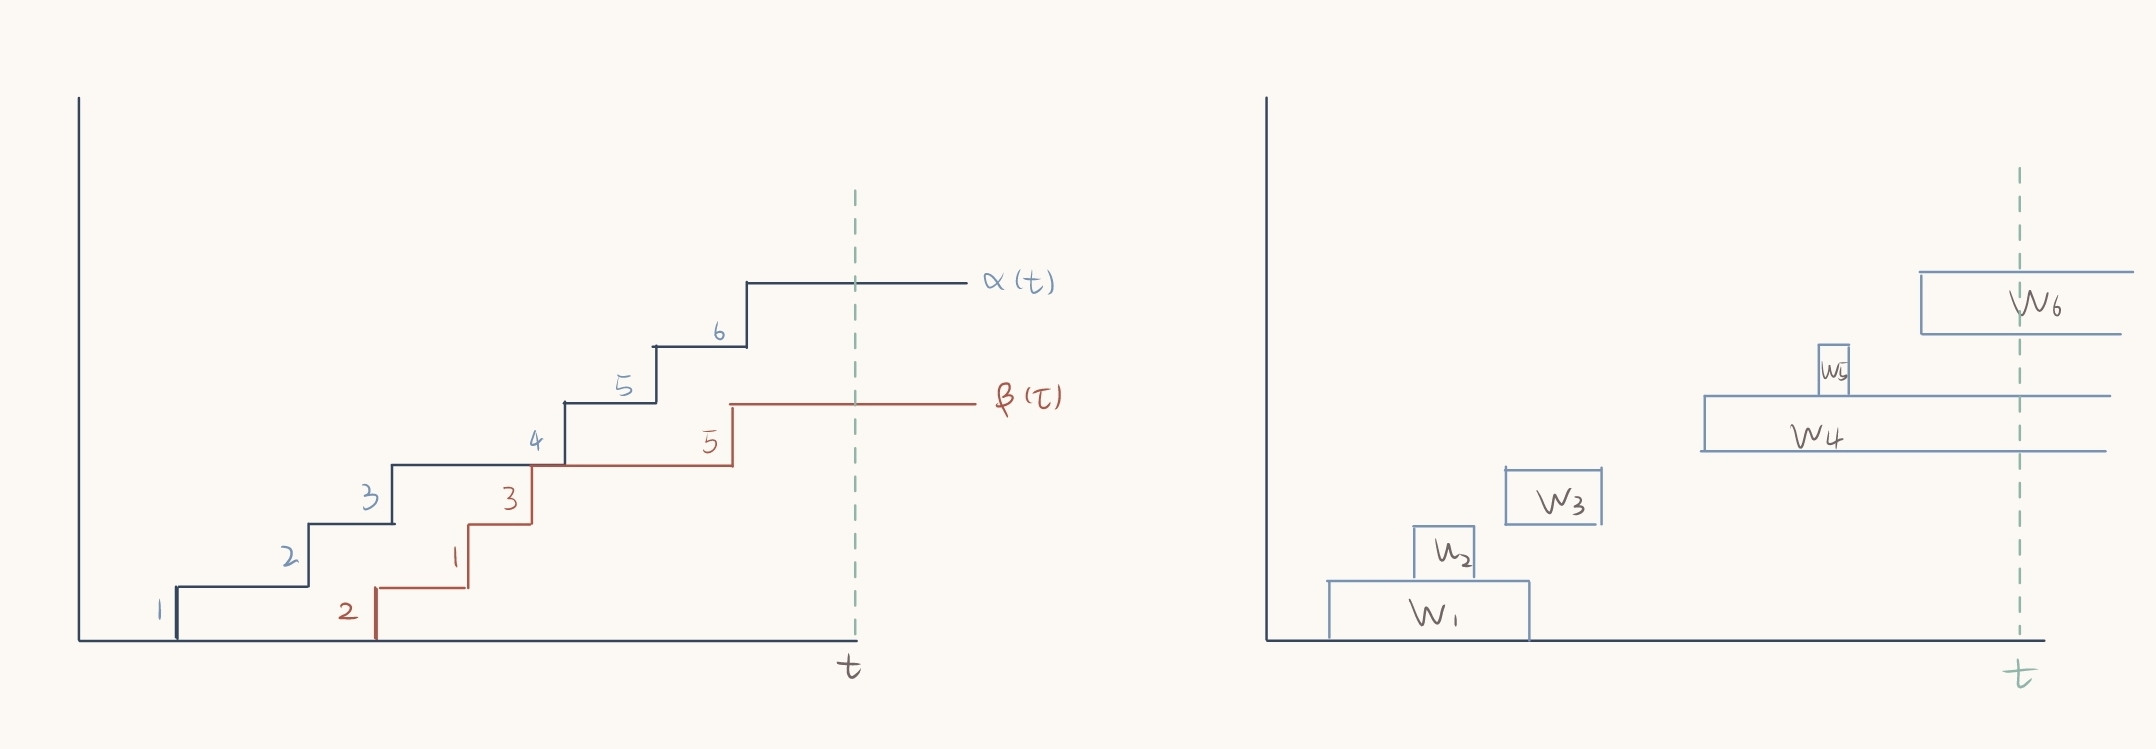
\includegraphics[width=\textwidth]{document/4-1.jpg}
\end{figure}

\section{The exponential distribution}
Recall that in a Markovian queueing system. $A/B/s$ both $A=M$(interarrival time) and $B = M$(service time) follow the exponential distributions, with DF and PDF of the form

\begin{align*}
    F(t) &= \mathbb{P}(T\leqslant t) = \left\lbrace\begin{array}{ll}
        1 - e^{-\gamma t} &\ \text{if}\ t\geqslant 0 \\
        0 & \ \text{if} \ t<0
    \end{array} \right. \\
    f(t) & = \left\lbrace\begin{array}{ll}
        \gamma e^{-\gamma t} &\ \text{if}\ t\geqslant 0 \\
        0 & \ \text{if} \ t<0
    \end{array} \right.
\end{align*}
for some $\gamma>0$, where $T$ is the $A$ or $B$ RV. We have 
\begin{align*}
    \mathbb{E} T &= \int_0^{\infty} \gamma u e^{-\gamma u} du = \frac{1}{\gamma} \\
    \text{var} T &= \mathbb{E}(T^2) - (\mathbb{E} T)^2 = \int_0^{\infty} \gamma u^2 e^{-\gamma u} du - \frac{1}{\gamma^2} = \frac{1}{\gamma^2}
\end{align*}

\setcounter{proposition}{1}
\begin{proposition}
    $f(t)$ is strictly decreasing for $t\geqslant 0$. Thus, 
    \begin{align*}
        \mathbb{P}(0\leqslant T\leqslant h) > \mathbb{P}(t\leqslant T\leqslant t+h),\quad \forall t,h >0
    \end{align*}
    \begin{figure}[H]
        \centering
        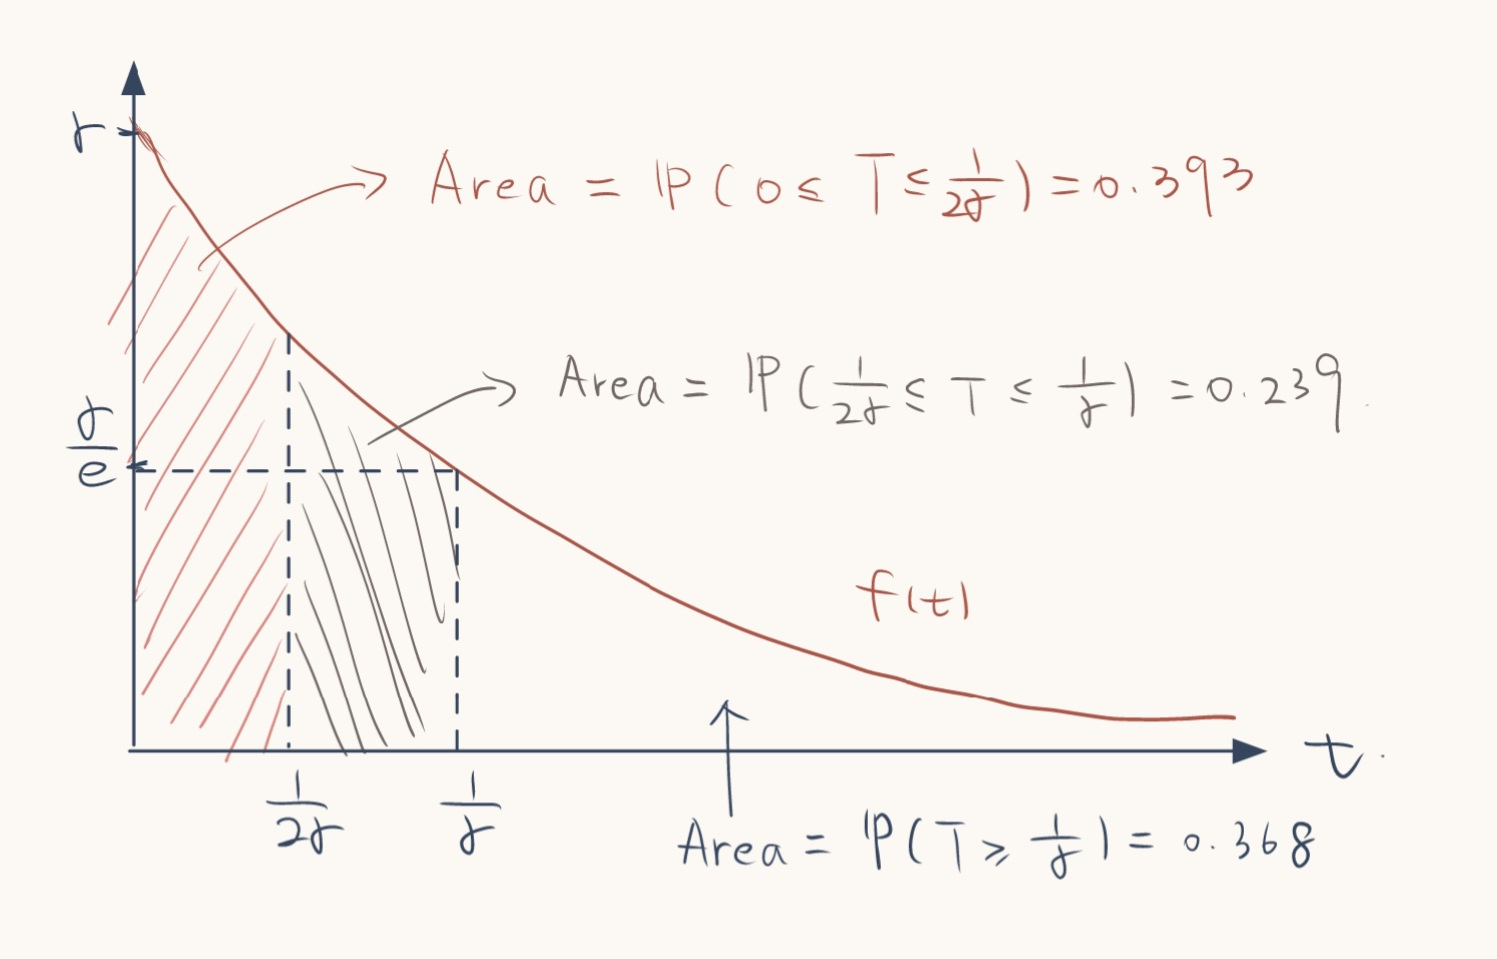
\includegraphics[width = 0.6\textwidth]{document/4-2.jpg}
    \end{figure}
\end{proposition}

\paragraph{Recall} For events $E_1,E_2$ in a probability space, the \uline{conditional probability} of $E_1$, gives $E_2$, is
\begin{align*}
    \mathbb{P}(E_1\mid E_2) = \frac{\mathbb{P}(E_1\cap E_2)}{\mathbb{P}(E_2)}
\end{align*}

\begin{proposition}[Lack of memory]
    \begin{align*}
        \mathbb{P}(T>t+h\mid T>h) = \mathbb{P}(T>t) \quad \forall t,h>0
    \end{align*}
    That is, the probability distribution of the remaining time until the event (arrival or service completion) occurs is always the same, regardless of how much time $h$ has already passed. There is no memory of what has already occurred.
\end{proposition}
\begin{proof}
    \begin{align*}
        \mathbb{P}(T>t+h\mid T>h) &= \frac{\mathbb{P}(T>t+h\ \text{and}\ T>h)}{\mathbb{P}(T>h)} = \frac{\mathbb{P}(T>t+h)}{\mathbb{P}(T>h)} \\
        &= \frac{e^{-\gamma (t+h)}}{e^{-\gamma h}} = e^{-\gamma t} = \mathbb{P}(T>t)
    \end{align*}
\end{proof}

\begin{proposition}
    Let $T_1,\cdots,T_n$ be independent exponential RVs with parameters $\gamma_1,\cdots,\gamma_n$. Then the RV 
    \begin{align*}
        U = \min(T_1,\cdots, T_n)
    \end{align*}
    has an exponential distribution with parameter $\gamma = \gamma_1 + \cdots + \gamma_n$. Thus, if $T_i$ represents the time until the $i^{\text{th}}$ event occurs, then $U$ represents the time until the first of the $n$ events occurring. 
\end{proposition}
\begin{proof}
    \begin{align*}
        \mathbb{P}(U>t) &= \mathbb{P}(T_1>t,\cdots, T_n>t\ \text{all hold}) \\
        & = \eqnmarkbox[blue]{1}{\mathbb{P}(T_1>t) \cdots \mathbb{P}(T_n>t)} \\
        & = e^{-\gamma_1 t} \cdots e^{-\gamma_n t} = e^{-\gamma t}
    \end{align*}
    \annotate[yshift=2.5em]{above,right}{1}{By independence}
    
\end{proof}

In particular, if $X_1,\cdots,X)s$ are the independence service times, each exponential with parameter $\mu$, then $U$ is the time until the next service completion, which is the exponential with parameter $s\mu$.

\subsubsection{Relationship with Poisson distribution and process}
Suppose the time between consecutive occurrences of some kind of event (For example, interarrivals) has an exponential distribution with parameter $\gamma$. Let $Y(t)$ be the number of event occurrences at time $t\geqslant 0$. Then $Y(t)$ is a RV with the Poisson Distribution with parameters $\gamma t$, given by
\begin{align*}
    \mathbb{P}(Y(t) = k) = \frac{(\gamma t)^k e^{-\gamma t}}{k!},\quad  \text{for}\ k=0,1,2,\cdots
\end{align*}
When the events are counted on a continuing basis, the counting process $\{Y(t):t\geqslant 0\}$ is a \uline{Poisson process} with mean rate $\gamma$.

\begin{proposition}
    \begin{align*}
        \mathbb{P}(T\leqslant t+h\mid T>t) \approx \gamma h,\quad \forall t>0\ \text{and small}\ h
    \end{align*}
\end{proposition}
\begin{proof}
    \begin{align*}
        \mathbb{P}(T\leqslant t+h\mid T>t) &= \frac{\mathbb{P}(T\leqslant t+h\ \text{and}\ T>t)}{\mathbb{P}(T>t)} \\
        &= \frac{(1-e^{-\gamma(t+h)}) - (1-e^{-\gamma t})}{e^{-\gamma t}} \\
        &= 1 - e^{-\gamma h} \approx \gamma h \ \text{for small}\ h
    \end{align*}
\end{proof}

Note that Prop 4.3 says that the probability of an event occurring within an interval of fixed length $h$ is constant, regardless of how much time has passed. Prop 4.5 says that if $h$ is small, then this constant probability is approximately $\gamma h$.


\section{Birth-Death Process and M/M/s Systems}
Recall that $\mathbb{P}_k(t) = $ Probability that state $=k\geqslant 0$ at time $t\geqslant 0$ in a queueing system.
\begin{definition}
    A queueing system is in \uline{transient state} if $\mathbb{P}_k(t)$ depends on $t$. The system becomes \uline{steady state} if $\mathbb{P}_k(t)$ becomes independent of $t$ if $t\geqslant t_1$ for some (large) time $t_1$. If the system is in steady state, let
    \begin{align*}
        p_k = \text{Probability that state} = k \geqslant 0
    \end{align*}
    The \uline{birth-death process} describe the state of a queueing system over time. If the system is Markovian, we assume the following:
    \begin{itemize}
        \item[(1)] Given $N(t) = k$, the probability distributions of the remaining times until the next ``birth'' (arrival) and next ``death'' (departure) are exponential with parameters $\lambda_k,\mu_k$.
        \item[(2)] All RVs in (1) are mutually independent. The next change in state is 
        
        \begin{center}
            \begin{tabular}{lll}
            either: & $k\to k+1$ & (a birth) \\
            or: & $k\to k-1$ & (a death)
        \end{tabular}
        \end{center}     
    \end{itemize}
\end{definition}

\begin{remark}
    By Prop 4.3, for the Markovian birth-death process, the future depends only on the current state, and is independent of any past events. The process is thus a \text{continuous time Markov chain}.
\end{remark}

The relation of the exponential distribution to the Poisson process implies that the $\lambda_k$ and $\mu_k$ are mean rates.

Assume that a queueing system can reach steady state. Let $u_k(t)$ and $v_k(t)$ be the number of times the birth-death process enters and leave state $k$ in $[0,t]$. Then $|u_k(t) - v_k(t)| \leqslant 1$, so
\begin{align*}
    \lim\limits_{t\to\infty} \left|\frac{u_k(t)}{t} - \frac{v_k(t)}{t}\right| = 0
\end{align*}

Since $\frac{u_k(t)}{t}$ and $\frac{v_k(t)}{t}$ are the mean rates at which the process enters and leaves state $k$, we have:
\begin{proposition}[Rate in $=$ Rate out Principle]
    For any state $k\geqslant 0$ in a Markovian birth-death Process, 
    \begin{align}
        \text{Mean entering rate}=\text{Mean leaving rate} \label{4.5}
    \end{align}

    An equation of the form \ref{4.5} is a \uline{balance equation}.
\end{proposition}

For state $0$, the process may only enter from state 1. In steady state, since $p_1$ is the proportion of time that the process can enter state $0$, the mean entering rate to state $0$ is $\mu_1 p_1$. Similarly, the mean leaving rate from state $0$ is $\lambda_0 p_0$. Thus \ref{4.5}$\Rightarrow$
\begin{align}
    \mu_1 p_1 = \lambda_0 p_0 \label{4.6}
\end{align}

For any other state $k\geqslant 1$, we similarly have 
\begin{align}
    \lambda_{k-1}p_{k-1} + \mu_{k+1}p_{k+1} = (\lambda_k + \mu_k) p_k \label{4.7}
\end{align}
Now, \ref{4.6} $\Rightarrow\ \mu_1 p_1 - \lambda_0 p_0 = 0$. And \ref{4.7} $= \mu_{k+1}p_{k+1} - \lambda_k p_k = \mu_k p_k - \lambda_{k-1}p_{k-1}$, $\forall k\geqslant 1$. Thus $\mu_k p_k - \lambda_{k-1}p_{k-1} = 0$, $\forall k\geqslant 0$.

We have
\begin{align*}
    p_k &= \frac{\lambda_{k-1}}{\mu_k} p_{k-1} + \frac{1}{\mu_k} \left(\mu_{k-1}p_{k-1} - \lambda_{k-2}p_{k-2} \right) = \frac{\lambda_{k-1}}{\mu_k} p_{k-1}  \\
    &= \cdots = \frac{\lambda_{k-1}\lambda_{k-2}\cdots \lambda_0}{\mu_k \mu_{k-1}\cdots \mu_0} p_0
\end{align*}

Let
\begin{align}
    r_k = \frac{\lambda_{k-1}\lambda_{k-2}\cdots\lambda_0}{\mu_k\mu_{k-1}\cdots \mu_0},\ \forall k\geqslant 1,\quad \text{and}\ r_0 = 1 \label{4.8}
\end{align}

Then $p_k = r_kp_0$, $\forall k\geqslant 0$. Since $\sum\limits_{k=0}^{\infty} p_k = 1$, we have
\begin{align}
    p_0 = \left( \sum\limits_{k=0}^{\infty} r_k\right)^{-1} \label{4.9}
\end{align}

We remark that steady state cannot be reached if $\lambda_k,\mu_k$ are s.t. $\sum\limits_{k=0}^{\infty} r_k = \infty$. If $\lambda,\mu$ and $\rho = \frac{\lambda}{s\mu}$ are as in section 4.1, then steady state can be reached if $\rho < 1$.

If $s$, $\overline{L}$, $\overline{L}_q$ as defined in section 4.1, and $\overline{\lambda}$ is as in \ref{4.2}, then 
\begin{align}
    \overline{L} = \sum\limits_{k=0}^{\infty} kp_k,\quad \overline{L}_q = \sum\limits_{k=s}^{\infty} (k-s)p_k,\quad \text{and} \quad \overline{\lambda} = \sum\limits_{k=0}^{\infty} \lambda_k p_k \label{4.10}
\end{align}

Now, consider the M/M/1 system. For $\lambda, \mu,\rho$ as above, with $\rho = \frac{\lambda}{\mu} < 1$, we have

\ref{4.8} $\Rightarrow\ r_k = \left(\frac{\lambda}{\mu}\right)^k = \rho^k$, $\forall k\geqslant 0$.

\ref{4.9} $\Rightarrow\ p_o = \left(\sum\limits_{k=0}^{\infty} r_k\right)^{-1} = \left(\sum\limits_{k=0}^{\infty} \rho^k \right)^{-1} = 1 - \rho$.

\ref{4.10} $\Rightarrow\ \overline{L} = \sum\limits_{k=0}^{\infty} kp_k = \sum\limits_{k=0}^{\infty} kr_kp_0 = (1-\rho) \sum\limits_{k=0}^{\infty} k\rho^k = (1-\rho) \rho \frac{d}{d\rho}\sum\limits_{k=0}^{\infty} \rho^k = (1-\rho) \rho \frac{d}{d\rho} \frac{1}{1-\rho} = \frac{\rho}{1-\rho} = \frac{\lambda}{\mu - \lambda}$

Similarly, \ref{4.10} $\Rightarrow$
\begin{align*}
    \overline{L}_q &= \sum\limits_{k=1}^{\infty} (k-1)p_k = \overline{L} - (1-p_0) = \frac{\lambda^2}{\mu(\mu - \lambda)}
\end{align*}

Note that if $\rho = \frac{\lambda}{\mu} > 1$, then $\sum\limits_{k=0}^{\infty} r_k = \sum\limits_{k=0}^{\infty} \rho^k = \infty$, and we cannot have steady state.

Back to $\rho<1$. Let $W$ be a sojourn time RV. If the customer $C$ finds $k$ customers in the queue, then $C$ has to wait through $k + 1$ service times, including $C$'s own, but not the customer currently in service (see Prop 4.3). If $X_1,\cdots, X_{k+1}$ are the RVs of the service times, each exponential with parameter $\mu$, then letting $S_{k+1} = X_1 + \cdots + X_{k+1}$, $k\geqslant 0$, we have
\begin{align*}
    \mathbb{P}(W>t) = \sum\limits_{k=0}^{\infty} p_k \mathbb{P}(S_{k+1}>t)
\end{align*}

It can be shown from this that 
\begin{align*}
    \mathbb{P}(W>t) = e^{-\mu(1-\rho)t},\quad t\geqslant 0
\end{align*}

Thus, $W$ has the exponential distribution with parameter $\mu(1\rho)$, and 
\begin{align*}
    \mathbb{E} W = \frac{1}{\mu(1-\rho)} = \frac{1}{\mu - \lambda}
\end{align*}

Similarly, let $W_q$ be a queueing time RV. If $C$ finds no customers already in the system, then $\mathbb{P}(W_q = 0) = 1-\rho$. If $c$ finds $k\geqslant 1$ customers in the system, then $C$ has to wait through $k$ service times, so 
\begin{align*}
    \mathbb{P}(W_q > t) &= \sum\limits_{k=1}^{\infty} p_k \mathbb{P}(S_k>t) = \sum\limits_{k=1}^{\infty} (1-\rho)\rho^k \mathbb{P}(S_k>t) \\
    &= \rho\sum\limits_{k=0}^{\infty} p_k \mathbb{P}(S_{k+1}>t) = \rho\mathbb{P}(W>t) \\
    & = \rho e^{-\mu(1-\rho)t},\quad t\geqslant 0
\end{align*}

And $\mathbb{E} W_q = \mathbb{E} W - \frac{1}{\mu} = \frac{\lambda}{\mu(\mu - \lambda)}$.





%\newpage 
%1










%\newpage
%\chapter{Appendix}
%\section{Handout 26-3-24}\label{handout 3.26}
%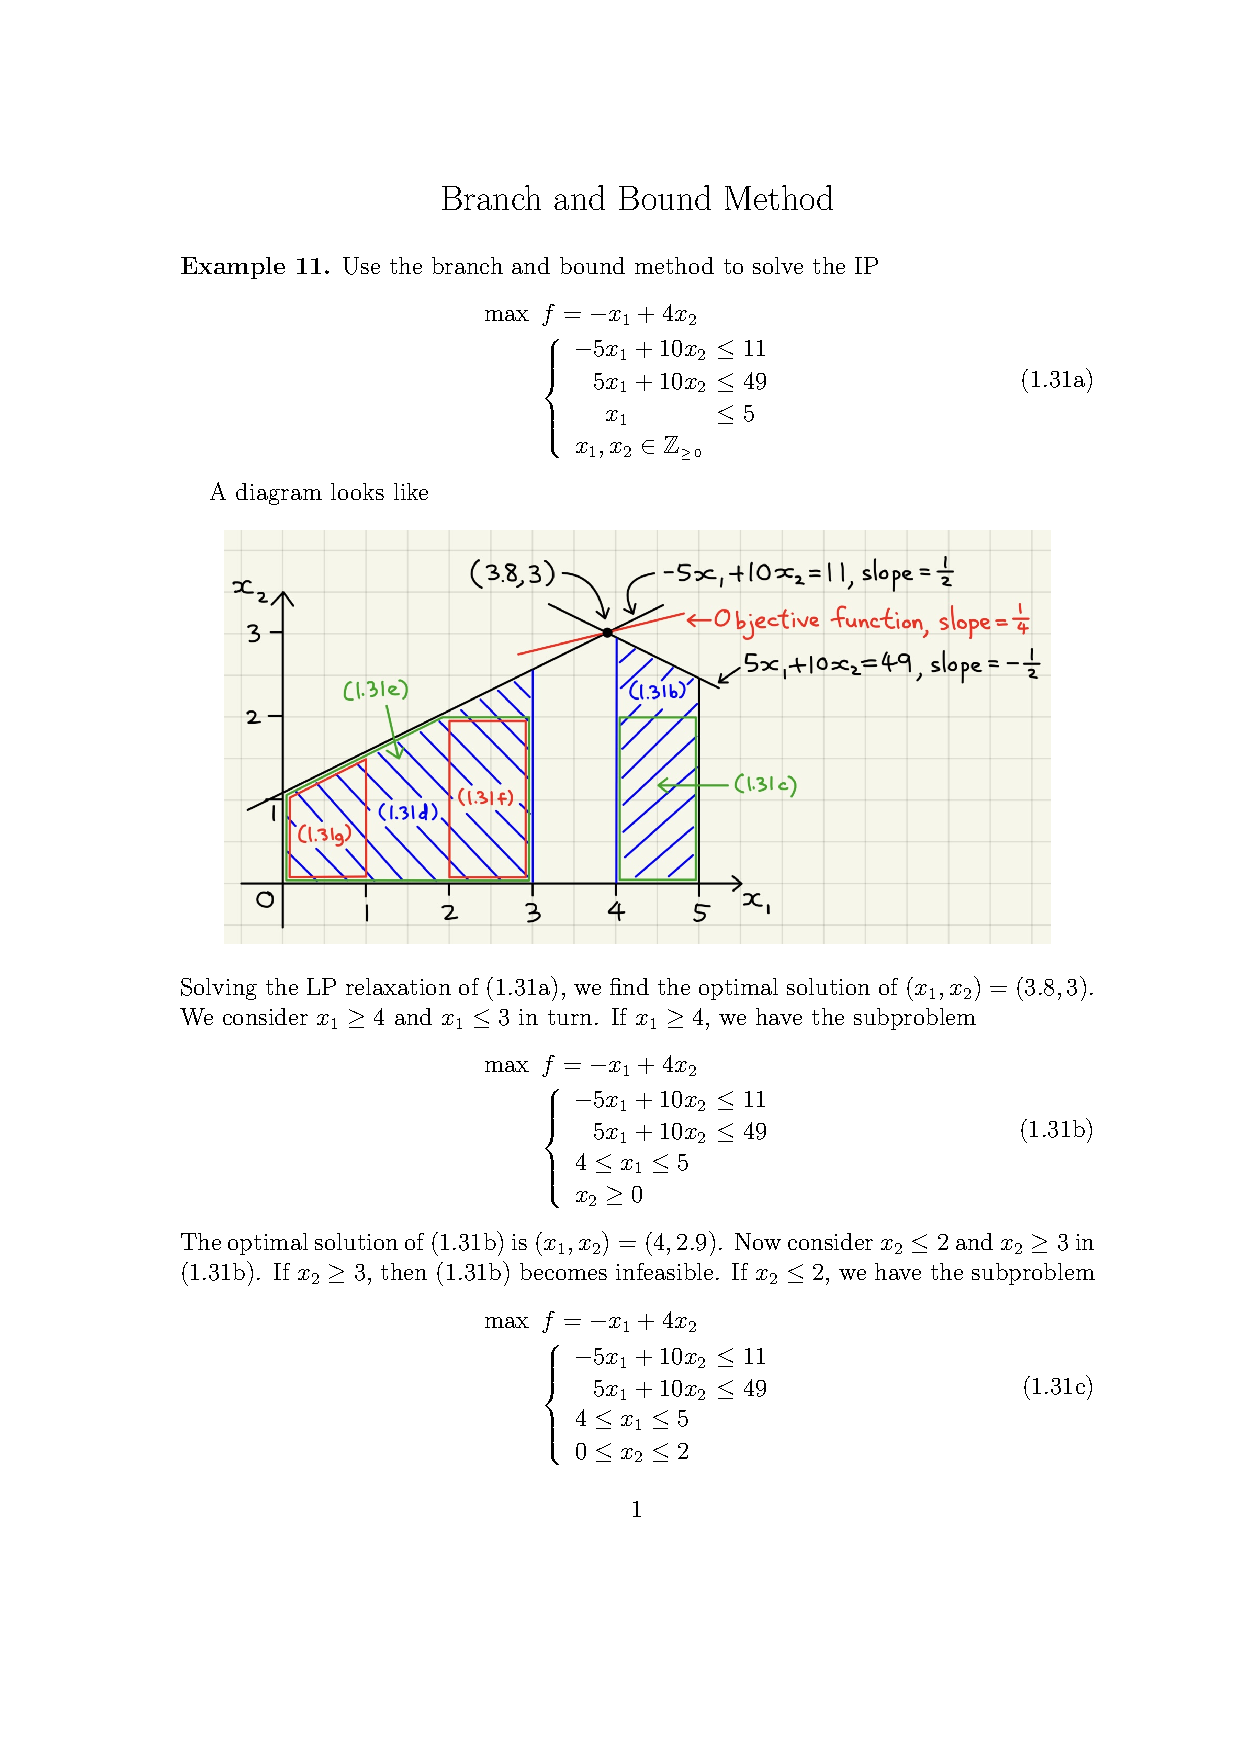
\includepdf[pages = {1-4}, width = 1.3\textwidth]{document/Handout_26-3-24 3.pdf}



\end{document}